
\documentclass[aspectratio=169,xcolor=dvipsnames]{beamer}
%\usetheme{SimplePlus}

\usepackage{hyperref}
\usepackage{graphicx} % Allows including images
\usepackage{booktabs} % Allows the use of \toprule, \midrule and \bottomrule in tables

%----------------------------------------------------------------------------------------
%	TITLE PAGE
%----------------------------------------------------------------------------------------

\title[RegTek]{Grunnleggende reguleringsteknikk} % The short title appears at the bottom of every slide, the full title is only on the title page
%\subtitle{Subtitle}

\author[Fred-Olav] {Fred-Olav Mosdal}

\institute[NTU] % Your institution as it will appear on the bottom of every slide, may be shorthand to save space
{
    Department of Computer Science and Information Engineering \\
    National Taiwan University % Your institution for the title page
}
\date{\today} % Date, can be changed to a custom date


%----------------------------------------------------------------------------------------
%	PRESENTATION SLIDES
%----------------------------------------------------------------------------------------

\begin{document}
\filbreak
\begin{frame}
\frametitle{Grunnleggende prinsipper for tilbakekoblet regulering}
	$$\includegraphics[height=4cm]{cont01.eps}$$
\end{frame}
%Before we begin our discussion on process control, we must define a few key terms.  First, we have what is known as the \textit{process}: the physical system we wish to monitor and control.  For the sake of illustration, consider a heat exchanger that uses high-temperature steam to transfer heat to a lower-temperature liquid.  Heat exchangers are used frequently in the chemical industries to maintain the necessary temperature of a chemical solution, so the desired blending, separation, or reactions can occur.  A very common design of heat exchanger is the ``shell-and-tube'' style, where a metal shell serves as a conduit for the chemical solution to flow through, while a network of smaller tubes runs through the interior of the shell, carrying steam or some other heat-transfer fluid.  The hotter steam flowing through the tubes transfers heat energy to the cooler process fluid surrounding the tubes, inside the shell of the heat exchanger: \index{Process} \index{Heat exchanger}


%In this case, the \textit{process} is the entire heating system, consisting of the fluid we wish to heat, the heat exchanger, and the steam delivering the required heat energy.  In order to maintain steady control of the process fluid's exiting temperature, we must find a way to measure it and represent that measurement in signal form so it may be interpreted by other instruments taking some form of control action.  In instrumentation terms, the measuring device is known as a \textit{transmitter}, because it \textit{transmits} the process measurement in the form of a signal.  

\filbreak

%Transmitters are represented in process diagrams by small circles with identifying letters inside, in this case, ``TT,'' which stands for \textbf{T}emperature \textbf{T}ransmitter:
 
\begin{frame}
\frametitle{Grunnleggende prinsipper for tilbakekoblet regulering}
	$$\includegraphics[height=4cm]{cont02.eps}$$
\end{frame}

%The signal output by the transmitter (represented by the ``PV'' dashed line), representing the heated fluid's exiting temperature, is called the \textit{process variable}.  Like a variable in a mathematical equation that represents some story-problem quantity, this signal represents the measured quantity we wish to control in the process. \index{Process variable}

%In order to exert control over the process variable, we must have some way of altering fluid flow through the heat exchanger, either of the process fluid, the steam, or both.  Generally, it makes more sense to alter the flow of the heating medium (the steam), and let the process fluid flow rate be dictated by the demands of the larger process.  If this heat exchanger were part of an oil refinery unit, for example, it would be far better to throttle steam flow to control oil temperature rather than to throttle the oil flow itself, since altering the oil's flow will also affect other process variables upstream and downstream of the exchanger.  Ideally, the heat exchanger temperature control system would provide consistent temperature of the exiting oil, for any given incoming oil temperature and flow-rate of oil through it.

\filbreak

%One convenient way to throttle steam flow into the heat exchanger is to use a control valve (labeled ``TV'' because it is a \textbf{T}emperature \textbf{V}alve).  In general terms, a control valve is known as a \textit{final control element}.  Other types of final control elements exist (servo motors, variable-flow pumps, and other mechanical devices used to vary some physical quantity at will), but valves are the most common, and probably the simplest to understand.  With a final control element in place, the steam flow becomes known as the \textit{manipulated variable}, because it is the quantity we will manipulate in order to gain control over the process variable: \index{Manipulated variable}
 
%$$\includegraphics{cont03.eps}$$
\begin{frame}
\frametitle{Grunnleggende prinsipper for tilbakekoblet regulering}
	$$\includegraphics[height=4cm]{cont03.eps}$$
\end{frame}

%Valves come in a wide variety of sizes and styles.  Some valves are hand-operated: that is, they have a ``wheel'' or other form of manual control that may be moved to ``pinch off'' or ``open up'' the flow passage through the pipe.  Other valves come equipped with signal receivers and positioner devices, which move the valve mechanism to various positions at the command of a signal (usually an electrical signal, like the type output by transmitter instruments).  This feature allows for remote control, so a human operator or computer device may exert control over the manipulated variable from a distance.  In the previous illustration, the steam control valve is equipped with such an electrical signal input, represented by the ``control signal'' dashed line.

%\filbreak

%This brings us to the final component of the heat exchanger temperature control system: the \textit{controller}.  This is a device designed to interpret the transmitter's process variable signal and decide how far open the control valve needs to be in order to maintain that process variable at the desired value.

%$$\includegraphics{cont04.eps}$$
\begin{frame}
\frametitle{Grunnleggende prinsipper for tilbakekoblet regulering}
	$$\includegraphics[height=4cm]{cont04.eps}$$
\end{frame}

%Here, the circle with the letters ``TC'' in the center represents the controller.  Those letters stand for \textbf{T}emperature \textbf{C}ontroller, since the process variable being controlled is the process fluid's \textit{temperature}.  Usually, the controller consists of a computer making automatic decisions to open and close the valve as necessary to stabilize the process variable at some predetermined \textit{setpoint}.  \index{Setpoint}

%Note that the controller's circle has a solid line going through the center of it, while the transmitter and control valve circles are open.  An open circle represents a field-mounted device according to the ISA standard for instrumentation symbols, and a single solid line through the middle of a circle tells us the device is located on the front of a control panel in a main control room location.  So, even though the diagram might appear as though these three instruments are located close to one another, they in fact may be quite far apart.  Both the transmitter and the valve must be located near the heat exchanger (out in the ``field'' area rather than inside a building), but the controller may be located a long distance away where human operators can adjust the setpoint from inside a safe and secure control room.
%
%These elements comprise the essentials of a \textit{feedback control system}: the \textit{process} (the system to be controlled), the \textit{process variable} (the specific quantity to be measured and controlled), the \textit{transmitter} (the device used to measure the process variable and output a corresponding signal), the \textit{controller} (the device that decides what to do to bring the process variable as close to setpoint as possible), the \textit{final control element} (the device that directly exerts control over the process), and the \textit{manipulated variable} (the quantity to be directly altered to effect control over the process variable). \index{Feedback control system}
%
%Feedback control may be viewed as a sort of information ``loop,'' from the transmitter (measuring the process variable), to the controller, to the final control element, and through the process itself, back to the transmitter.  Ideally, a process control ``loop'' not only holds the process variable at a steady level (the setpoint), but also maintains control over the process variable given changes in setpoint, and even changes in other variables of the process:
% 
%$$\includegraphics{cont05.eps}$$
\begin{frame}
\frametitle{Enkelt blokkskjema for reguleringssystem}
	$$\includegraphics[height=4cm]{cont05.eps}$$
\end{frame}
\begin{frame}
\frametitle{Avansert blokkskjema for reguleringssystem}
	$$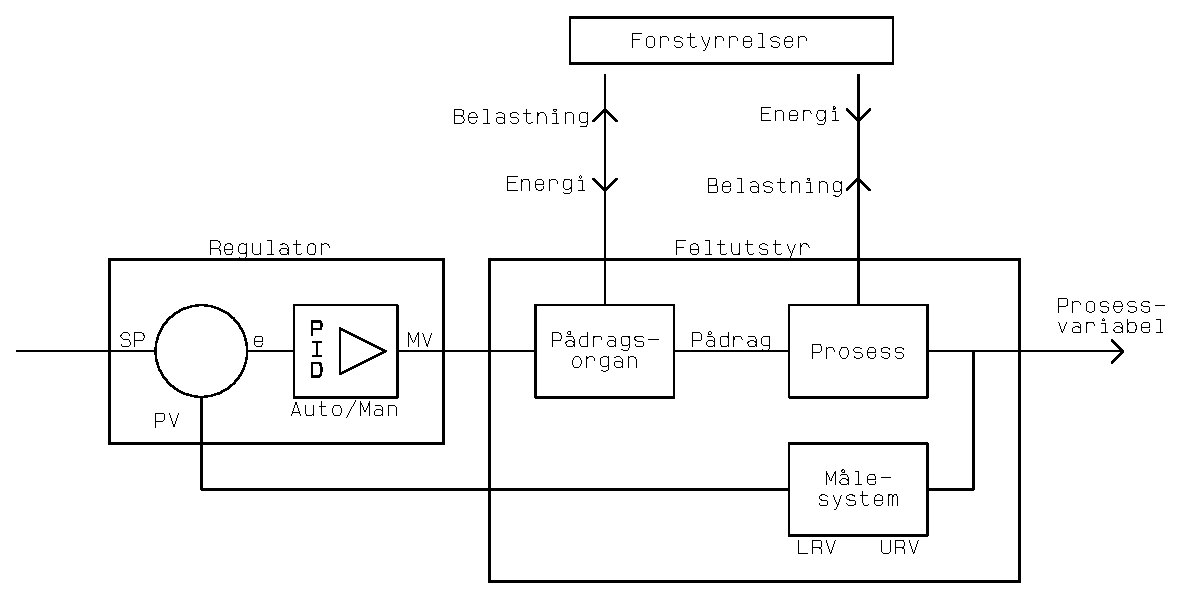
\includegraphics[height=4cm]{./regblock.eps}$$
\end{frame}
%
%Specifically, the type of feedback we are employing here to control the process is \textit{negative} or \textit{degenerative} feedback.  The term ``negative'' refers to the direction of action the control system takes in response to any measured change in the process variable.  If something happens to drive the process variable up, the control system will automatically respond in such a way as to bring the process variable back down where it belongs.  If the process variable happens to sag below setpoint, the control system will automatically act to drive the process variable back up to setpoint.  Whatever the process variable does in relation to setpoint, the control system takes the opposite (inverse, or negative) action in an attempt to stabilize it at setpoint.
%
%For example, if the unheated process fluid flow rate were to suddenly increase, the heat exchanger outlet temperature would fall due to the physics of heat transfer, but once this drop was detected by the transmitter and reported to the controller, the controller would automatically call for additional steam flow to compensate for the temperature drop, thus bringing the process variable back in agreement with the setpoint.  Ideally, a well-designed and well-tuned control loop will sense and compensate for \textit{any} change in the process or in the setpoint, the end result being a process variable value that always holds steady at the setpoint value.
%
%The unheated fluid flow rate is an example of an uncontrolled, or \textit{wild}, variable because our control system here has no ability to influence it.  This flow is also referred to as a \textit{load} because it ``loads'' or affects the process variable we are trying to stabilize.  Loads are present in nearly every controlled system, and indeed are the primary factor necessitating a control system at all.  Referring back to our heat exchanger process again, we could adequately control the operating temperature of it with just a manually-set steam control valve if only none of the other factors (steam temperature, fluid flow rate, incoming fluid temperature, etc.) ever changed!  \index{Wild variable}  \index{Load}
%
%\vskip 10pt
%
%Many types of processes lend themselves to feedback control.  Consider an aircraft autopilot system, keeping an airplane on a steady course heading despite the effects of loads such as side-winds: reading the plane's heading (process variable) from an electronic compass and using the rudder as a final control element to change the plane's ``yaw.''  An automobile's ``cruise control'' is another example of a feedback control system, with the process variable being the car's velocity, and the final control element being the engine's throttle.  The purpose of a cruise control is to maintain constant driving speed despite the influence of loads such as hills, head-winds, tail-winds, and road roughness.  Steam boilers with automatic pressure controls, electrical generators with automatic voltage and frequency controls, and water pumping systems with automatic flow controls are further examples of how feedback may be used to maintain control over certain process variables.
%
%Modern technology makes it possible to control nearly anything that may be measured in an industrial process.  This extends beyond the pale of simple pressure, level, temperature, and flow variables to include even certain chemical properties.
%
%\filbreak
%
%In municipal water and wastewater treatment systems, for example, numerous chemical quantities must be measured and controlled automatically to ensure maximum health and minimum environmental impact.  Take for instance the chlorination of treated wastewater, before it leaves the wastewater treatment facility into a large body of water such as a river, bay, or ocean.  Chlorine is added to the water to kill any residual bacteria so they do not consume oxygen in the body of water they are released to.  Too little chlorine added, and not enough bacteria are killed, resulting in a high \textit{biological oxygen demand} or \textit{BOD} in the water which will asphyxiate the fish swimming in it.  Too much chlorine added, and the chlorine itself poses a hazard to marine life.  Thus, the chlorine content must be carefully controlled at a particular setpoint, and the control system must take aggressive action if the dissolved chlorine concentration strays too low or too high: \index{Biological oxygen demand} \index{BOD} \index{Wastewater disinfection}
% 
%$$\includegraphics{cont06.eps}$$
\begin{frame}
\frametitle{Tilsetting av klor i avløpsvann før utslipp}
	$$\includegraphics[height=4cm]{cont06.eps}$$
\end{frame}
% 
%\vskip 10pt
%
%Now that we have seen the basic elements of a feedback control system, we will concentrate on the \textit{algorithms} used in the controller to maintain a process variable at setpoint.  For the scope of this topic, an ``algorithm'' is a mathematical relationship between the process variable and setpoint inputs of a controller, and the output (manipulated variable).  Control algorithms determine \textit{how} the manipulated variable quantity is deduced from PV and SP inputs, and range from the elementary to the very complex.  In the most common form of control algorithm, the so-called ``PID'' algorithm, calculus is used to determine the proper final control element action for any combination of input signals. \index{Algorithm} \index{Control algorithm}
% 
%
%
%
%
%
%
%
%%\filbreak
%%\section{Behavior of negative feedback control systems}
%
%% ADD: a new section on feedback control, exposing students to the concept and its implications
%% ADD: offsetting SP input to a feedback controller drives PV in the direction of offset
%% ADD: offsetting PV input to a feedback controller drives PV in the opposite direction of offset
%% ADD: offsetting MV output from a feedback controller has no long-term (steady-state) effect on PV
%
%
%
%
%
%
%
%
%
%
%
%
%\filbreak
%\section{Diagnosing feedback control problems}
%
%Negative feedback systems, in general, tend to cause much confusion for those first learning their fundamental principles and behaviors.  The closed-cycle ``loop'' formed by the interaction of sensing element, controller, final control element, and process means essentially that \textit{everything affects everything else}.  This is especially problematic when the feedback control system in question contains a fault and must be diagnosed.  For example, if an operator happens to notice that the process variable (as indicated by a manual measurement or by some trusted indicating instrument) is not holding to setpoint, it could be the result of a fault in \textit{any} portion of the system (sensor, controller, FCE, or even the process itself).
%
%\vskip 10pt
%
%Recall that every feedback control loop consists of four basic elements: an element that \textit{senses} the process variable (e.g. primary sensing element, transmitter), an element that \textit{decides} what how to regulate this process variable (e.g. a PID controller), an element that \textit{influences} the process variable (e.g. a control valve, motor drive, or some other final control device), and finally the process itself which \textit{reacts} to the final control device's actions:
%
%$$\includegraphics{cont98.eps}$$
%
%One of the basic diagnostic strategies for any instrumentation system is to assess whether the \textit{input value(s)} and \textit{output value(s)} correspond for each instrument.  We may apply this same strategy to each of the four elements of a feedback control ``loop'' to identify where the problem might exist.  If you encounter one of these four system portions whose output does not correspond with its input, you know that portion of the system is faulted.
%
%\filbreak
%
%\noindent
%You can check each element of your feedback control loop by comparing its input with its output to see if each element is doing what it should.  I recommend beginning with the controller (the decision-making element) because typically those values are the most easily monitored:
%
%\begin{itemize}
%\item \textbf{Decision-making:} Carefully examine the controller faceplate, looking at the values of PV, SP, and Output.  Is the controller taking appropriate action to force PV equal to SP?  In other words, is the Output signal at a value you would expect if the controller were functioning properly to regulate the process variable at setpoint?  If so, then the controller's action and tuning are most likely not at fault.  If not, then the problem definitely lies with the controller.
%\item \textbf{Sensing:} Compare the controller's displayed value for PV with the actual process variable value as indicated by local gauges, by feel, or by any other means of detection.  If there is good correspondence between the controller's PV display and the real process variable, then there probably isn't anything wrong with the measurement portion of the control loop (e.g. transmitter, impulse lines, PV signal wiring, analog input of controller, etc.).  If the displayed PV disagrees with the actual process variable value, then something is definitely wrong here.
%\item \textbf{Influencing:} Compare the controller's displayed value for Output with the actual status of the final control element.  If there is good correspondence between the controller's Output display and the FCE's status, then there probably isn't anything wrong with the output portion of the control loop (e.g. FCE, output signal wiring, analog output of controller, etc.).  If the controller Output value differs from the FCE's state, then something is definitely wrong here.
%\item \textbf{Reacting:} Compare the process variable value with the final control element's state.  Is the process doing what you would expect it to?  If so, the problem is most likely not within the process (e.g. manual valves, relief valves, pumps, compressors, motors, and other process equipment).  If, however, the process is not reacting the way you would expect it to given the final control element's state, then something is definitely awry with the process itself.
%\end{itemize}
%
%% ADD: provide multiple examples of processes with values shown for correspondence-checking.
%%     --> i02934 (maple syrup evaporation process)
%%     --> i02461 (air pressure control process)
%
%
%
%
%
%
%
%
%
%
%
%
%\filbreak
%\section{On/off control}
%
%Once while working as an instrument technician in an aluminum foundry, a mechanic asked me what it was that I did.  I began to explain my job, which was essentially to calibrate, maintain, troubleshoot, document, and modify (as needed) all automatic control systems in the facility.  The mechanic seemed puzzled as I explained the task of ``tuning'' loop controllers, especially those controllers used to maintain the temperature of large, gas-fired industrial furnaces holding many tons of molten metal.  ``Why does a controller have to be `tuned'?'' he asked.  ``All a controller does is turn the burner on when the metal's too cold, and turn it off when it becomes too hot!''
%
%In its most basic form, the mechanic's assessment of the control system was correct: to turn the burner on when the process variable (molten metal temperature) drops below setpoint, and turn it off when it rises above setpoint.  However, the actual algorithm is much more complex than that, finely adjusting the burner intensity according to the amount of \textit{error} between PV and SP, the amount of time the error has accumulated, and the rate-of-change of the error over time.  In his casual observation of the furnace controllers, though, he had noticed nothing more than the full-on/full-off action of the controller.
%
%The technical term for a control algorithm that merely checks for the process variable exceeding or falling below setpoint is \textit{on/off control}.  In colloquial terms, it is known as \textit{bang-bang} control, since the manipulated variable output of the controller rapidly switches between fully ``on'' and fully ``off'' with no intermediate state.  Control systems this crude usually provide very imprecise control of the process variable.  Consider our example of the shell-and-tube heat exchanger, if we were to implement simple on/off control\footnote{To be precise, this form of on/off control is known as \textit{differential gap} because there are two setpoints with a gap in between.  While on/off control is possible with a single setpoint (FCE on when below setpoint and off when above), it is usually not practical due to the frequent cycling of the final control element.}: \index{On-off control} \index{Bang-bang control}
%
\begin{frame}
	\frametitle{Av/På regulering}

	
	$$\includegraphics[height=4cm]{cont07.eps}$$
\end{frame}



% 
%As you can see, the degree of control is rather poor.  The process variable ``cycles'' between the upper and lower setpoints (USP and LSP) without ever stabilizing at the setpoint, because that would require the steam valve to be position somewhere \textit{between} fully closed and fully open.  
%
%This simple control algorithm may be adequate for temperature control in a house, but not for a sensitive chemical process!  Can you imagine what it would be like if an automobile's cruise control system relied on this algorithm?  Not only is the lack of precision a problem, but the frequent cycling of the final control element may contribute to premature failure due to mechanical wear.  In the heat exchanger scenario, thermal cycling (hot-cold-hot-cold) will cause metal fatigue in the tubes, resulting in a shortened service life.  Furthermore, every excursion of the process variable above setpoint is wasted energy, because the process fluid is being heated to a greater temperature than what is necessary.
%
%Clearly, the only practical answer to this dilemma is a control algorithm able to \textit{proportion} the final control element rather than just operate it at zero or full effect (the control valve fully closed or fully open).  This, in its simplest form, is called \textit{proportional control}. \index{Proportional control}
% 
%
%
%
%
%
%\filbreak
%\section{Proportional-only control}
%
%Imagine a liquid-level control system for a vessel, where the position of a level-sensing float directly sets the stem position of a control valve.  As the liquid level rises, the valve opens up proportionally:
%
%$$\includegraphics{cont76.eps}$$
\begin{frame}
	\frametitle{Proporsjonal regulator}

	
	$$\includegraphics[height=4cm]{cont76.eps}$$
\end{frame}









	
%
%Despite its crude mechanical nature, this \textit{proportional} control system would in fact help regulate the level of liquid inside the process vessel.  If an operator wished to change the ``setpoint'' value of this level control system, he or she would have to adjust the coupling between the float and valve stems for more or less distance between the two.  Increasing this distance (lengthening the connection) would effectively raise the level setpoint, while decreasing this distance (shortening the connection) would lower the setpoint.
%
%\filbreak
%
%We may generalize the proportional action of this mechanism to describe \textit{any} form of controller where the output is a direct function of process variable (PV) and setpoint (SP):
%
\begin{frame}
	\frametitle{Formel for proporsjonal regulator}

$$MV = K_p e + bias$$

\vskip 5pt 
%
%\noindent
%Where,
%
$MV$ = Regulatorens utgang
\vskip 5pt 
%
	$e$ = Error(avvik) (Forskjellen mellom PV og SP)
\vskip 5pt 
%
$K_p$ = Proporsjonalforsterkning
\vskip 5pt 
%
$b$ = Bias
\vskip 5pt 
\end{frame}
\begin{frame}
	\frametitle{BIAS (offset)}

	$$\includegraphics[height=6cm]{cont12.eps}$$
\end{frame}
%
%\vskip 10pt
%
%A new term introduced with this formula is $e$, the ``error'' or difference between process variable and setpoint.  Error may be calculated as SP$-$PV or as PV$-$SP, depending on whether or not the controller must produce an \textit{increasing} output signal in response to an increase in the process variable (``direct'' acting), or output a \textit{decreasing} signal in response to an increase in the process variable (``reverse'' acting):  \index{Error, controller}  \index{Direct-acting controller}  \index{Reverse-acting controller}  \index{Action, controller}  \index{Controller action, direct vs. reverse}  
%
\begin{frame}
	\frametitle{Direkte eller reverserende regulator}

$$m = K_p (\hbox{PV} - \hbox{SP}) + b \hskip 30pt \hbox{(Direct-acting proportional controller)}$$
%

\vskip 5pt 
$$m = K_p(\hbox{SP} - \hbox{PV}) + b \hskip 30pt \hbox{(Reverse-acting proportional controller)}$$

\vskip 5pt 
%$$\includegraphics{cont77.eps}$$
	$$\includegraphics[height=4cm]{cont77.eps}$$
\end{frame}

%
%The optional ``+'' and ``$-$'' symbols clarify the effect each input has on the controller output: a ``$-$'' symbol representing an \textit{inverting} effect and a ``+'' symbol representing a \textit{noninverting} effect.  When we say that a controller is ``direct-acting'' or ``reverse-acting'' we are referring to it reaction to the PV signal, therefore the output signal from a ``direct-acting'' controller goes in the same direction as the PV signal and the output from a ``reverse-acting'' controller goes in the opposite direction of its PV signal.  It is important to note, however, that the response to a change in setpoint (SP) will yield the \textit{opposite} response as does a change in process variable (PV): a rising SP will drive the output of a direct-acting controller \textit{down} while a rising SP drives the output of a reverse-acting controller \textit{up}.  ``+'' and ``$-$'' symbols explicitly show the effect both inputs have on the controller output, helping to avoid confusion when analyzing the effects of PV changes versus the effects of SP changes.
%
%\filbreak
%
%The direction of action required of the controller is determined by the nature of the process, transmitter, and final control element.  In the case of the crude mechanical level controller, the action needs to be \textit{direct} so that a greater liquid level will result in a further-open control valve to drain the vessel faster.  In the case of the automated heat exchanger shown earlier, we are assuming that an increasing output signal sent to the control valve results in increased steam flow, and consequently higher temperature, so our controller will need to be reverse-acting (i.e. an increase in measured temperature results in a decrease in output signal; error calculated as SP$-$PV): 
\begin{frame}
	\frametitle{Direkte eller reverserende regulator?}

	$$\includegraphics[height=6cm]{cont04.eps}$$
\end{frame}
%
%$$\includegraphics{cont04.eps}$$
%
%After the error has been calculated, the controller then multiplies the error signal by a constant value called the \textit{gain}, which is programmed into the controller.  The resulting figure, plus a ``bias'' quantity, becomes the output signal sent to the valve to proportion it.  The ``gain'' value is exactly what it seems to be for anyone familiar with electronic amplifier circuits: a ratio of output to input.  In this case, the gain of a proportional controller is the ratio of output signal change to input signal change, or how \textit{aggressive} the controller reacts to changes in input (PV or SP). \index{Gain, controller} \index{Controller gain}
%
%To give a numerical example, a loop controller set to have a gain of 4 will change its output signal by 40\% if it sees an input change of 10\%: the ratio of output change to input change will be 4:1.  Whether the input change comes in the form of a setpoint adjustment, a drift in the process variable, or some combination of the two does not matter to the magnitude of the output change.
%
%The bias value of a proportional controller is simply the value of its output whenever process variable happens to be equal to setpoint (i.e. a condition of zero \textit{error}).  Without a bias term in the proportional control formula, the valve would always return to a fully shut (0\%) condition if ever the process variable reached the setpoint value.  The bias term allows the final control element to achieve a non-zero state at setpoint.
%
%\vskip 10pt
%
%%\filbreak
%
%%If the $m = K_p e + b$ proportional controller formula resembles the standard slope-intercept form of linear equation ($y = mx + b$), it is more than coincidence.  Often, the response of a proportional controller is shown graphically as a line, the slope of the line representing gain and the y-intercept of the line representing the output bias point, or what value the output signal will be when there is no error (PV precisely equals SP):
% 
\begin{frame}
	\frametitle{For stor prporsjonalforsterkning}

	$$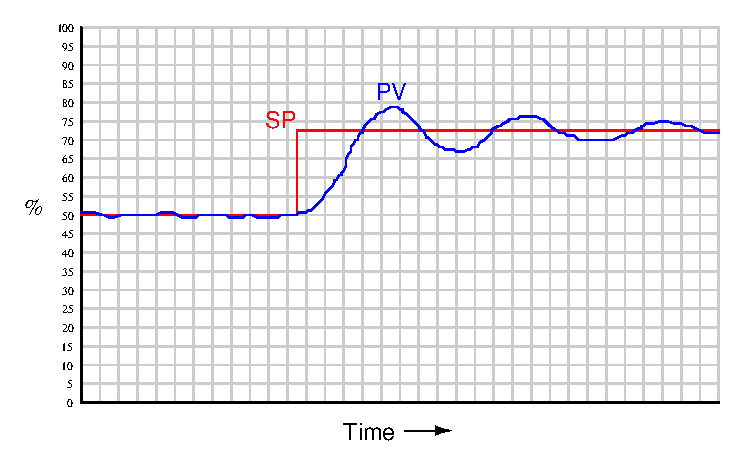
\includegraphics[height=8cm]{cont09.eps}$$
\end{frame}

%%$$\includegraphics{cont08.eps}$$ 
%
%%In this graph the bias value is 50\% and the gain of the controller is 1.  Changing the bias value ($b$) of the controller shifts the line up or down.  Changing the gain value ($K_p$) alters the slope of the line for more or less aggressive control action.
%
%%\vskip 10pt
%
%If the controller could be configured for infinite gain, its response would duplicate on/off control.  That is, \textit{any} amount of error will result in the output signal becoming ``saturated'' at either 0\% or 100\%, and the final control element will simply turn on fully when the process variable drops below setpoint and turn off fully when the process variable rises above setpoint.  Conversely, if the controller is set for zero gain, it will become completely unresponsive to changes in either process variable \textit{or} setpoint: the valve will hold its position at the bias point no matter what happens to the process.
%
%Obviously, then, we must set the gain somewhere between infinity and zero in order for this algorithm to function any better than on/off control.  Just how much gain a controller needs to have depends on the process and all the other instruments in the control loop.  
%
%\vskip 10pt
%
%If the gain is set too high, there will be oscillations as the PV converges on a new setpoint value:
% 
%$$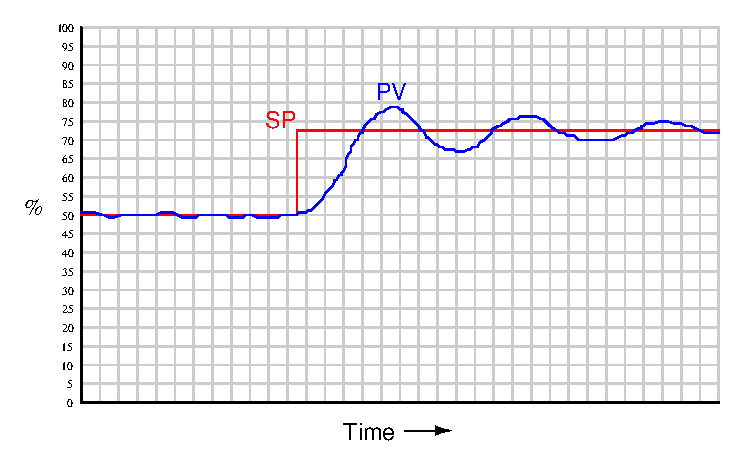
\includegraphics{cont09.eps}$$
\begin{frame}
	\frametitle{For lav proporsjonalforsterkning}

	$$\includegraphics[height=8cm]{cont10.eps}$$
\end{frame}

%
%\filbreak
%
%If the gain is set too low, the process response will be stable under steady-state conditions but relatively slow to respond to changes in setpoint, as shown in the following trend recording:
% 
%$$\includegraphics{cont10.eps}$$
%
%A characteristic deficiency of proportional control action, exacerbated with low controller gain values, is a phenomenon known as \textit{proportional-only offset} where the PV never fully reaches SP.  A full explanation of proportional-only offset is too lengthy for this discussion and will be presented in a subsequent section of the book, but may be summarized here simply by drawing attention to the proportional controller equation which tells us the output always returns to the bias value when PV reaches SP (i.e. $m = b$ when PV = SP).  If anything changes in the process to require a different output value than the bias ($b$) to stabilize the PV, an error between PV and SP \textit{must} develop to drive the controller output to that necessary output value.  This means it is only by chance that the PV will settle precisely at the SP value -- most of the time, the PV will deviate from SP in order to generate an output value sufficient to stabilize the PV and prevent it from drifting.  This persistent error, or offset, worsens as the controller gain is reduced.  Increasing controller gain causes this offset to decrease, but at the expense of oscillations.
%
%\filbreak
%
%With proportional-only control, the choice of gain values is really a compromise between excessive oscillations and excessive offset.  A well-tuned proportional controller response is shown here:
% 
\begin{frame}
	\frametitle{Passelig proporsjonalforsterkning}

	$$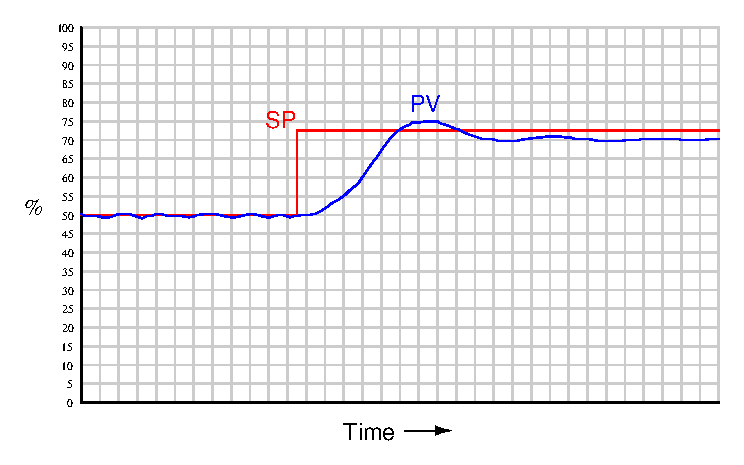
\includegraphics[height=8cm]{cont11.eps}$$
\end{frame}

%$$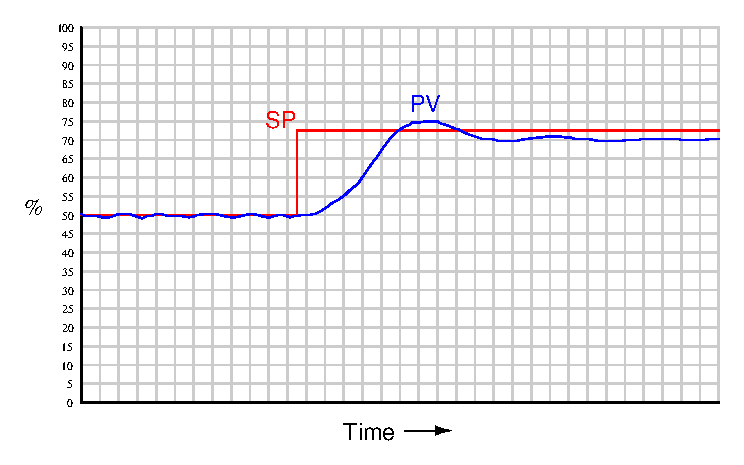
\includegraphics{cont11.eps}$$
%
%An unnecessarily confusing aspect of proportional control is the existence of two completely different ways to express controller proportionality.  In the proportional-only equation shown earlier, the degree of proportional action was specified by the constant $K_p$, called \textit{gain}.  However, there is another way to express the sensitivity of proportional action, and that is to state the percentage of error change necessary to make the output ($m$) change by 100\%.  Mathematically, this is the inverse of gain, and it is called \textit{proportional band} (PB):  \index{Proportional band}
%
\begin{frame}
	\frametitle{Proportionalbånd vs Proportionalforsterkning}

$$K_p = {100\% \over \hbox{PB}} \hskip 30pt \hbox{PB} = {100\% \over K_p}$$
\end{frame}

%
%Gain is always specified as a unitless value\footnote{In electronics, the unit of \textit{decibels} is commonly used to express gains.  Thankfully, the world of process control was spared the introduction of decibels as a unit of measurement for controller gain.  The last thing we need is a \textit{third} way to express the degree of proportional action in a controller!}, whereas proportional band is always specified as a percentage.  For example, a gain value of 2.5 is equivalent to a proportional band value of 40\%, because the error input to this controller must change by 40\% in order to make the output change a full 100\%.
%
%\filbreak
%
%Due to the existence of these two completely opposite conventions for specifying proportional action, you may see the proportional term of the control equation written differently depending on whether the author assumes the use of gain or the use of proportional band:
%
%% No blank lines allowed between lines of an \halign structure!
%% I use comments (%) instead, so that TeX doesn't choke.
%
%$$\vbox{\offinterlineskip
%\halign{\strut
%\quad\hfil # \ \hfil & 
%\quad\hfil # \ \hfil \cr
%%
%% First row
%$K_p$ = gain & PB = proportional band \cr
%%
%\noalign{\vskip 5pt}
%%
%% Another row
%$K_p e$  &  ${1 \over \hbox{PB}} e$ \cr
%%
%%\noalign{\hrule}
%} % End of \halign 
%}$$ % End of \vbox
%
%Many modern digital electronic controllers allow the user to conveniently select the unit they wish to use for proportional action.  However, even with this ability, anyone tasked with adjusting a controller's ``tuning'' values may be required to translate between gain and proportional band, especially if certain values are documented in a way that does not match the unit configured for the controller.  
%
%When you communicate the proportional action setting of a process controller, you should always be careful to specify either ``gain'' or ``proportional band'' to avoid ambiguity.  \textit{Never} simply say something like, ``The proportional setting is twenty,'' for this could mean either:
%
%\begin{itemize}
%\item Proportional band = 20\%; Gain = 5 \hskip 20pt \textit{. . . or . . .}
%\item Gain = 20; Proportional band = 5\%
%\end{itemize}
%
%As you can see here, the real-life difference in controller response to an input disturbance (wave) depending on whether it has a proportional band of 20\% or a gain of 20 is quite dramatic:
%
\begin{frame}
	\frametitle{Eksempel}

	$$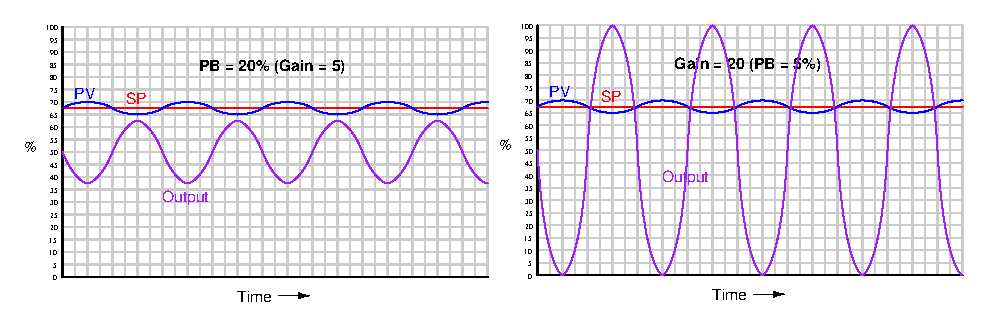
\includegraphics[width=1\textwidth]{cont87.eps}$$
\end{frame}

%$$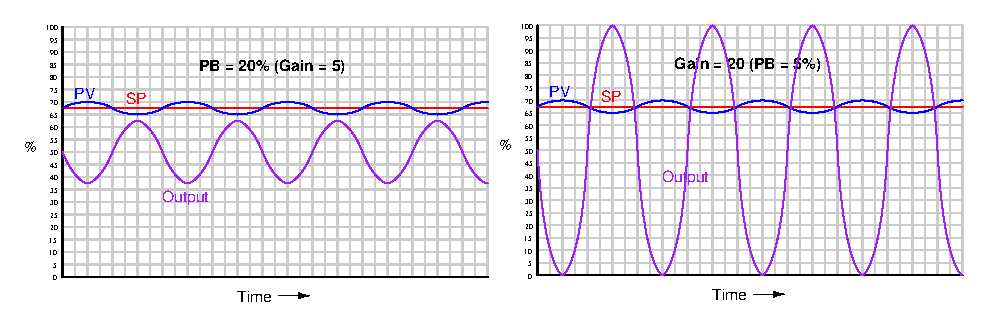
\includegraphics{cont87.eps}$$
%
%
%
%
%
%
%
%
%
%
%\filbreak
%\section{Proportional-only offset}
%
%A fundamental limitation of proportional control has to do with its response to changes in setpoint and changes in process \textit{load}.  A ``load'' in a controlled process is any variable not controlled by the loop controller which nevertheless affects the process variable the controller is trying to regulate.  In other words, a ``load'' is any factor the loop controller must compensate for while maintaining the process variable at setpoint. \index{Load}
%
%In our hypothetical heat exchanger system, the temperature of the incoming process fluid is an example of a load:
%

%$$\includegraphics{cont12.eps}$$
%
%If the incoming fluid temperature were to suddenly decrease, the immediate effect this would have on the process would be to decrease the outlet temperature (which is the temperature we are trying to maintain at a steady value).  It should make intuitive sense that a colder incoming fluid will require more heat input to raise it to the same outlet temperature as before.  If the heat input remains the same (at least in the immediate future), this colder incoming flow must make the outlet flow colder than it was before.  Thus, incoming feed temperature has an impact on the outlet temperature whether we like it or not, and the control system must compensate for these unforeseen and uncontrolled changes.  This is precisely the definition of a ``load'': a burden\footnote{One could argue that the presence of loads actually \textit{justifies} a control system, for if there were no loads, there would be nothing to compensate for, and therefore no need for an automatic control system at all!  In the total absence of loads, a manually-set final control element would be enough to hold most process variables at setpoint.} on the control system.
%
%Of course, it is the job of the controller to counteract any tendency for the outlet temperature to stray from setpoint, but as we shall soon see this cannot be perfectly achieved with proportional control alone.  
%
%\vskip 10pt
%
%Let us perform a ``thought experiment'' to demonstrate this phenomenon of proportional-only offset.  Imagine the controller has been controlling outlet temperature exactly at setpoint (PV = SP), and then suddenly the inlet feed temperature drops and remains colder than before.  Recall that the equation for a reverse-acting proportional controller is as follows:  \index{Thought experiment}  \index{Problem-solving technique: thought experiment}
%

%\vskip 10pt
%
%The introduction of colder feed fluid to the heat exchanger makes the outlet temperature (PV) begin to fall.  As the PV falls, the controller calculates a positive error (SP $-$ PV).  This positive error, when multiplied by the controller's gain value, drives the output to a greater value.  This opens up the steam valve, adding more heat to the exchanger.
%
%As more heat is added, the rate of temperature drop slows down.  The further the PV drops, the more the steam valve opens, until enough additional heat is being added to the heat exchanger to maintain a constant outlet temperature.  However, this new stable PV value will be less than it was prior to the introduction of colder feed (i.e. less than the SP).  In fact, the controller's automatic action can \textit{never} return the PV to its original (SP) value so long as the feed remains colder than before.  The reason for this is that a greater flow of steam is necessary to balance a colder feed coming in, and the only way a proportional controller is ever going to automatically drive the steam valve to this greater-flow position is if an error develops between PV and SP.  Thus, an \textit{offset} inevitably develops between PV and SP due to the load (colder feed).
%
%We may prove the inevitability of this offset another way: imagine somehow that the PV did actually return to the SP value despite the colder feed fluid (remaining colder).  If this happened, the steam valve would also return to its former throttling position where it was before the feed temperature dropped.  However, we know that this former position will not allow enough steam through to the exchanger to overcome the colder feed -- if it did, the PV never would have decreased to begin with!  A further-open valve is precisely what we need to stabilize the PV given this colder feed, yet the only way the proportional-only controller can achieve this is if the PV actually falls below SP.
%
%To summarize: the only way a proportional-only controller can automatically generate a new output value ($m$) is if the PV deviates from SP.  Therefore, load changes (requiring new output values to compensate) force the PV to deviate from SP.
%
%\vskip 10pt
%
%\filbreak
%
%Another ``thought experiment'' may be helpful to illustrate the phenomenon of proportional-only offset.  Imagine building your own cruise control system for your automobile based on the proportional-only equation: the engine's throttle position is a function of the difference between PV (road speed) and SP (the desired ``target'' speed).  Let us further suppose that you carefully adjust the bias value of your cruise control system to achieve PV = SP on level ground at a speed of 70 miles per hour (70\% on a 0 to 100 MPH speedometer scale), with the throttle at a position of 40\%, and a gain ($K_p$) of 2:
%
%$$m = K_p (\hbox{SP} - \hbox{PV}) + b$$
%
%$$40\% = 2 (70 - 70) + 40\%$$
%
%Imagine now that after cruising precisely at setpoint (70\% = 70 MPH), the road begins to incline uphill for several miles.  This, obviously, is a load on the cruise control system.  With the cruise control disengaged, the automobile would slow down because the same throttle position (40\%) sufficient to maintain setpoint (70 MPH) on level ground is not enough power to maintain that same setpoint on an incline.  
%
%With the cruise control engaged, the engine throttle will automatically open further as speed drops.  At a speed of 69 MPH, the throttle opens up to 42\%.  At a speed of 68 MPH, the throttle opens up to 44\%.  Every drop in speed of 1 MPH results in a 2\% further-open throttle to send more power to the wheels.
%
%Suppose the demands of this particular inclined road require a 50\% throttle position for this automobile to maintain a constant speed.  In order for your proportional-only cruise control system to deliver this necessary 50\% throttle position, the speed will have to ``droop'' by 5 MPH below setpoint:
%
%$$m = K_p (\hbox{SP} - \hbox{PV}) + b$$
%
%$$50\% = 2 (70 - 65) + 40\%$$
%
%There is simply no other way for your proportional-only controller to automatically achieve the requisite 50\% throttle position aside from letting the speed sag below setpoint by 5\% (5 MPH).  Given this fact, the only way the proportional-only cruise control will ever return the speed to setpoint (70 MPH) is if and when the load conditions change to allow for a lesser throttle position of 40\%.  So long as the load demands a different throttle position than the bias value, the speed \textit{must} deviate from the setpoint value of 70 MPH.
%
%\vskip 10pt
%
%This necessary error developing between PV and SP is called \textit{proportional-only offset}, sometimes called \textit{droop}.  The amount of droop depends on how severe the load change is, and how aggressive the controller responds (i.e. how much gain it has).  The term ``droop'' is very misleading, as it is possible for the error to develop the other way (i.e. the PV might rise above SP due to a load change!).  Imagine the opposite load-change scenario in our steam heat exchanger process, where the incoming feed temperature suddenly \textit{rises} instead of falls.  If the controller was controlling exactly at setpoint before this upset, the final result will be an outlet temperature that settles at some point \textit{above} setpoint, enough so the controller is able to pinch the steam valve far enough closed to stop any further rise in temperature. \index{Proportional-only offset} \index{Droop}
%
%Proportional-only offset also occurs as a result of setpoint changes.  We could easily imagine the same sort of effect following an operator's increase of setpoint for the temperature controller on the heat exchanger.  After increasing the setpoint, the controller immediately increases the output signal, sending more steam to the heat exchanger.  As temperature rises, though, the proportional algorithm causes the output signal to decrease.  When the rate of heat energy input by the steam equals the rate of heat energy carried away from the heat exchanger by the heated fluid (a condition of \textit{energy balance}), the temperature stops rising.  This new equilibrium temperature will not be at setpoint, assuming the temperature was holding at setpoint prior to the human operator's setpoint increase.  The new equilibrium temperature indeed \textit{cannot} ever achieve any setpoint value higher than the one it did in the past, for if the error ever returned to zero (PV = SP), the steam valve would return to its old position, which we know would be insufficient to raise the temperature of the heated fluid to a new value.
%
%\vskip 10pt
%
%An example of proportional-only control in the context of electronic power supply circuits is the following opamp voltage regulator, used to stabilize voltage to a load with power supplied by an unregulated voltage source:
%
%$$\includegraphics{cont68.eps}$$
%
%In this circuit, a zener diode establishes a ``reference'' voltage (which may be thought of as a ``setpoint'' for the controlling opamp to follow).  The operational amplifier acts as the proportional-only controller, sensing voltage at the load (PV), and sending a driving output voltage to the base of the power transistor to keep load voltage constant despite changes in the supply voltage or changes in load current (both ``loads'' in the process-control sense of the word, since they tend to influence voltage at the load circuit without being under the control of the opamp).
%
%If everything functions properly in this voltage regulator circuit, the load's voltage will be stable over a wide range of supply voltages and load currents.  However, the load voltage cannot ever \textit{precisely} equal the reference voltage established by the zener diode, even if the operational amplifier (the ``controller'') is without defect.  The reason for this incapacity to perfectly maintain ``setpoint'' is the simple fact that in order for the opamp to generate any output signal at all, there \textit{absolutely must be} a differential voltage between the two input terminals for the amplifier to amplify.  Operational amplifiers (ideally) generate an output voltage equal to the enormously high gain value ($A_V$) multiplied by the difference in input voltages (in this case, $V_{ref} - V_{load}$).  If $V_{load}$ (the ``process variable'') were to ever achieve equality with $V_{ref}$ (the ``setpoint''), the operational amplifier would experience absolutely no differential input voltage to amplify, and its output signal driving the power transistor would fall to zero.  Therefore, there must always exist some \textit{offset} between $V_{load}$ and $V_{ref}$ (between process variable and setpoint) in order to give the amplifier some input voltage to amplify.
%
%The amount of offset is ridiculously small in such a circuit, owing to the enormous gain of the operational amplifier.  If we take the opamp's transfer function to be $V_{out} = A_V (V_{(+)} - V_{(-)})$, then we may set up an equation predicting the load voltage as a function of reference voltage (assuming a constant 0.7 volt drop between the base and emitter terminals of the transistor):
%
%$$V_{out} = A_V(V_{(+)} - V_{(-)})$$
%
%$$V_{out} = A_V(V_{ref} - V_{load})$$
%
%$$V_{load} + 0.7 = A_V(V_{ref} - V_{load})$$
%
%$$V_{load} + 0.7 = A_V V_{ref} - A_V V_{load}$$
%
%$$V_{load} + A_V V_{load} = A_V V_{ref} - 0.7$$
%
%$$(A_V + 1) V_{load} = A_V V_{ref} - 0.7$$
%
%$$V_{load} = {{A_V V_{ref} - 0.7} \over {A_V + 1}}$$
%
%If, for example, our zener diode produced a reference voltage of 5.00000 volts and the operational amplifier had an open-loop voltage gain of 250000, the load voltage would settle at a theoretical value of 4.9999772 volts: just barely below the reference voltage value.  If the opamp's open-loop voltage gain were much less -- say only 100 -- the load voltage would only be 4.94356 volts.  This still is quite close to the reference voltage, but definitely not as close as it would be with a greater opamp gain!
%
%\vskip 10pt
%
%Clearly, then, we can minimize proportional-only offset by increasing the gain of the process controller gain (i.e. decreasing its proportional band).  This makes the controller more ``aggressive'' so it will move the control valve further for any given change in PV or SP.  Thus, not as much error needs to develop between PV and SP to move the valve to any new position it needs to go.  However, too much controller gain makes the control system unstable: at best it will exhibit residual oscillations after setpoint and load changes, and at worst it will oscillate out of control altogether.  Extremely high gains work well to minimize offset in operational amplifier circuits, only because time delays are negligible between output and input.  In applications where large physical processes are being controlled (e.g. furnace temperatures, tank levels, gas pressures, etc.) rather than voltages across small electronic loads, such high controller gains would be met with debilitating oscillations.
%
%If we are limited in how much gain we can program in to the controller, how do we minimize this offset?  One way is for a human operator to periodically place the controller in manual mode and move the control valve just a little bit more so the PV once again reaches SP, then place the controller back into automatic mode.  In essence this technique adjusts the ``Bias'' term of the controller equation.  The disadvantage of this technique is rather obvious: it requires human intervention.  What is the point of having an automation system requiring periodic human intervention to maintain setpoint?
%
%A more sophisticated method for eliminating proportional-only offset is to add a different control action to the controller: one that takes action based on the amount of error between PV and SP and the amount of time that error has existed.  We call this control mode \textit{integral}, or \textit{reset}.
%
%
%
%
%
%%\filbreak
%%\subsection{Practical examples of proportional-only offset}
%
%
%
%
%
%
%
%\filbreak
%\section{Integral (reset) control}
%
%Imagine a liquid-level control system for a vessel, where the position of a level-sensing float sets the position of a potentiometer, which then sets the \textit{speed} of a motor-actuated control valve.  If the liquid level is above setpoint, the valve continually opens up; if below setpoint, the valve continually closes off:
%
\begin{frame}
	\frametitle{I-leddet}

	$$\includegraphics[height=7cm]{cont78.eps}$$
\end{frame}

%$$\includegraphics{cont78.eps}$$
%
%Unlike the \textit{proportional} control system where valve position was a direct function of float position, this control system sets the \textit{speed} of the motor-driven valve according to the float position.  The further away from setpoint the liquid level is, the \textit{faster} the valve moves open or closed.  In fact, the only time the valve will ever halt its motion is when the liquid level is precisely at setpoint; otherwise, the control valve will be in constant motion.
%
%This control system does its job in a very different manner than the all-mechanical float-based proportional control system illustrated previously.  Both systems are capable of regulating liquid level inside the vessel, but they take very different approaches to doing so.  One of the most significant differences in control behavior is how the proportional system would inevitably suffer from \textit{offset} (a persistent error between PV and SP), whereas this control system actively works at all times to eliminate offset.  The motor-driven control valve literally does not rest until all error has been eliminated!
%
%\vskip 10pt
%
%\filbreak
%
%Instead of characterizing this control system as \textit{proportional}, we call it \textit{integral}\footnote{An older term for this mode of control is \textit{floating}, which I happen to think is particularly descriptive.  With a ``floating'' controller, the final control element continually ``floats'' to whatever value it must in order to completely eliminate offset.} in honor of the calculus principle (``integration'') whereby small quantities are accumulated over some span to form a total.  Don't let the word ``calculus'' scare you!  You are probably already familiar with the concept of numerical integration even though you may have never heard of the term before. \index{Integral control action}  \index{Reset control action}  \index{Floating control action}
%
%Calculus is a form of mathematics dealing with \textit{changing} variables, and how rates of change relate between different variables.  When we ``integrate'' a variable with respect to time, what we are doing is \textit{accumulating} that variable's value as time progresses.  Perhaps the simplest example of this is a vehicle odometer, accumulating the total distance traveled by the vehicle over a certain time period.  This stands in contrast to a speedometer, indicating the rate of distance traveled \textit{per} unit of time.
%
%Imagine a car moving along at exactly 30 miles per hour.  How far will this vehicle travel after 1 hour of driving this speed?  Obviously, it will travel 30 miles.  Now, how far will this vehicle travel if it continues for another 2 hours at the exact same speed?  Obviously, it will travel 60 more miles, for a total distance of 90 miles since it began moving.  If the car's speed is a constant, calculating total distance traveled is a simple matter of multiplying that speed by the travel time.
%
%The odometer mechanism that keeps track of the mileage traveled by the car may be thought of as \textit{integrating} the speed of the car with respect to time.  In essence, it is multiplying speed times time continuously to keep a running total of how far the car has gone.  When the car is traveling at a high speed, the odometer ``integrates'' at a faster rate.  When the car is traveling slowly, the odometer ``integrates'' slowly.
% 
%If the car travels in reverse, the odometer will decrement (count down) rather than increment (count up) because it sees a negative quantity for speed\footnote{At least the old-fashioned mechanical odometers would.  Modern cars use a pulse detector on the driveshaft which cannot tell the difference between forward and reverse, and therefore their odometers always increment.  Shades of the movie \textit{Ferris Bueller's Day Off.}}.  The rate at which the odometer decrements depends on how fast the car travels in reverse.  When the car is stopped (zero speed), the odometer holds its reading and neither increments nor decrements.
%
%\vskip 10pt
%
%Now let us return to the context of an automated process to see how this calculus principle works inside a process controller.  Integration is provided either by a pneumatic mechanism, an electronic opamp circuit, or by a microprocessor executing a digital integration algorithm.  The variable being integrated is \textit{error} (the difference between PV and SP) over time.  Thus the integral mode of the controller ramps the output either up or down over time in response to the amount of error existing between PV and SP, and the sign of that error.  We saw this ``ramping'' action in the behavior of the liquid level control system using a motor-driven control valve commanded by a float-positioned potentiometer: the valve stem continuously moves so long as the liquid level deviates from setpoint.  The reason for this ramping action is to increase or decrease the output \textit{as far as it is necessary} in order to completely eliminate any error and force the process variable to precisely equal setpoint.  Unlike proportional action, which simply moves the output an amount proportional to any change in PV or SP, integral control action never stops moving the output until all error is eliminated.  \index{Error, controller}
%
%\vskip 10pt
%
%\filbreak
%
%If proportional action is defined by the error telling the output how \textit{far} to move, integral action is defined by the error telling the output how \textit{fast} to move.  One might think of integral as being how ``impatient'' the controller is, with integral action constantly ramping the output as far as it needs to go in order to eliminate error.  Once the error is zero (PV = SP), of course, the integral action stops ramping, leaving the controller output (valve position) at its last value just like a stopped car's odometer holds a constant value. 
%
%If we add an integral term to the controller equation, we get something that looks like this\footnote{The equation for a proportional + integral controller is often written without the bias term ($b$), because the presence of integral action makes it unnecessary.  In fact, if we let the integral term completely replace the bias term, we may consider the integral term to be a self-\textit{resetting} bias.  This, in fact, is the meaning of the word ``reset'' in the context of PID controller action: the ``reset'' term of the controller acts to eliminate offset by continuously adjusting (resetting) the bias as necessary.}:
%
\begin{frame}
	\frametitle{Formel for PI-regulator}


$$MV = K_p e + {1 \over T_i} \int e \> dt + b$$
\vskip 5pt 
Where,
\vskip 5pt 
$MV$ = Controller output
\vskip 5pt 
$K_p$ = Proportional gain
\vskip 5pt 
$T_i$ = Integral time constant (minutes)
\vskip 5pt 
$t$ = Time
\vskip 5pt 
$b$ = Bias
\vskip 5pt 

\end{frame}
%The most confusing portion of this equation for those new to calculus is the part that says ``$\int e \> dt$''.  The integration symbol (looks like an elongated letter ``S'') tells us the controller will accumulate (``sum'') multiple products of error ($e$) over tiny slices of time ($dt$).  Quite literally, the controller multiplies error by time (for very short segments of time, $dt$) and continuously adds up all those products to contribute to the output signal which then drives the control valve (or other final control element).  The integral time constant ($\tau_i$) is a value set by the technician or engineer configuring the controller, proportioning this cumulative action to make it more or less aggressive over time.
%
%\vskip 10pt
%
%To see how this works in a practical sense, let's imagine how a proportional + integral controller would respond to the scenario of a heat exchanger whose inlet temperature suddenly dropped.  As we saw with proportional-only control, an inevitable offset occurs between PV and SP with changes in load, because an error \textit{must} develop if the controller is to generate the different output signal value necessary to halt further change in PV.  We called this effect \textit{proportional-only offset}.   \index{Proportional-only offset}
%
%Once this error develops, though, integral action begins to work.  Over time, a larger and larger quantity accumulates in the integral mechanism (or register) of the controller due to the persistent error between PV and SP.  That accumulated value adds to the controller's output, driving the steam control valve further and further open.  This, of course, adds heat at a faster rate to the heat exchanger, which causes the outlet temperature to rise.  As the temperature re-approaches setpoint, the error becomes smaller and thus the integral action proceeds at a slower rate (like a car's odometer incrementing at a slower rate as the car's speed decreases).  So long as the PV is below SP (the outlet temperature is still too cool), the controller will continue to integrate upwards, driving the control valve further and further open.  Only when the PV rises to exactly meet SP does integral action finally rest, holding the valve at a steady position.  Integral action tirelessly works to eliminate any offset between PV and SP, thus neatly eliminating the offset problem experienced with proportional-only control action.
%
%\vskip 10pt
%
%As with proportional action, there are (unfortunately) two completely opposite ways to specify the degree of integral action offered by a controller.  One way is to specify integral action in terms of \textit{minutes} or \textit{minutes per repeat}.  A large value of ``minutes'' for a controller's integral action means a less aggressive integral action over time, just as a large value for proportional band means a less aggressive proportional action.  The other way to specify integral action is the inverse: how many \textit{repeats per minute}, equivalent to specifying proportional action in terms of gain  (large value means aggressive action).  For this reason, you will sometimes see the integral term of a PID equation written differently:
%
%% No blank lines allowed between lines of an \halign structure!
%% I use comments (%) instead, so that TeX doesn't choke.
%
%$$\vbox{\offinterlineskip
%\halign{\strut
%\quad\hfil # \ \hfil & 
%\quad\hfil # \ \hfil \cr
%%
%% First row
%$\tau_i$ = minutes per repeat & $K_i$ = repeats per minute \cr
%%
%\noalign{\vskip 5pt}
%%
%% Another row
%${1 \over \tau_i} \int e \> dt$  &  $K_i \int e \> dt$ \cr
%%
%%\noalign{\hrule}
%} % End of \halign 
%}$$ % End of \vbox
%
%Many modern digital electronic controllers allow the user to select the unit they wish to use for integral action, just as they allow a choice between specifying proportional action as gain or as proportional band.
%
%\vskip 10pt
%
%Integral is a highly effective mode of process control.  In fact, some processes respond so well to integral controller action that it is possible to operate the control loop on integral action alone, without proportional.  Typically, though, process controllers implement some form of proportional plus integral (``PI'') control.
% 
%Just as too much proportional gain will cause a process control system to oscillate, too much integral action (i.e. an integral time constant that is too short) will also cause oscillation.  If the integration happens at too fast a rate, the controller's output will ``saturate'' either high or low before the process variable can make it back to setpoint.  Once this happens, the only condition that will ``unwind'' the accumulated integral quantity is for an error to develop of the opposite sign, and remain that way long enough for a canceling quantity to accumulate.  Thus, the PV must cross over the SP, guaranteeing at least another half-cycle of oscillation.
%
%\vskip 10pt
%
%A similar problem called \textit{reset windup} (or \textit{integral windup}) happens when external conditions make it impossible for the controller to achieve setpoint.  Imagine what would happen in the heat exchanger system if the steam boiler suddenly stopped producing steam.  As outlet temperature dropped, the controller's proportional action would open up the control valve in a futile effort to raise temperature.  If and when steam service is restored, proportional action would just move the valve back to its original position as the process variable returned to its original value (before the boiler died).  This is how a proportional-only controller would respond to a steam ``outage'': nice and predictably.  If the controller had integral action, however, a much worse condition would result.  All the time spent with the outlet temperature below setpoint causes the controller's integral term to ``wind up'' in a futile attempt to admit more steam to the heat exchanger.  This accumulated quantity can only be un-done by the process variable rising above setpoint for an equal error-time product\footnote{Since integration is fundamentally a process of multiplication followed by addition, the units of measurement are always the product (multiplication) of the function's variables.  In the case of reset (integral) control, we are multiplying controller error (the difference between PV and SP, usually expressed in percent) by time (usually expressed in minutes or seconds).  Therefore the result will be an ``error-time'' product.  In order for an integral controller to self-recover following windup, the error must switch signs and the error-time product accumulate to a sufficient value to cancel out the error-time product accumulated during the windup period.}, which means when the steam supply resumes, the temperature will rise well above setpoint until the integral action finally ``unwinds'' and brings the control valve back to a same position again.  \index{Wind-up, controller} \index{Integral windup} \index{Reset windup}
%
%Various techniques exist to manage integral windup.  Controllers may be built with limits to restrict how far the integral term can accumulate under adverse conditions.  In some controllers, integral action may be turned off completely if the error exceeds a certain value.  The surest fix for integral windup is human operator intervention, by placing the controller in manual mode.  This typically resets the integral accumulator to a value of zero and loads a new value into the bias term of the equation to set the valve position wherever the operator decides.  Operators usually wait until the process variable has returned at or near setpoint before releasing the controller into automatic mode again.
%
%While it might appear that operator intervention is again a problem to be avoided (as it was in the case of having to correct for proportional-only offset), it is noteworthy to consider that the conditions leading to integral windup usually occur only during shut-down conditions.  It is customary for human operators to run the process manually anyway during a shutdown, and so the switch to manual mode is something they would do anyway and the potential problem of windup often never manifests itself.
%
%\vskip 10pt
%
%Integral control action has the unfortunate tendency to create loop oscillations (``cycling'') if the final control element exhibits hysteresis, such as the case with a ``sticky'' control valve.  Imagine for a moment our steam-heated heat exchanger system where the steam control valve possesses excessive packing friction and therefore refuses to move until the applied air pressure changes far enough to overcome that friction, at which point the valve ``jumps'' to a new position and then ``sticks'' in that new position.  If the valve happens to stick at a stem position resulting in the product temperature settling slightly below setpoint, the controller's integral action will continually increase the output signal going to the valve in an effort to correct this error (as it should).  However, when that output signal has risen far enough to overcome valve friction and move the stem further open, it is very likely the stem will once again ``stick'' but this time do so at a position making the product temperature settle \textit{above} setpoint.  The controller's integral action will then ramp downward in an effort to correct this new error, but due to the valve's friction making precise positioning impossible, the controller can never achieve setpoint and therefore it cyclically ``hunts'' above and below setpoint.
%
%The best solution to this ``reset cycling'' phenomenon, of course, is to correct the hysteresis in the final control element.  Eliminating friction in the control valve will permit precise positioning and allow the controller's integral action to achieve setpoint as designed.  Since it is practically impossible to eliminate \textit{all} friction from a control valve, however, other solutions to this problem exist.  One of them is to program the controller to stop integrating whenever the error is less than some pre-configured value (sometimes referred to as the ``integral deadband'' or ``reset deadband'' of the controller).  By activating reset control action only for significant error values, the controller ignores small errors rather than ``compulsively'' trying to correct for any detected error no matter how small.  \index{Deadband, reset}  \index{Deadband, integral}  \index{Reset deadband}  \index{Integral deadband}
%
%
%
%
%
%
%
%
%
%
%
%\filbreak
%\section{Derivative (rate) control}
%
%The final element of PID control is the ``D'' term, which stands for \textit{derivative}.  This is a calculus concept like integral, except most people consider it easier to understand.  Simply put, derivative is the expression of a variable's \textit{rate-of-change} with respect to another variable.  Finding the derivative of a function (differentiation) is the inverse operation of integration.  With integration, we calculated accumulated value of some variable's product with time.  With derivative, we calculate the ratio of a variable's change per unit of time.  Whereas integration is fundamentally a multiplicative operation (products), differentiation always involves division (ratios). \index{Derivative control} \index{Rate control}
%
%A controller with derivative (or \textit{rate}) action looks at how fast the process variable changes per unit of time, and takes action proportional to that rate of change.  In contrast to integral (reset) action which represents the ``impatience'' of the controller, derivative (rate) action represents the ``caution'' of the controller.
%
%If the process variable starts to change at a high rate of speed, the job of derivative action is to move the final control element in such a direction as to counteract this rapid change, and thereby moderate the speed at which the process variable changes.  In simple terms, derivative action works to limit how fast the error can change.
%
%What this will do is make the controller ``cautious'' with regard to rapid changes in process variable.  If the process variable is headed toward the setpoint value at a rapid rate, the derivative term of the equation will diminish the output signal, thus tempering the controller's response and slowing the process variable's approach toward setpoint.  This is analogous to a truck driver preemptively applying the brakes to slow the approach to an intersection, knowing that the heavy truck doesn't ``stop on a dime.''  The heavier the truck's load, the sooner a cautious driver will apply the brakes, to avoid ``overshoot'' beyond the stop sign and into the intersection.  For this reason, derivative control action is also called \textit{pre-act} in addition to being called \textit{rate}, because it acts ``ahead of time'' to avoid overshoot.  \index{Rate control action}  \index{Pre-act control action}
% 
%If we modify the controller equation to incorporate differentiation, it will look something like this:
% 
\begin{frame}
	\frametitle{D-leddet}


$$MV = K_p e + {1 \over T_i} \int e \> dt + T_d {de \over dt} + b$$

Where,
\vskip 5pt 
$MV$ = Controller output
\vskip 5pt 
$e$ = Error (difference between PV and SP)
\vskip 5pt 
$K_p$ = Proportional gain
\vskip 5pt 
$T_i$ = Integral time constant (minutes)
\vskip 5pt 
$T_d$ = Derivative time constant (minutes)
\vskip 5pt 
$t$ = Time
\vskip 5pt 
$b$ = Bias
\end{frame}
%\vskip 10pt
%
%The $de \over dt$ term of the equation expresses the rate of change of error ($e$) over time ($t$).  The lower-case letter ``d'' symbols represent the calculus concept of \textit{differentials} which may be thought of in this context as very tiny increments of the following variables.  In other words, $de \over dt$ refers to the ratio of a very small change in error ($de$) over a very small increment of time ($dt$).  On a graph, this is interpreted as the slope of a curve at a specific point (slope being defined as \textit{rise over run}). \index{Differential}
%
%\filbreak
%
%It is also possible to build a controller with proportional and derivative actions, but lacking integral action.  These are most commonly used in applications prone to wind-up\footnote{An example of such an application is where the output of a loop controller may be ``de-selected'' or otherwise ``over-ridden'' by some other control function.  This sort of control strategy is often used in energy-conserving controls, where multiple controllers monitoring different process variables selectively command a single FCE.}, and where the elimination of offset is not critical:
%
%$$m = K_p e + \tau_d {de \over dt} + b$$
%
%\vskip 10pt
%
%Many PID controllers offer the option of calculating derivative response based on rates of change for the process variable (PV) only, rather than the error (PV $-$ SP or SP $-$ PV).  This avoids huge ``spikes'' in the output of the controller if ever a human operator makes a sudden change in setpoint\footnote{It should not be assumed that such spikes are always undesirable.  In processes characterized by long lag times, such a response may be quite helpful in overcoming that lag for the purpose of rapidly achieving new setpoint values.  Slave (secondary) controllers in cascaded systems -- where the controller receives its setpoint signal from the output of another (primary, or master) controller -- may similarly benefit from derivative action calculated on error instead of just PV.  As usual, the specific needs of the application dictate the ideal controller configuration.}.  The mathematical expression for such a controller would look like this:
%
%$$m = K_p e + {1 \over \tau_i} \int e \> dt + \tau_d {d\hbox{PV} \over dt} + b$$
%
%Even when derivative control action is calculated on PV alone (rather than on error), it is still useful for controlling processes dominated by large lag times.  The presence of derivative control action in a PID controller generally means the proportional (P) and integral (I) terms may be adjusted more aggressively than before, since derivative (D) will act to limit overshoot.  In other words, the judicious presence of derivative action in a PID controller lets us ``get away'' with using a bit more P and I action than we ordinarily could, resulting in faster approach to setpoint with minimal overshoot.
%
%\vskip 10pt
%
%It should be mentioned that derivative mode should be used with caution.  Since it acts on rates of change, derivative action will ``go crazy'' if it sees substantial noise in the PV signal.  Even small amounts of noise possess extremely large rates of change (defined as percent PV change per minute of time) owing to the relatively high frequency of noise compared to the timescale of physical process changes.
%
%Ziegler and Nichols, the engineers who wrote the ground-breaking paper entitled ``Optimum Settings for Automatic Controllers'' had these words to say regarding ``pre-act'' control (page 762 of the November 1942 \textit{Transactions of the A.S.M.E.}):
%
%\begin{quote}
%
%The latest control effect made its appearance under the trade name ``Pre-Act.''  On some control applications, the addition of pre-act response made such a remarkable improvement that it appeared to be in embodiment of mythical ``anticipatory'' controllers.  On other applications it appeared to be worse than useless.  Only the difficulty of predicting the usefulness and adjustment of this response has kept it from being more widely used.
%
%\end{quote}
%
%
%
%
%
%
%
%\filbreak
%\section{Summary of PID control terms}
%
%PID control can be a confusing concept to understand.  Here, a brief summary of each term within PID (P. I, and D) is presented for your learning benefit.
%
%
%
%
%\filbreak
%\subsection{Proportional control mode (P)}
%
%\textit{Proportional} -- sometimes called \textit{gain} or \textit{sensitivity} -- is a control action reproducing changes in input as changes in output.  Proportional controller action responds to present changes in input by generating immediate and commensurate changes in output.  When you think of ``proportional action'' (P), think \textit{prompt}: this control action works immediately (never too soon or too late) to match changes in the input signal.
%
%\vskip 10pt
%
%Mathematically defined, proportional action is the ratio of output change to input change.  This may be expressed as a quotient of differences, or as a derivative (a rate of change, using calculus notation): \index{Proportional control action}
%
%$$\hbox{Gain value} = {\Delta \hbox{Output} \over \Delta \hbox{Input}}$$
%
%$$\hbox{Gain value} = {d\hbox{Output} \over d\hbox{Input}} = {dm \over de}$$
%
%For example, if the PV input of a proportional-only process controller with a gain of 2 suddenly changes (``steps'') by 5 percent, and the output will immediately jump by 10 percent ($\Delta$Output = Gain $\times$ $\Delta$Input).  The direction of this output jump in relation to the direction of the input jump depends on whether the controller is configured for direct or reverse action.
%
%A legacy term used to express this same concept is \textit{proportional band}: the mathematical reciprocal of gain.  ``Proportional band'' is defined as the amount of input change necessary to evoke full-scale (100\%) output change in a proportional controller.  Incidentally, it is always expressed as a percentage, never as fraction or as a per unit value:  \index{Proportional band}
%
%$$\hbox{Proportional Band value} = {\Delta \hbox{Input} \over \Delta \hbox{Output}}$$
%
%$$\hbox{Proportional Band value} = {d\hbox{Input} \over d\hbox{Output}} = {de \over dm}$$
%
%Using the same example of a proportional controller exhibiting an output ``step'' of 10\% in response to a PV ``step'' of 5\%, the proportional band would be 50\%: the reciprocal of its gain (${1 \over 2} = 50\%$).  Another way of saying this is that a 50\% input ``step'' would be required to change the output of this controller by a full 100\%, since its gain is set to a value of 2.
%
%\vskip 10pt
%
%
%
%
%
%
%\filbreak
%\subsection{Integral control mode (I)}
%
%\textit{Integral} -- sometimes called \textit{reset} or \textit{floating control} -- is a control action causing the output signal to change over time at a rate proportional to the amount of error (the difference between PV and SP values).  Integral controller action responds to error accumulated over time, ramping the output signal are far as it needs to go to completely eliminate error.   If proportional (P) action tells the output how \textit{far} to move when an error appears, integral (I) action tells the output how \textit{fast} to move when an error appears.  If proportional (P) action acts on the \textit{present}, integral (I) action acts on the \textit{past}.  Thus, how far the output signal gets driven by integral action depends on the \textit{history} of the error over time: how much error existed, and for how long.  When you think of ``integral action'' (I), think \textit{impatience}: this control action drives the output further and further the longer PV fails to match SP.  \index{Integral control action}  \index{Reset control action}  \index{Floating control action}
%
%\vskip 10pt
%
%Mathematically defined, integral action is the ratio of output \textit{velocity} to input error:   
%
%$$\hbox{Integral value (repeats per minute)} = {\hbox{Output velocity} \over \hbox{Input error}}$$
%
%$$\hbox{Integral value (repeats per minute)} = {{dm \over dt} \over e}$$
%
%An alternate way to express integral action is to use the reciprocal unit of ``minutes per repeat.''  If we define integral action in these terms, the defining equations must be reciprocated:
%
%$$\hbox{Integral time constant (minutes per repeat)} = \tau_i = {\hbox{Input error} \over \hbox{Output velocity}}$$
%
%$$\hbox{Integral time constant (minutes per repeat)} = \tau_i = {e \over {dm \over dt}}$$
%
%For example, if an error of 5\% appears between PV and SP on an integral-only process controller with an integral value of 3 repeats per minute (i.e. an integral time constant of 0.333 minutes per repeat), the output will begin ramping at a rate of 15\% per minute ($dm \over dt$ = Integral\_value $\times$ $e$, or $dm \over dt$ = $e \over \tau_i$).  In most PI and PID controllers, integral response is also multiplied by proportional gain, so the same conditions applied to a PI controller that happened to also have a gain of 2 would result in an output ramping rate of 30\% per minute ($dm \over dt$ = Gain\_value $\times$ Integral\_value $\times$ $e$, or $dm \over dt$ = Gain\_value $\times$ $e \over \tau_i$).  The direction of this ramping in relation to the direction (sign) of the error depends on whether the controller is configured for direct or reverse action.
%
%
%\vskip 10pt
%
%
%
%
%
%\filbreak
%\subsection{Derivative control mode (D)}
%
%\textit{Derivative} -- sometimes called \textit{rate} or \textit{pre-act} -- is a control action causing the output signal to be offset by an amount proportional to the rate at which the input is changing.  Derivative controller action responds to how quickly the input changes over time, biasing the output signal commensurate with that rate of input change.  If proportional (P) action tells the output how \textit{far} to move when an error appears, derivative (D) action tells the output how far to move when the input \textit{ramps}.  If proportional (P) action acts on the \textit{present} and integral (I) action acts on the \textit{past}, derivative (D) action acts on the \textit{future}: it effectively ``anticipates'' overshoot by tempering the output response according to how fast the process variable is rising or falling.  When you think of ``derivative action'' (D), think \textit{discretion}: this control action is cautious and prudent, working against change.
%
%\vskip 10pt
%
%Mathematically defined, derivative action is the ratio of output offset to input \textit{velocity}:   \index{Derivative control action}  \index{Rate control action}  \index{Pre-act control action}
%
%$$\hbox{Derivative time constant (minutes)} = \tau_d = {\hbox{Output offset} \over \hbox{Input velocity}}$$
%
%$$\hbox{Derivative time constant (minutes)} = \tau_d = {\Delta \hbox{Output} \over {de \over dt}}$$
%
%For example, if the PV signal begins to ramp at a rate of 5\% per minute on a process controller with a derivative time constant of 4 minutes, the output will immediately become offset by 20\% ($\Delta$Output = Derivative\_value $\times$ $de \over dt$).  In most PD and PID controllers, derivative response is also multiplied by proportional gain, so the same conditions applied to a PD controller that happened to also have a gain of 2 would result in an immediate offset of 40\% ($\Delta$Output = Gain\_value $\times$ Derivative\_value $\times$ $de \over dt$).  The direction (sign) of this offset in relation to the direction of the input ramping depends on whether the controller is configured for direct or reverse action.
%
%\vskip 10pt
%
%
%
%
%
%
%
%\filbreak
%\section{P, I, and D responses graphed}
%
%A very helpful method for understanding the operation of proportional, integral, and derivative control terms is to analyze their respective responses to the same input conditions over time.  This section is divided into subsections showing P, I, and D responses for several different input conditions, in the form of graphs.  In each graph, the controller is assumed to be \textit{direct-acting} (i.e. an increase in process variable results in an increase in output).
%
%It should be noted that these graphic illustrations are all qualitative, not quantitative.  There is too little information given in each case to plot exact responses.  The illustrations of P, I, and D actions focus only on the \textit{shapes} of the responses, not their exact numerical values.
%
%In order to \textit{quantitatively} predict PID controller responses, one would have to know the values of all PID settings, as well as the original starting value of the output before an input change occurred and a time index of when the change(s) occurred.
%
%
%
%
%\filbreak
%\subsection{Responses to a single step-change}
%
\begin{frame}
	\frametitle{Grafisk respons av P, I og D leddene}

	$$\includegraphics[height=8cm]{PID01.eps}$$
\end{frame}

%$$\includegraphics{pid01.eps}$$
%
%Proportional action directly mimics the shape of the input change (a step).  Integral action ramps at a rate proportional to the magnitude of the input step.  Since the input step holds a constant value, the integral action ramps at a constant rate (a constant \textit{slope}).  Derivative action interprets the step as an \textit{infinite} rate of change, and so generates a ``spike\footnote{This is the meaning of the vertical-pointing arrowheads shown on the trend graph: momentary saturation of the output all the way up to 100\%.}'' driving the output to saturation.
%
%When combined into one PID output, the three actions produce this response:
%
%$$\includegraphics{pid63.eps}$$
\begin{frame}
	\frametitle{Grafisk respons av P, I og D leddene}

	$$\includegraphics[height=8cm]{PID63.eps}$$
\end{frame}
%
%
%
%\filbreak
%\subsection{Responses to a momentary step-and-return}
%
%$$\includegraphics{pid02.eps}$$
\begin{frame}
	\frametitle{Grafisk respons av P, I og D leddene}

	$$\includegraphics[height=8cm]{PID02.eps}$$
\end{frame}
%
%Proportional action directly mimics the shape of the input change (an up-and-down step).  Integral action ramps at a rate proportional to the magnitude of the input step, for as long as the PV is unequal to the SP.  Once PV = SP again, integral action stops ramping and simply holds the last value\footnote{This is a good example of how integral controller action represents the \textit{history} of the PV $-$ SP error.  The continued offset of integral action from its starting point ``remembers'' the area accumulated under the rectangular ``step'' between PV and SP.  This offset will go away only if a \textit{negative} error appears having the same percent-minute product (area) as the positive error step.}.  Derivative action interprets both steps as \textit{infinite} rates of change, and so generates ``spikes\footnote{This is the meaning of the vertical-pointing arrowheads shown on the trend graph: momentary saturation of the output all the way up to 100\% (or down to 0\%).}'' at the leading and at the trailing edges of the step.  Note how the leading (rising) edge causes derivative action to saturate high, while the trailing (falling) edge causes it to saturate low.
%
%\filbreak
%
%When combined into one PID output, the three actions produce this response:
%
\begin{frame}
	\frametitle{Grafisk respons av P, I og D leddene}

	$$\includegraphics[height=8cm]{PID64.eps}$$
\end{frame}
%$$\includegraphics{pid64.eps}$$
%
%
%
%
%
%\filbreak
%\subsection{Responses to two momentary steps-and-returns}
%
%$$\includegraphics{pid06.eps}$$
\begin{frame}
	\frametitle{Grafisk respons av P, I og D leddene}

	$$\includegraphics[height=8cm]{PID06.eps}$$
\end{frame}
%
%Proportional action directly mimics the shape of all input changes.  Integral action ramps at a rate proportional to the magnitude of the input step, for as long as the PV is unequal to the SP.  Once PV = SP again, integral action stops ramping and simply holds the last value.  Derivative action interprets each step as an \textit{infinite} rate of change, and so generates a ``spike'' at the leading and at the trailing edges of each step.  Note how a leading (rising) edge causes derivative action to saturate high, while a trailing (falling) edge causes it to saturate low.
%
%When combined into one PID output, the three actions produce this response:
%
%$$\includegraphics{pid65.eps}$$
\begin{frame}
	\frametitle{Grafisk respons av P, I og D leddene}

	$$\includegraphics[height=8cm]{PID65.eps}$$
\end{frame}
%
%
%
%
%\filbreak
%\subsection{Responses to a ramp-and-hold}
%
\begin{frame}
	\frametitle{Grafisk respons av P, I og D leddene}

	$$\includegraphics[height=8cm]{PID03.eps}$$
\end{frame}
%$$\includegraphics{pid03.eps}$$
%
%Proportional action directly mimics the ramp-and-hold shape of the input.  Integral action ramps slowly at first (when the error is small) but increases ramping rate as error increases.  When error stabilizes, integral rate likewise stabilizes.  Derivative action offsets the output according to the input's ramping rate.
%
%When combined into one PID output, the three actions produce this response:
%
\begin{frame}
	\frametitle{Grafisk respons av P, I og D leddene}

	$$\includegraphics[height=8cm]{PID66.eps}$$
\end{frame}
%$$\includegraphics{pid66.eps}$$
%
%
%
%
%
%\filbreak
%\subsection{Responses to an up-and-down ramp}
%
%$$\includegraphics{pid04.eps}$$
%
%Proportional action directly mimics the up-and-down ramp shape of the input.  Integral action ramps slowly at first (when the error is small) but increases ramping rate as error increases, then ramps slower as error decreases back to zero.  Once PV = SP again, integral action stops ramping and simply holds the last value.  Derivative action offsets the output according to the input's ramping rate: first positive then negative.
%
%When combined into one PID output, the three actions produce this response:
%
%$$\includegraphics{pid67.eps}$$
%
%
%
%
%
%\filbreak
%\subsection{Responses to a multi-slope ramp}
%
%$$\includegraphics{pid113.eps}$$
%
%Proportional action directly mimics the ramp shape of the input.  Integral action ramps slowly at first (when the error is small) but increases ramping rate as error increases, then accelerates its increase as the PV ramps even steeper.  Once PV = SP again, integral action stops ramping and simply holds the last value.  Derivative action offsets the output according to the input's ramping rate: first positive, then more positive, then it spikes negative when the PV suddenly returns to SP.
%
%When combined into one PID output, the three actions produce this response:
%
%$$\includegraphics{pid114.eps}$$
%
%
%
%
%
%\filbreak
%\subsection{Responses to a multiple ramps and steps}
%
%$$\includegraphics{pid115.eps}$$
%
%Proportional action directly mimics the ramp-and-step shape of the input.  Integral action ramps slowly at first (when the error is small) but increases ramping rate as error increases.  Which each higher ramp-and-step in PV, integral action winds up at an ever-increasing rate.  Since PV never equals SP again, integral action never stops ramping upward.  Derivative action steps with each ramp of the PV.
%
%When combined into one PID output, the three actions produce this response:
%
%$$\includegraphics{pid116.eps}$$
%
%
%
%
%
%
%
%\filbreak
%\subsection{Responses to a sine wavelet}
%
%$$\includegraphics{pid05.eps}$$
%
%As always, proportional action directly mimics the shape of the input.  The 90$^{o}$ phase shift seen in the integral and derivative responses, compared to the PV wavelet, is no accident or coincidence.  The derivative of a sinusoidal function is \textit{always} a cosine function, which is mathematically identical to a sine function with the angle advanced by 90$^{o}$:
%
%$${d \over dx} (\sin x) = \cos x = \sin (x + 90^o)$$
%
%Conversely, the integral of a sine function is \textit{always} a negative cosine function\footnote{In this example, I have omitted the constant of integration ($C$) to keep things simple.  The actual integral is as such: $\int \sin x \> dx = - \cos x + C = \sin (x - 90^o) + C$.  This constant value is essential to explaining why the integral response does not immediately ``step'' like the derivative response does at the beginning of the PV sine wavelet.}, which is mathematically identical to a sine function with the angle retarded by 90$^{o}$:
%
%$$\int \sin x \> dx = - \cos x = \sin (x - 90^o)$$
%
%In summary, the derivative operation always adds a positive (leading) phase shift to a sinusoidal input waveform, while the integral operation always adds a negative (lagging) phase shift to a sinusoidal input waveform.
%
%\filbreak
%
%When combined into one PID output, these particular integral and derivative actions mostly cancel, since they happen to be sinusoidal wavelets of equal amplitude and opposite phase.  Thus, the only way that the final (PID) output differs from proportional-only action in this particular case is the ``steps'' caused by derivative action responding to the input's sudden rise at the beginning and end of the wavelet:
%
%$$\includegraphics{pid68.eps}$$
%
%If the I and D tuning parameters were such that the integral and derivative responses were \textit{not} equal in amplitude, their effects would not completely cancel.  Rather, the resultant of P, I, and D actions would be a sine wavelet having a phase shift somewhere between $-90^{o}$ and $+90^{o}$ exclusive, depending on the relative strengths of the P, I, and D actions.
%
%The 90 degree phase shifts associated with the integral and derivative operations are useful to understand when tuning PID controllers.  If one is familiar with these phase shift relationships, it is relatively easy to analyze the response of a PID controller to a sinusoidal input (such as when a process oscillates following a sudden load or setpoint change) to determine if the controller's response is dominated by any one of the three actions.  This may be helpful in ``de-tuning'' an over-tuned (overly aggressive) PID controller, if an excess of P, I, or D action may be identified from a phase comparison of PV and output waveforms.
%
%
%
%
%
%
%
%\filbreak
%\subsection{Note to students regarding quantitative graphing}
%
%A common exercise for students learning the function of PID controllers is to practice graphing a controller's output given input (PV and SP) conditions, either qualitatively or quantitatively.  This can be a frustrating experience for some students, as they struggle to accurately combine the effects of P, I, and/or D responses into a single output trend.  Here, I will present a way to ease the pain.
%
%Suppose for example you were tasked with graphing the response of a PD (proportional + derivative) controller to the following PV and SP inputs over time.  You are told the controller has a gain of 1, a derivative time constant of 0.3 minutes, and is reverse-acting:
%
%$$\includegraphics{pid73.eps}$$
%
%\filbreak
%
%My first recommendation is to \textit{qualitatively} sketch the individual P and D responses.  Simply draw two different trends, each one right above or below the given PV/SP trends, showing the shapes of each response over time.  You might even find it easier to do if you re-draw the original PV and SP trends on a piece of non-graph paper with the qualitative P and D trends also sketched on the same piece of non-graph paper.  The purpose of the qualitative sketches is to separate the task of determining shapes from the task of determining numerical values, in order to simplify the process.  
%
%After sketching the separate P and D trends, label each one of the ``features'' (changes either up or down) in these qualitative trends.  This will allow you to more easily combine the effects into one output trend later:
%
%$$\includegraphics{pid74.eps}$$
%
%\filbreak
%
%Now, you may qualitatively sketch an output trend combining each of these ``features'' into one graph.  Be sure to label each ramp or step originating with the separate P or D trends, so you know where each ``feature'' of the combined output graph originates from:
%
%$$\includegraphics{pid75.eps}$$
%
%Once the general shape of the output has been qualitatively determined, you may go back to the separate P and D trends to calculate numerical values for each of the labeled ``features.''
%
%\vskip 10pt
%
%Note that each of the PV ramps is 15\% in height, over a time of 15 seconds (one-quarter of a minute).  With a controller gain of 1, the proportional response to each of these ramps will also be a ramp that is 15\% in height.
%
%Taking our given derivative time constant of 0.3 minutes and multiplying that by the PV's rate-of-change ($d\hbox{PV} \over dt$) during each of its ramping periods (15\% per one-quarter minute, or 60\% per minute) yields a derivative response of 18\% during each of the ramping periods.  Thus, each derivative response ``step'' will be 18\% in height.
%
%\filbreak
%
%Going back to the qualitative sketches of P and D actions, and to the combined (qualitative) output sketch, we may apply the calculated values of 15\% for each proportional ramp and 18\% for each derivative step to the labeled ``features.''  We may also label the starting value of the output trend as given in the original problem (35\%), to calculate actual output values at different points in time.  Calculating output values at specific points in the graph becomes as easy as cumulatively adding and subtracting the P and D ``feature'' values to the starting output value:
%
%$$\includegraphics{pid76.eps}$$
%
%\filbreak
%
%Now that we know the output values at all the critical points, we may quantitatively sketch the output trend on the original graph:
%
%$$\includegraphics{pid77.eps}$$
%
%
%
%
%
%
%
%\filbreak
%\section{Different PID equations}
%
%\label{PID_equations}
%
%For better or worse, there are no fewer than \textit{three} different forms of PID equations implemented in modern PID controllers: the \textit{parallel}, \textit{ideal}, and \textit{series}.  Some controllers offer the choice of more than one equation, while others implement just one.  It should be noted that more variations of PID equation exist than these three, but that these are the three major variations.
%
%
%\filbreak
%\subsection{Parallel PID equation}
%
%The equation used to describe PID control so far in this chapter is the simplest form, sometimes called the \textit{parallel} equation, because each action (P, I, and D) occurs in separate terms of the equation, with the combined effect being a simple sum:  \index{Parallel PID equation}
%
%$$m = K_p e + {1 \over \tau_i} \int e \> dt + \tau_d {de \over dt} + b \hbox{\hskip 50pt \textbf{Parallel PID equation}}$$
%
%In the parallel equation, each action parameter ($K_p$, $\tau_i$, $\tau_d$) is independent of the others.  At first, this may seem to be an advantage, for it means each adjustment made to the controller should only affect one aspect of its action.  However, there are times when it is better to have the gain parameter affect all three control actions (P, I, and D)\footnote{An example of a case where it is better for gain ($K_p$) to influence all three control modes is when a technician re-ranges a transmitter to have a larger or smaller span than before, and must re-tune the controller to maintain the same loop gain as before.  If the controller's PID equation takes the parallel form, the technician must adjust the P, I, \textit{and} D tuning parameters proportionately.  If the controller's PID equation uses $K_p$ as a factor in all three modes, the technician need only adjust $K_p$ to re-stabilize the loop.}.
%
%We may show the independence of the three actions mathematically, by breaking the equation up into three different parts, each one describing its contribution to the output ($\Delta m$):
%
%$$\Delta m = K_p \Delta e \hskip 30pt \hbox{Proportional action}$$
%
%$$\Delta m = {1 \over \tau_i} \int e \> dt \hskip 30pt \hbox{Integral action}$$
%
%$$\Delta m = \tau_d {de \over dt} \hskip 30pt \hbox{Derivative action}$$
%
%As you can see, the three portions of this PID equation are completely separate, with each tuning parameter ($K_p$, $\tau_i$, and $\tau_d$) acting independently within its own term of the equation.
%
%
%
%\filbreak
%\subsection{Ideal PID equation}
%
%An alternate version of the PID equation designed such that the gain ($K_p$) affects all three actions is called the \textit{Ideal} or \textit{ISA} equation:  \index{Ideal PID equation}  \index{ISA PID equation}
%
%$$m = K_p \left( e + {1 \over \tau_i} \int e \> dt + \tau_d {de \over dt} \right) + b \hbox{\hskip 50pt \textbf{Ideal} or \textbf{ISA PID equation}}$$
%
%Here, the gain constant ($K_p$) is distributed to all terms within the parentheses, equally affecting all three control actions.  Increasing $K_p$ in this style of PID controller makes the P, the I, \textit{and} the D actions equally more aggressive.
%
%We may show this mathematically, by breaking the ``ideal'' equation up into three different parts, each one describing its contribution to the output ($\Delta m$):
%
%$$\Delta m = K_p \Delta e \hskip 30pt \hbox{Proportional action}$$
%
%$$\Delta m = {K_p \over \tau_i} \int e \> dt \hskip 30pt \hbox{Integral action}$$
%
%$$\Delta m = K_p \tau_d {de \over dt} \hskip 30pt \hbox{Derivative action}$$
%
%As you can see, all three portions of this PID equation are influenced by the gain ($K_p$) owing to algebraic distribution, but the integral and derivative tuning parameters ($\tau_i$ and $\tau_d$) act independently within their own terms of the equation.
%
%
%
%
%
%
%
%\filbreak
%\subsection{Series PID equation}
%
%A third version, with origins in the peculiarities of pneumatic controller mechanisms and analog electronic circuits, is called the \textit{Series} or \textit{Interacting} equation:  \index{Series PID equation}  \index{Interacting PID equation}
%
%$$m = K_p \left[ \left({\tau_d \over \tau_i} + 1 \right) e + {1 \over \tau_i} \int e \> dt + \tau_d {de \over dt} \right] + b \hbox{\hskip 25pt \textbf{Series} or \textbf{Interacting PID equation}}$$
%
%Here, the gain constant ($K_p$) affects all three actions (P, I, and D) just as with the ``ideal'' equation.  The difference, though, is the fact that both the integral and derivative constants have an effect on proportional action as well!  That is to say, adjusting either $\tau_i$ or $\tau_d$ does not merely adjust those actions, but also influences the aggressiveness of proportional action\footnote{This becomes especially apparent when using derivative action with low values of $\tau_i$ (aggressive integral action).  The error-multiplying term ${\tau_d \over \tau_i} + 1$ may become quite large if $\tau_i$ is small, even with modest $\tau_d$ values.}.
%
%We may show this mathematically, by breaking the ``series'' equation up into three different parts, each one describing its contribution to the output ($\Delta m$):
%
%$$\Delta m = K_p \left({\tau_d \over \tau_i} + 1\right) \Delta e \hskip 30pt \hbox{Proportional action}$$
%
%$$\Delta m = {K_p \over \tau_i} \int e \> dt \hskip 30pt \hbox{Integral action}$$
%
%$$\Delta m = K_p \tau_d {de \over dt} \hskip 30pt \hbox{Derivative action}$$
%
%As you can see, all three portions of this PID equation are influenced by the gain ($K_p$) owing to algebraic distribution.  However, the proportional term is also affected by the values of the integral and derivative tuning parameters ($\tau_i$ and $\tau_d$).  Therefore, adjusting $\tau_i$ affects both the I and P actions, adjusting $\tau_d$ affects both the D and P actions, and adjusting $K_p$ affects all three actions.
%
%
%This ``interacting'' equation is an artifact of certain pneumatic and electronic controller designs.  Back when these were the dominant technologies, and PID controllers were modularly designed such that integral and derivative actions were separate hardware modules included in a controller at additional cost beyond proportional-only action, the easiest way to implement the integral and derivative actions was in a way that just happened to have an interactive effect on controller gain.  In other words, this odd equation form was a sort of compromise made for the purpose of simplifying the physical design of the controller.
%
%Interestingly enough, many digital PID controllers are programmed to implement the ``interacting'' PID equation even though it is no longer an artifact of controller hardware.  The rationale for this programming is to have the digital controller behave identically to the legacy analog electronic or pneumatic controller it is replacing.  This way, the proven tuning parameters of the old controller may be plugged into the new digital controller, yielding the same results.  In essence, this is a form of ``backward compatibility'' between digital PID control and analog (electronic or pneumatic) PID control.
%
%
%
%
%
%
%
%
%
%
%
%\filbreak
%\section{Pneumatic PID controllers}
%
%A \textit{pneumatic} controller receives a process variable (PV) signal as a variable air pressure, compares that signal against a desired setpoint (SP) value, and then mechanically generates another air pressure signal as the output, driving a final control element. 
%
%Throughout this section I will make reference to a pneumatic controller mechanism of my own design.  This mechanism does not directly correspond to any particular manufacturer or model of pneumatic controller, but shares characteristics common to many.  This design is shown here for the purpose of illustrating the development of P, I, and D control actions in as simple a context as possible.
%
%
%
%
%
%
%\filbreak
%\subsection{Proportional control action}
%
%Many pneumatic PID controllers use the \textit{force-balance} principle.  One or more input signals (in the form of pneumatic pressures) exert a force on a beam by acting through diaphragms, bellows, and/or bourdon tubes,  which is then counter-acted by the force exerted on the same beam by an output air pressure acting through a diaphragm, bellows, or bourdon tube.  The self-balancing mechanical system ``tries'' to keep the beam motionless through an exact balancing of forces, the beam's position precisely detected by a nozzle/baffle mechanism:   \index{Force balance system}  
%
%$$\includegraphics{pid07.eps}$$
%
%The action of this particular controller is \textit{direct}, since an increase in process variable signal (pressure) results in an increase in output signal (pressure).  Increasing process variable (PV) pressure attempts to push the right-hand end of the beam up, causing the baffle to approach the nozzle.  This blockage of the nozzle causes the nozzle's pneumatic backpressure to increase, thus increasing the amount of force applied by the output feedback bellows on the left-hand end of the beam and returning the flapper (very nearly) to its original position.  If we wished to reverse the controller's action, all we would need to do is swap the pneumatic signal connections between the input bellows, so that the PV pressure was applied to the upper bellows and the SP pressure to the lower bellows.
%
%Any factor influencing the ratio of input pressure(s) to output pressure may be exploited as a gain (proportional band) adjustment in this mechanism.  Changing bellows area (either both the PV and SP bellows equally, or the output bellows by itself) would influence this ratio, as would a change in output bellows position (such that it pressed against the beam at some difference distance from the fulcrum point).  Moving the fulcrum left or right is also an option for gain control, and in fact is usually the most convenient to engineer.
%
%\filbreak
%
%In this illustration the fulcrum is shown moved to two different positions, to effect a change in gain:
%
%$$\includegraphics{pid86.eps}$$
%
%Moving the fulcrum closer to the output bellows places that bellows at a mechanical disadvantage for generating torque (leverage) on the beam.  This means any given change in input (PV or SP) force is more difficult for the output bellows to counterbalance.  The output pressure, therefore, must change to a greater degree in order for this force-balance mechanism to achieve balance.  A greater change in output pressure for a given change in input pressure is the definition of a gain \textit{increase}.
%
%Conversely, moving the fulcrum farther away from the output bellows increases that bellows' mechanical advantage.  This additional leverage makes it easier for the output bellows to counter-act changes in input force, resulting in less output pressure change required to balance any given input pressure change.  A lesser change in output pressure for a given change in input pressure is characteristic of a gain \textit{decrease}.
%
%\vskip 10pt
%
%\filbreak
%
%Some pneumatic controllers employ the \textit{motion-balance} principle instead of the force-balance principle in their operation.  In contrast to a force-balance system where opposing forces cancel each other to restrain motion of the mechanism, a motion-balance system freely moves as the signal pressures traverse their working ranges.  A simple motion-balance proportional controller design appears here:  \index{Motion balance system}
%
%$$\includegraphics{pid87.eps}$$
%
%As the process variable signal increases, the right-hand end of the lever is forced up.  This motion draws the lever away from the nozzle, resulting in decreased nozzle backpressure.  The decreased backpressure causes the output bellows to collapse\footnote{Being a motion-balance mechanism, these bellows must act as spring elements in order to produce consistent pressure/motion behavior.  Some pneumatic controllers employ coil springs inside the brass bellows assembly to provide the necessary ``stiffness'' and repeatability.}, moving the left-hand end of the lever down and returning the nozzle/lever gap to (approximately) where it was before the PV signal change.  This behavior identifies this controller as \textit{reverse-acting}.  If direct action were desired, all we would need to do is swap the process variable and setpoint input pressure connections.
%
%Unlike the force-balance controller mechanism where the lever is maintained in an essentially stationary position by equal and opposite forces, the lever in this motion-balance system is free to tilt.  In fact, tilting is precisely how a (nearly) constant nozzle gap is maintained: as one end of the lever moves (either up or down), the other end moves in the opposite direction to keep the nozzle/lever gap constant in the middle.
%
%\filbreak
%
%The gain of such a mechanism may be changed by moving the position of the nozzle along the lever's length.  However, it must be understood that this position change will have the opposite effect on gain compared with the fulcrum position change described for the force-balance mechanism.  Here in the motion-balance system, it is the relative \textit{travel} of each bellows that matters for gain, not the relative \textit{leverage} (torque):
%
%$$\includegraphics{pid88.eps}$$
%
%With the nozzle positioned closer to the output bellows, that bellows need not stretch or collapse as much in order to maintain the nozzle gap constant even with a large motion at the input (right-hand) end of the lever.  The output pressure in this case will change only slightly for large changes in PV or SP pressures: characteristic of a low gain.
%
%Moving the nozzle closer to the input (PV and SP) bellows gives those bellows more influence over the nozzle/lever gap.  The output bellows must expand and contract quite a bit more than the input bellows in order to maintain a constant nozzle gap for any motion at the input side.  This requires a greater change in output pressure for a given change in input pressure: the definition of increased gain.
%
%
%
%
%
%
%
%\filbreak
%\subsection{Automatic and manual modes}
%
%A more practical pneumatic proportional controller mechanism is shown in the next illustration, complete with setpoint and bias adjustments, and a manual control mode:
%
%$$\includegraphics{pid08.eps}$$
%
%``Bumpless'' transfer between automatic and manual modes is a very important feature for any loop controller because it allows human operators to change the mode of the controller without introducing an unnecessary disturbance to the process being controlled.  Without provision for bumpless transfer, the output signal of the controller may suddenly change whenever the mode is switched between automatic and manual.  This sudden signal change will cause the final control element to suddenly ``step'' to some new level of effect on the process.
%
%In this particular pneumatic controller, bumpless auto/manual transfer is accomplished by the operator paying attention to the \textit{balance indicator} revealing any air pressure difference between the output bellows and the output adjust pressure regulator.  When in automatic mode, a switch to manual mode involves adjusting the output regulator until the balance indicator registers zero pressure difference, then switching the transfer valve to the ``manual'' position.  The controller output is then at the direct command of the output adjust pressure regulator, and will not respond to changes in either PV or SP.  ``Bumplessly'' switching back to automatic mode requires that the setpoint pressure regulator be adjusted until the balance indicator once again registers zero pressure difference, then switching the transfer valve to the ``auto'' position.  The controller output will once again respond to changes in PV and SP.
%
%\filbreak
%
%A photograph showing a Foxboro model 43AP pneumatic controller manual/auto transfer switch and balance indicator appears here:
%
%$$\includegraphics[width=4in]{pid110.eps}$$
%
%The metal ball within the curved plastic tube indicates equal pressures between automatic and manual modes when centered in the tube.  To achieve bumpless transfer between automatic and manual modes, one must never switch the auto/manual valve unless that ball is centered.  To center the ball while in automatic mode, the manual output pressure must be adjusted to achieve balance with the automatic-mode output pressure.  To center the ball while in manual mode, the automatic-mode output pressure must be adjusted to achieve balance with the manual-mode output pressure -- a condition attained by adjusting the \textit{setpoint} knob.
%
%
%
%
%
%
%\filbreak
%\subsection{Derivative control action}
%
%Derivative (rate) control action is relatively easy to add to this pneumatic controller mechanism.  All we need to do is place a restrictor valve between the nozzle tube and the output feedback bellows, causing the bellows to delay filling or emptying its air pressure over time:
%
%$$\includegraphics{pid09.eps}$$
%
%If any sudden change occurs in PV or SP, the output pressure will saturate before the output bellows has the opportunity to equalize in pressure with the output signal tube.  Thus, the output pressure ``spikes'' with any sudden ``step change'' in input: exactly what we would expect with derivative control action.
%
%If either the PV or the SP ramps over time, the output signal will ramp in direct proportion (proportional action), but there will \textit{also} be an added offset of pressure at the output signal in order to keep air flowing either in or out of the output bellows at a constant rate to generate the force necessary to balance the changing input signal.  Thus, derivative action causes the output pressure to shift either up or down (depending on the direction of input change) more than it would with just proportional action alone in response to a ramping input: exactly what we would expect from a controller with both proportional and derivative control actions.
%
%
%
%
%
%
%
%\filbreak
%\subsection{Integral control action}
%
%Adding integral action to our hypothetical pneumatic controller mechanism requires the placement of a second bellows (a ``reset'' bellows) opposite the output feedback bellows, and another restrictor valve to the mechanism\footnote{Practical integral action also requires the elimination of the bias spring and adjustment, which formerly provided a constant downward force on the left-hand side of the beam to give the output signal the positive offset necessary to avoid saturation at 0 PSI.  Not only is a bias adjustment completely unnecessary with the addition of integral action, but it would actually cause problems by making the integral action ``think'' an error existed between PV and SP when there was none.}:
%
%$$\includegraphics{pid10.eps}$$
%
%This second bellows takes air pressure from the output line and translates it into force that opposes the original feedback bellows.  At first, this may seem counter-productive, for it nullifies the ability of this mechanism to continuously balance the force generated by the PV and SP bellows.  Indeed, it would render the force-balance system completely ineffectual if this new ``reset'' bellows were allowed to inflate and deflate with no time lag.  However, with a time lag provided by the restriction of the integral adjustment valve and the volume of the bellows (a sort of pneumatic ``RC time constant''), the nullifying force of this bellows becomes delayed over time.  As this bellows slowly fills (or empties) with pressurized air from the nozzle, the change in force on the beam causes the regular output bellows to have to ``stay ahead'' of the reset bellows action by constantly filling (or emptying) at some rate over time.  
%
%\filbreak
%
%To better understand this integrating action, let us perform a ``thought experiment'' on a simplified version of the controller.  The following mechanism has been stripped of all unnecessary complexity so that we may focus on just the proportional and integral actions.  Here, we envision the PV and SP air pressure signals differing by 3 PSI, causing the force-balance mechanism to instantly respond with a 3 PSI output pressure to the feedback bellows (assuming a central fulcrum location, giving a controller gain of 1).  The reset (integral) valve has been completely shut off at the start of this thought experiment:  \index{Thought experiment}  \index{Problem-solving technique: thought experiment}
%
%$$\includegraphics{pid11.eps}$$
%
%With 0 PSI of air pressure in the reset bellows, it is as though the reset bellows does not exist at all.  The mechanism is a simple proportional-only pneumatic controller.
%
%Now, imagine opening up the reset valve just a little bit, so that the output air pressure of 3 PSI begins to slowly fill the reset bellows.  As the reset bellows fills with pressurized air, it begins to push down on the left-hand end of the force beam.  This forces the baffle closer to the nozzle, causing the output pressure to rise.  The regular output bellows has no restrictor valve to impede its filling, and so it \textit{immediately} applies more upward force on the beam with the rising output pressure.  With this greater output pressure, the reset bellows has an even greater ``final'' pressure to achieve, and so its rate of filling continues.  
%
%\filbreak
%
%The result of these two bellows' opposing forces (one instantaneous, one time-delayed) is that the lower bellows' pressure must always \textit{lead 3 PSI ahead of the upper bellows' pressure} in order to maintain a pressure difference of 3 PSI necessary to balance force with the PV and SP bellows (whose pressures differ by 3 PSI).  This creates a constant 3 PSI differential pressure across the reset restriction valve, resulting in a constant flow of air into the reset bellows at a rate determined by that pressure drop and the opening of the restrictor valve.  Eventually this will cause the output pressure to saturate at maximum, but until then the practical importance of this rising pressure action is that the mechanism now exhibits \textit{integral control response} to the constant error between PV and SP:
%
%$$\includegraphics{pid12.eps}$$
%
%The greater the difference in pressures between PV and SP (i.e. the greater the \textit{error}), the more pressure drop will develop across the reset restriction valve, causing the reset bellows to fill (or empty, depending on the sign of the error) with compressed air at a faster rate\footnote{These restrictor valves are designed to encourage laminar air flow, making the relationship between volumetric flow rate and differential pressure drop \textit{linear} rather than quadratic as it is for large control valves.  Thus, a doubling of pressure drop across the restrictor valve results in a doubling of flow rate into (or out of) the reset bellows, and a consequent doubling of integration rate.  This is precisely what we desire and expect from a controller with integral action.}, causing the output pressure to change at a faster rate.  Thus, we see in this mechanism the defining nature of integral control action: that the magnitude of the error determines the \textit{velocity} of the output signal (its rate of change over time, or $dm \over dt$).  The rate of integration may be finely adjusted by changing the opening of the restrictor valve, or adjusted in large steps by connecting \textit{capacity tanks} to the reset bellows to greatly increase its effective volume.  \index{Capacity tank}
%
%
%
%
%\filbreak
%\subsection{Fisher MultiTrol}
%
%Front (left) and rear (right) photographs of a real pneumatic controller (a Fisher ``MultiTrol'' unit) appear here:  \index{Fisher MultiTrol pneumatic controller}
%
%$$\includegraphics[width=2.5in]{pid14.eps} \hskip 30pt \includegraphics[width=2.5in]{pid15.eps}$$
%
%The mechanism is remarkably similar to the one used throughout the explanatory discussion, with the important distinction of being \textit{motion-balance} instead of force balance.  Proportional and integral control modes are implemented through the actions of four brass bellows pushing as opposing pairs at either end of a beam:
%
%$$\includegraphics[width=4in]{pid18.eps}$$
%
%The nozzle may be seen facing down at the middle of the beam, with the center of the beam acting as a baffle.  Setpoint control is achieved by moving the position of the nozzle up and down with respect to the beam.  A setpoint dial (labeled ``Increase Output Pressure'') turns a cam which moves the nozzle closer to or farther away from the beam.  This being a motion-balance system, an offset in nozzle position equates to a biasing of the output signal, causing the controller to seek a new process variable value.
%
%\filbreak
%
%Instead of altering the position of a fulcrum to alter the gain (proportional band) of this controller, gain control is effected through the use of a ``pressure divider'' valve proportioning the amount of output air pressure sent to the feedback bellows.  Integral rate control is implemented exactly the same way as in the hypothetical controller mechanism illustrated in the discussion: by adjusting a valve restricting air flow to and from the reset bellows.  Both valves are actuated by rotary knobs with calibrated scales.  The reset knob is actually calibrated in units of minutes per repeat, while the proportional band knob is labeled with a scale of arbitrary numbers:
%
%$$\includegraphics[width=2.5in]{pid16.eps} \hskip 30pt \includegraphics[width=2.5in]{pid17.eps}$$
%
%Selection of direct versus reverse action is accomplished in the same way as selection between proportional and snap-action (on-off) control: by movable manifolds re-directing air pressure signals to different bellows in the mechanism.  The direct/reverse manifold appears in the left-hand photograph (the letter ``D'' stands for \textit{direct} action) while the proportional/snap manifold appears in the right-hand photograph (the letter ``P'' stands for \textit{proportional} control):
%
%$$\includegraphics[width=2.5in]{pid19.eps} \hskip 30pt \includegraphics[width=2.5in]{pid20.eps}$$
%
%\filbreak
%
%Either setting is made by removing the screw holding the manifold plate to the controller body, rotating the plate one-quarter turn, and re-attaching.  The following photograph shows one of the manifold plates removed and turned upside-down for inspection of the air passages:
%
%$$\includegraphics[width=3in]{pid21.eps}$$
%
%The two quarter-circumference slots seen in the manifold plate connect adjacent air ports together.  Rotating the plate 90 degrees connects the four air ports together as two different pairs.
%
%
%
%
%
%
%\filbreak
%\subsection{Foxboro model 43AP}
%
%The Fisher MultiTrol pneumatic controller is a very simple device, intended for field-mounting near the pneumatic transmitter and control valve to form a control loop for non-precision applications.  A more sophisticated field-mounted pneumatic controller is the Foxboro model 43AP, sporting actual PV and SP indicating pointers, plus more precise tuning controls.  The following photographs show one of these controllers, with the access door closed (left) and open (right):  \index{Foxboro model 43AP pneumatic controller}
%
%$$\includegraphics[width=2in]{pid22.eps} \hskip 30pt \includegraphics[width=2in]{pid23.eps}$$
%
%At the heart of this controller is a motion-balance ``pneumatic control unit'' mechanism.  A dial for setting proportional band (and direct/reverse action) appears on the front of the mechanism:
%
%$$\includegraphics[height=2.5in]{pid24.eps} \hskip 30pt \includegraphics[height=2.5in]{pid71.eps}$$
%
%Note the simple way in which direct and reverse actions are described on this dial: either \textit{increasing measurement, decreasing output} (reverse action) or \textit{increasing measurement, increasing output} (direct action).
%
%
%
%
%
%\filbreak
%\subsection{Foxboro model 130}
%
%Foxboro also manufactured panel-mounted pneumatic controllers, the model 130 series, for larger-scale applications where multiple controllers needed to be located in one compact space.  A bank of four Foxboro model 130 pneumatic controllers appears in the next photograph:  \index{Foxboro model 130 pneumatic controller}
%
%$$\includegraphics[width=4in]{pid25.eps}$$
%
%Each controller may be partially removed (slid out) from its slot in the rack, the P, I, and D settings adjustable on the left side panel with a screwdriver:
%
%$$\includegraphics[width=2in]{pid26.eps} \hskip 30pt \includegraphics[width=2in]{pid27.eps}$$
%
%\filbreak
%
%With the side panel removed, the entire mechanism is open to viewing:
%
%$$\includegraphics[width=4in]{pid28.eps}$$
%
%The heart of the model 130 controller is a four-bellows force-balance mechanism, identical in principle to the hypothetical force-balance PID controller mechanism used throughout the explanatory discussion.  Instead of the four bellows acting against a straight beam, however, these bellows push against a circular disk:
%
%$$\includegraphics[width=2.5in]{pid29.eps} \hskip 30pt \includegraphics[width=2.5in]{pid30.eps}$$
%
%\filbreak
%
%A nozzle (shown in the next photograph) detects if the disk is out of position (unbalanced), sending a back-pressure signal to an amplifying relay which then drives the feedback bellows:
%
%$$\includegraphics[width=2in]{pid33.eps}$$
%
%The disk rocks along an axis established by a movable bar.  As this bar is rotated at different angles relative to the face of the disk, the fulcrum shifts with respect to the four bellows, providing a simple and effective gain adjustment: 
%
%$$\includegraphics{pid72.eps}$$
%
%If the moment arms (lever lengths) between the input (PV and SP) bellows and the feedback bellows are equal, both sets of bellows will have equal leverage, and the gain will be one (a proportional band setting of 100\%).  However, if the fulcrum bar is rotated to give the input bellows more leverage and the feedback bellows less leverage, the feedback bellows will have to ``work harder'' (exert more force) to counteract any imbalance of force created by the input (PV and SP) bellows, thus creating a greater gain: more output pressure for the same amount of input pressure.
%
%The fourth (lower-left) bellows acting on the disk provides an optional reset (integral) function.  Its moment arm (lever length) of course is always equal to that of the feedback bellows, just as the PV and SP bellows' moment arm lengths are always equal, being positioned opposite the fulcrum line.
%
%\filbreak
%
%Selection between direct and reverse action works on the exact same principle as in the Fisher MultiTrol controller -- by connecting four air ports in one of two paired configurations.  A selector (movable with a hex wrench) turns an air signal port ``switch'' on the bottom of the four-bellows unit, effectively switching the PV and SP bellows:
%
%$$\includegraphics[width=2.5in]{pid31.eps} \hskip 30pt \includegraphics[width=2.5in]{pid32.eps}$$
%
%\vskip 10pt
%
%An interesting characteristic of most pneumatic controllers is modularity of function: it is possible to order a pneumatic controller that is proportional-only (P), proportional plus integral (P+I), or full PID.  Since each control mode requires additional components to implement, a P-only pneumatic controller costs less than a P+I pneumatic controller, which in turn costs less than a full PID pneumatic controller.  This explains the relative scarcity of full PID pneumatic controllers in industry: why pay for additional functionality if less will suffice for the task at hand?
%
%
%
%
%
%
%\filbreak
%\subsection{External reset (integral) feedback}
%
%Some pneumatic controllers come equipped with an option for \textit{external reset}: a feature useful in control systems to avoid integral windup if and when the process stops responding to changes in controller output.  Instead of receiving a pneumatic signal directly from the output line of the controller, the reset bellows receives its signal through another pneumatic line, connected to a location in the control system where the final \textit{effect} of the output signal ($m$) is seen.  If for some reason the final control element cannot achieve the state called for by the controller, the controller will sense this through the external reset signal, and will cease integration to avoid ``wind-up.''
%
%\filbreak
%
%In the following illustration\footnote{In case you are wondering, this controller happens to be \textit{reverse-acting} instead of direct.  This is of no consequence to the feature of external reset.}, the external reset signal comes from a pneumatic \textit{position transmitter} (ZT) mounted to the sliding stem of the control valve, sending back a 3-15 PSI signal representing valve stem position:  \index{External reset, integral control}
%
%$$\includegraphics{pid13.eps}$$
%
%If something happens to the control valve causing it to freeze position when the controller commands it to move -- suppose the stem encounters a mechanical ``stop'' limiting travel, or a piece of solid material jams the valve trim so it cannot close further -- the pneumatic pressure signal sent from the position transmitter to the controller's reset bellows will similarly freeze.  After the pneumatic lag caused by the reset restrictor valve and bellows passes, the reset bellows force will remain fixed.  This halts the controller's integral action, which was formerly based on a ``race'' between the output feedback bellows and the reset bellows, causing the feedback bellows to ``lead'' the reset bellows pressure by an amount proportional to the error between PV and SP.  This ``race'' caused the output pressure to wind either up or down depending on the sign of the error.  Now that the reset bellows pressure is frozen due to the control valve stem position being frozen, however, the ``race'' comes to an end and the controller exhibits only proportional action.  Thus, the dreaded effect of integral windup -- where the integral action of a controller continues to act even though the change in output is of no effect on the process -- is averted.
%
%
%
%
%
%
%
%
%
%
%
%\filbreak
%\section{Analog electronic PID controllers}
%
%Although analog electronic process controllers are considered a newer technology than pneumatic process controllers, they are actually ``more obsolete'' than pneumatic controllers.  Panel-mounted (inside a control room environment) analog electronic controllers were a great improvement over panel-mounted pneumatic controllers when they were first introduced to industry, but they were superseded by digital controller technology later on.  Field-mounted pneumatic controllers were either replaced by panel-mounted electronic controllers (either analog or digital) or left alone.  Applications still exist for field-mounted pneumatic controllers, even now at the beginning of the 21$^{st}$ century, but very few applications exist for analog electronic controllers in any location.
%
%Analog electronic controllers enjoy two inherent advantages over digital electronic controllers: greater reliability\footnote{The reason for this is the low component count compared to a comparable digital control circuit.  For any given technology, a simpler device will tend to be more reliable than a complex device if only due to there being fewer components to fail.  This also suggests a third advantage of analog controllers over digital controllers, and that is the possibility of easily designing and constructing your own for some custom application such as a hobby project.  A digital controller is not outside the reach of a serious hobbyist to design and build, but it is definitely more challenging due to the requirement of programming expertise in addition to electronic hardware expertise.} and faster response.  However, these advantages have been diminishing as digital control technology has advanced.  Today's digital electronic technology is far more reliable than the digital technology available during the heyday of analog electronic controllers.  Now that digital controls have achieved very high levels of reliability, the first advantage of analog control is largely academic\footnote{It is noteworthy that analog control systems are completely immune from ``cyber-attacks'' (malicious attempts to foil the integrity of a control system by remote access), due to the simple fact that their algorithms are fixed by physical laws and properties of electronic components rather than by code which may be edited.  This new threat constitutes an inherent weakness of digital technology, and has spurred some thinkers in the field to reconsider analog controls for the most critical applications.}, leaving only the second advantage for practical consideration.  The advantage of faster speed may be fruitful in applications such as motion control, but for most industrial processes even the slowest digital controller is fast enough\footnote{The real problem with digital controller speed is that the time delay between successive ``scans'' translates into dead time for the control loop.  Dead time is the single greatest impediment to feedback control.}.  Furthermore, the numerous advantages offered by digital technology (data recording, networking capability, self-diagnostics, flexible configuration, function blocks for implementing different control strategies) severely weaken the relative importance of reliability and speed.
%
%Most analog electronic PID controllers utilize \textit{operational amplifiers} in their designs.  It is relatively easy to construct circuits performing amplification (gain), integration, differentiation, summation, and other useful control functions with just a few opamps, resistors, and capacitors.
%
%
%
%
%
%
%\filbreak
%\subsection{Proportional control action}
%
%The basic proportional-only control algorithm follows this formula:
%
%$$m = K_p e + b$$
%
%\noindent
%Where,
%
%$m$ = Controller output
%
%$e$ = Error (difference between PV and SP)
%
%$K_p$ = Proportional gain
%
%$b$ = Bias
%
%\vskip 10pt
%
%The ``error'' variable ($e$) is the mathematical difference between process variable and setpoint.  If the controller is direct-acting, $e$ = PV $-$ SP.  If the controller is reverse-acting, $e$ = SP $-$ PV.  Thus,
%
%$$m = K_p (\hbox{PV} - \hbox{SP}) + b \hskip 30pt \hbox{Direct-acting}$$
%
%$$m = K_p (\hbox{SP} - \hbox{PV}) + b \hskip 30pt \hbox{Reverse-acting}$$
%
%Mathematical operations such as subtraction, multiplication by a constant, and addition are quite easy to perform using analog electronic (operational amplifier) circuitry.  Prior to the advent of reliable digital electronics for industrial applications, it was natural to use analog electronic circuitry to perform proportional control for process control loops.
%
%\filbreak
%
%For example, the subtraction function necessary to calculate error ($e$) from process variable and setpoint signals may be performed with a three-amplifier ``subtractor'' circuit:
%
%$$\includegraphics{pid90.eps}$$
%
%This particular subtractor circuit calculates error for a reverse-acting controller.  As the PV signal increases, the error signal decreases (becomes more negative).  It could be modified for direct action simply by swapping the two inputs: SP on top and PV on bottom such that the Output becomes PV $-$ SP.
%
%\filbreak
%
%Gain is really nothing more than multiplication by a constant, in this case the constant being $K_p$.  A very simple one-amplifier analog circuit for performing this multiplication is the \textit{inverting\footnote{This circuit configuration is called ``inverting'' because the mathematical sign of the output is always opposite that of the input.  This sign inversion is not an intentional circuit feature, but rather a consequence of the input signal facing the opamp's inverting input.  Non-inverting multiplier circuits also exist, but are more complicated when built to achieve multiplication factors less than one.} amplifier} circuit: 
%
%$$\includegraphics{pid91.eps}$$
%
%With the potentiometer's wiper in mid-position, the voltage gain of this circuit will be 1 (with an inverted polarity which we shall ignore for now).  Moving the wiper toward the left-hand side of the potentiometer increases the circuit's gain past unity, while moving the wiper toward the right-hand side of the potentiometer decreases the gain toward zero.
%
%\filbreak
%
%In order to add the bias ($b$) term in the proportional control equation, we need an analog circuit capable of summing two voltage signals.  This need is nicely met in the \textit{inverting summer} circuit, shown here:
%
%$$\includegraphics{pid92.eps}$$
%
%\filbreak
%
%Combining all these analog functions together into one circuit, and adding a few extra features such as direct/reverse action selection, bias adjustment, and manual control with a null voltmeter to facilitate bumpless mode transfer, gives us this complete analog electronic proportional controller:
%
%$$\includegraphics{pid89.eps}$$
%
%
%
%
%
%
%
%\filbreak
%\subsection{Derivative and integral control actions}
%
%Differentiating and integrating live voltage signals with respect to time is quite simple using operational amplifier circuits.  Instead of using all resistors in the negative feedback network, we may implement these calculus functions by using a combination of \textit{capacitors} and resistors, exploiting the capacitor's natural derivative relationship between voltage and current:
%
%$$I = C {dV \over dt}$$
%
%\noindent
%Where,
%
%$I$ = Current through the capacitor (amperes)
%
%$C$ = Capacitance of capacitor (farads)
%
%$V$ = Voltage across the capacitor (volts)
%
%$dV \over dt$ = Rate-of-change of voltage across the capacitor (volts per second)
%
%\vskip 10pt
%
%\filbreak
%
%If we build an operational amplifier with a resistor providing negative feedback current through a capacitor, we create a \textit{differentiator} circuit where the output voltage is proportional to the rate-of-change of the input voltage:  \index{Negative feedback}
%
%$$\includegraphics{pid94.eps}$$
%
%Since the inverting input of the operational amplifier is held to ground potential by feedback (a ``virtual ground''), the capacitor experiences the full input voltage of signal $A$.  So, as $A$ varies over time, the current through that capacitor will directly represent the signal $A$'s rate of change over time ($I = C{dA \over dt}$).  This current passes through the feedback resistor, creating a voltage drop at the output of the amplifier directly proportional to signal $A$'s rate of change over time.  Thus, the output voltage of this circuit reflects the input voltage's instantaneous rate of change, albeit with an inverted polarity.  The mathematical term $RC$ is the \textit{time constant} of this circuit.  For a differentiator circuit such as this, we typically symbolize its time constant as $\tau_d$ (the ``derivative'' time constant).  \index{Time constant, differentiator circuit}
%
%For example, if the input voltage to this differentiator circuit were to ramp at a constant rate of +4.3 volts per second (rising) with a resistor value of 10 k$\Omega$ and a capacitor value of 33 $\mu$F (i.e. $\tau_d$ = 0.33 seconds), the output voltage would be a constant $-1.419$ volts:
%
%$$V_{out} = -RC {dV_{in} \over dt}$$
%
%$$V_{out} = -(10000 \> \Omega)(33 \times 10^{-6} \hbox{ F}) \left({4.3 \hbox{ V} \over \hbox{s}}\right)$$
%
%$$V_{out} = -(0.33 \hbox{ s}) \left({4.3 \hbox{ V} \over \hbox{s}}\right)$$
%
%$$V_{out} = -1.419 \hbox{ V}$$
%
%Recall that the purpose of derivative action in a PID controller is to react to sudden changes in either the error ($e$) or the process variable (PV).  This circuit fulfills that function, by generating an output proportional to the input voltage's rate of change.
%
%\vskip 10pt
%
%\filbreak
%
%If we simply swap\footnote{This inversion of function caused by the swapping of input and feedback components in an operational amplifier circuit points to a fundamental principle of negative feedback networks: namely, that placing a mathematical element within the feedback loop causes the amplifier to exhibit the inverse of that element's intrinsic function.  This is why voltage dividers placed within the feedback loop cause an opamp to have a multiplicative gain (division $\rightarrow$ multiplication).  A circuit element exhibiting a logarithmic response, when placed within a negative feedback loop, will cause the amplifier to exhibit an exponential response (logarithm $\rightarrow$ exponent).  Here, an element having a time-differentiating response, when placed inside the feedback loop, causes the amplifier to time-integrate (differentiation $\rightarrow$ integration).  Since the opamp's output voltage must assume any value possible to maintain (nearly) zero differential voltage at the input terminals, placing a mathematical function in the feedback loop forces the output to assume the inverse of that function in order to ``cancel out'' its effects and achieve balance at the input terminals.} the locations of the resistor and capacitor in the feedback network of this operational amplifier circuit, we create an \textit{integrator} circuit where the output voltage rate-of-change is proportional to the input voltage:
%
%$$\includegraphics{pid93.eps}$$
%
%This integrator circuit provides the exact inverse function of the differentiator.  Rather than a changing input signal generating an output signal proportional to the input's rate of change, an input signal in this circuit controls the rate at which the output signal changes.
%
%The way it works is by acting as a \textit{current source}, pumping current into the capacitor at a value determined by the input voltage and the resistor value.  Just as in the previous (differentiator) circuit where the inverting terminal of the amplifier was a ``virtual ground'' point, the input voltage in this circuit is impressed across the resistor $R$.  This creates a current which must go through capacitor $C$ on its way either to or from the amplifier's output terminal.  As we have seen in the capacitor's equation ($I = C {dV \over dt}$), a current forced through a capacitor causes the capacitor's voltage to change over time.  This changing voltage becomes the output signal of the integrator circuit.  As in the case of the differentiator circuit, the mathematical term $RC$ is the \textit{time constant} of this circuit as well.  Being an integrator, we customarily represent this ``integral'' time constant as $\tau_i$.  \index{Time constant, integrator circuit}
%
%Any amount of change in output voltage ($\Delta V_{out}$) occurring between some initial time ($t_0$) and a finishing time ($t_f$) may be calculated by the following integral:
%
%$$\Delta V_{out} = -{1 \over RC} \int_{t_0}^{t_f} V_{in} \> dt$$
%
%If we wish to know the absolute output voltage at the end of that time interval, all we need to do is add the circuit's initial output voltage ($V_0$, i.e. the voltage stored in the capacitor at the initial time $t_0$) to the calculated change:
%
%$$V_{out} = -{1 \over RC} \int_{t_0}^{t_f} V_{in} \> dt + V_0$$
%
%\vskip 10pt
%
%\filbreak
%
%For example, if we were to input a constant DC voltage of +1.7 volts to this circuit with a resistor value of 81 k$\Omega$ and a capacitor value of 47 $\mu$F (i.e. $\tau_i$ = 3.807 seconds), the output voltage would ramp at a constant rate of $-0.447$ volts per second\footnote{If this is not apparent, imagine a scenario where the +1.7 volt input existed for precisely one second's worth of time.  However much the output voltage ramps in that amount of time must therefore be its rate of change in volts per second (assuming a linear ramp).  Since we know the area accumulated under a constant value of 1.7 (high) over a time of 1 second (wide) must be 1.7 volt-seconds, and $\tau_i$ is equal to 3.807 seconds, the integrator circuit's output voltage must ramp 0.447 volts during that interval of time.  If the input voltage is positive and we know this is an inverting opamp circuit, the direction of the output voltage's ramping must be negative, thus a ramping rate of \textit{$-$0.447 volts per second}.}.  If the output voltage were to begin at $-3.0$ volts and be allowed to ramp for exactly 12 seconds at this rate, it would reach a value of $-8.359$ volts at the conclusion of that time interval:
%
%$$V_{out} = -{1 \over RC} \int_{t_{0}}^{t_{f}} V_{in} \> dt + V_0$$
%
%$$V_{out} = -\left({1 \over (81000 \> \Omega)(47 \times 10^{-6} \hbox{ F})}\right) \left(\int_0^{12} 1.7 \hbox{ V} \> dt \right) - 3 \hbox{ V}$$
%
%$$V_{out} = -\left({1 \over 3.807 \hbox{ s}}\right) (20.4 \hbox{ V} \cdot \hbox{s}) - 3 \hbox{ V}$$
%
%$$V_{out} = - 5.359 \hbox{ V} - 3 \hbox{ V}$$
%
%$$V_{out} = - 8.359 \hbox{ V}$$
%
%If, after ramping for some amount of time, the input voltage of this integrator circuit is brought to zero, the integrating action will cease.  The circuit's output will simply hold at its last value until another non-zero input signal voltage appears.
%
%Recall that the purpose of integral action in a PID controller is to eliminate offset between process variable and setpoint by calculating the error-time product (how far PV deviates from SP, and for how long).  This circuit will fulfills that function if the input voltage is the error signal, and the output voltage contributes to the output signal of the controller.
%
%
%
%
%
%
%\filbreak
%\subsection{Full-PID circuit design}
%
%The following schematic diagram shows a full PID controller implemented using eight operational amplifiers, designed to input and output voltage signals representing PV, SP, and Output\footnote{The two input terminals shown, Input$_{(+)}$ and Input$_{(-)}$ are used as PV and SP signal inputs, the correlation of each depending on whether one desires direct or reverse controller action.}:
%
%%$$\includegraphics{pid43.eps}$$
%$$\includegraphics{pid96.eps}$$
%
%It is somewhat stunning to realize that such a controller, fully capable of controlling many industrial process types, may be constructed using only two integrated circuit ``chips'' (two ``quad'' operational amplifiers) and a handful of passive electronic components.  The only significant engineering challenge in this simple circuit design is achieving slow enough time constants (in the range of minutes rather than seconds) in the integrator and differentiator functions using non-polarized capacitors\footnote{This particular design has integral and derivative time value limits of 10 seconds, maximum.  These relatively ``quick'' tuning values are the result of having to use non-polarized capacitors in the integrator and differentiator stages.  The practical limits of cost and size restrict the maximum value of on-board capacitance to around 10 $\mu$F each.}.
%
%\filbreak
%
%This controller implements the so-called \textit{ideal} PID algorithm, with the proportional (gain) value distributing to the integral and derivative terms:  \index{Ideal PID equation}
%
%$$m = K_p \left(e + {1 \over \tau_i} \int e \> dt + \tau_d {de \over dt} \right) \hbox{\hskip 50pt \textbf{Ideal PID equation}}$$
%
%We may determine this from the schematic diagram by noting that the I and D functions each receive their input signals from the output of the proportional amplifier (the one with the $R_{prop}$ potentiometer).  Adjusting $R_{prop}$ affects not only the controller's proportional gain, but also the sensitivity of $\tau_i$ and $\tau_d$.
%
%\vskip 10pt
%
%An actual implementation of this PID controller in printed circuit board form appears here:
%
%$$\includegraphics[height=4in]{pid95.eps}$$
%
%
%\filbreak
%
%It is possible to construct an analog PID controller with fewer components.  An example is shown here:
%
%$$\includegraphics{pid78.eps}$$
%
%As you can see, a \textit{single} operational amplifier does all the work of calculating proportional, integral, \textit{and} derivative responses.  The first two amplifiers do nothing but buffer the input signals and calculate error (PV $-$ SP, or SP $-$ PV, depending on the direction of action).
%
%One of the consequences of consolidating all three control terms in a single amplifier is that those control terms interact with each other.  The mathematical expression of this control action is shown here, called the \textit{series} or \textit{interacting} PID equation:  \index{Series PID equation}  \index{Interacting PID equation}
%
%$$m = K_p \left[ \left({\tau_d \over \tau_i} + 1 \right) e + {1 \over \tau_i} \int e \> dt + \tau_d {de \over dt} \right] \hbox{\hskip 25pt \textbf{Series} or \textbf{Interacting PID equation}}$$
%
%Not only does a change in gain ($K_p$) alter the relative responses of integral and derivative in the series equation (as it also does in the ideal equation), but changes in either integral or derivative time constants also have an effect on proportional response!  This is especially noticeable when the integral time constant is set to some very small value, which is typically the case on fast-responding, self-regulating processes such as liquid flow or liquid pressure control.
%
%It should be apparent that an analog controller implementing the series equation is simpler in construction than one implementing either the parallel or ideal PID equation.  This also happens to be true for pneumatic PID controller mechanisms: the simplest analog controller designs all implement the series PID equation\footnote{An interesting example of engineering tradition is found in electronic PID controller designs.  While it is not too terribly difficult to build an analog electronic controller implementing either the parallel or ideal PID equation (just a few more parts are needed), it is quite challenging to do the same in a pneumatic mechanism.  When analog electronic controllers were first introduced to industry, they were often destined to replace old pneumatic controllers.  In order to ease the transition from pneumatic to electronic control, manufacturers built their new electronic controllers to behave exactly the same as the old pneumatic controllers they would be replacing.  The same legacy followed the advent of digital electronic controllers: many digital controllers were programmed to behave in the same manner as the old pneumatic controllers, for the sake of operational familiarity, not because it was easier to design a digital controller that way.}.
%
%
%
%
%
%
%
%\filbreak
%\subsection{Single-loop analog controllers}
%
%One popular analog electronic controller was the Foxboro model 62H, shown in the following photographs.  Like the model 130 pneumatic controller, this electronic controller was designed to fit into a rack next to several other controllers.  Tuning parameters were adjustable by moving potentiometer knobs under a side-panel accessible by partially removing the controller from its rack: \index{Foxboro model 62H analog electronic controller}
%
%$$\includegraphics[width=2.5in]{pid37.eps} \hskip 30pt \includegraphics[width=2.5in]{pid38.eps}$$
%
%The Fisher corporation manufactured a series of analog electronic controllers called the AC$^{2}$, which were similar in construction to the Foxboro model 62H, but very narrow in width so that many could be fit into a compact panel space.  Here we see a pair of Fisher AC$^{2}$ controllers mounted side-by-side in the same rack, used to control liquid level in a pulping process:  \index{Fisher AC$^{2}$ analog electronic controller}
%
%$$\includegraphics[height=3in]{pid117.eps}$$
%
%\vskip 10pt
%
%Like the pneumatic panel-mounted controllers preceding, and digital panel-mount controllers to follow, the tuning parameters for a panel-mounted analog electronic controller were typically accessed on the controller's side.  The controller could be slid partially out of the panel to reveal the P, I, and D adjustment knobs (as well as direct/reverse action switches and other configuration controls).
%
%Indicators on the front of an analog electronic controller served to display the process variable (PV), setpoint (SP), and manipulated variable (MV, or output) for operator information.  Many analog electronic controllers did not have separate meter indications for PV and SP, but rather used a single meter movement to display the \textit{error signal}, or difference between PV and SP.  On the Foxboro model 62H, a hand-adjustable knob provided both indication and control over SP, while a small edge-reading meter movement displayed the error.  A negative meter indication showed that the PV was below setpoint, and a positive meter indication showed that the PV was above setpoint.  
%
%The Fisher AC$^{2}$ analog electronic controller used the same basic technique, cleverly applied in such a way that the PV was displayed in real engineering units.  The setpoint adjustment was a large wheel, mounted so the edge faced the operator.  Along the circumference of this wheel was a scale showing the process variable range, from the LRV at one extreme of the wheel's travel to the URV at the other extreme of the wheel's travel.  The actual setpoint value was the middle of the wheel from the operator's view of the wheel edge.  A single meter movement needle traced an arc along the circumference of the wheel along this same viewable range.  If the error was zero (PV = SP), the needle would be positioned in the middle of this viewing range, pointed at the same value along the scale as the setpoint.  If the error was positive, the needle would rise up to point to a larger (higher) value on the scale, and if the error was negative the needle would point to a smaller (lower) value on the scale.  For any fixed value of PV, this error needle would therefore move in exact step with the wheel as it was rotated by the operator's hand.  Thus, a single adjustment and a single meter movement displayed both SP and PV in very clear and unambiguous form.
%
%Taylor manufactured a line of analog panel-mounted controllers that worked much the same way, with the SP adjustment being a graduated tape reeled to and fro by the SP adjustment knob.  The middle of the viewable section of tape (as seen through a plastic window) was the setpoint value, and a single meter movement needle pointed to the PV value as a function of error.  If the error happened to be zero (PV = SP), the needle would point to the middle of this viewable section of tape, which was the SP value.  \index{Taylor analog electronic controller}
%
%Another popular panel-mounted analog electronic controller was the Moore Syncro, which featured plug-in modules for implementing different control algorithms (different PID equations, nonlinear signal conditioning, etc.).  These plug-in function modules were a hardware precursor to the software ``function blocks'' appearing in later generations of digital controllers: a simple way of organizing controller functionality so that technicians unfamiliar with computer programming could easily configure a controller to do different types of control functions.  Later models of the Syncro featured fluorescent bargraph displays of PV and SP for easy viewing in low-light conditions.  \index{Moore Syncro analog electronic controller}
%
%\vskip 10pt
%
%\filbreak
%
%Analog single-loop controllers are largely a thing of the past, with the exception of some low-cost or specialty applications.  An example of the former is shown here, a simple analog temperature controller small enough to fit in the palm of my hand:
%
%$$\includegraphics[width=4in]{pid84.eps}$$
%
%This particular controller happened to be part of a sulfur dioxide analyzer system, controlling the internal temperature of a gas regulator panel to prevent vapors in the sample stream from condensing in low spots of the tubing and regulator system.  The accuracy of such a temperature control application was not critical -- if temperature was regulated to $\pm$ 5 degrees Fahrenheit it would be more than adequate.  This is an application where an analog controller makes perfect sense: it is very compact, simple, extremely reliable, and inexpensive.  None of the features associated with digital PID controllers (programmability, networking, precision) would have any merit in this application.
%
%
%
%
%
%\filbreak
%\subsection{Multi-loop analog control systems}
%
%In contrast to single-loop analog controllers, \textit{multi-loop} systems control dozens or even hundreds of process loops at a time.  Prior to the advent of reliable digital technology, the only electronic process control systems capable of handling the numerous loops within large industrial installations such as power generating plants, oil refineries, and chemical processing facilities were analog systems, and several manufacturers produced multi-loop analog systems just for these large-scale control applications.
%
%One of the most technologically advanced analog electronic products manufactured for industrial control applications was the Foxboro SPEC 200 system\footnote{Although the SPEC 200 system -- like most analog electronic control systems -- is considered ``mature'' (Foxboro officially declared the SPEC 200 and SPEC 200 Micro systems as such in March 2007), working installations may still be found at the time of this writing (2010).  A report published by the Electric Power Research Institute (see References at the end of this chapter) in 2001 documents a SPEC 200 analog control system installed in a nuclear power plant in the United States as recently as 1992, and another as recently as 2001 in a Korean nuclear power plant.}.  Although the SPEC 200 system used panel-mounted indicators, recorders, and other interface components resembling panel-mounted control systems, the actual control functions were implemented in a separate equipment rack which Foxboro called a \textit{nest}\footnote{Foxboro provided the option of a self-contained, panel-mounted SPEC 200 controller unit with all electronics contained in a single module, but the split architecture of the display/nest areas was preferred for large installations where many dozens of loops (especially cascade, feedforward, ratio, and other multi-component control strategies) would be serviced by the same system.}.  Printed circuit boards plugged into each ``nest'' provided all the control functions (PID controllers, alarm units, integrators, signal selectors, etc.) necessary, with analog signal wires connecting the various functions together with panel-mounted displays and with field instruments to form a working system.  \index{Foxboro SPEC 200 analog electronic control system}  \index{SPEC 200 analog electronic control system}
%
%Analog field instrument signals (4-20 mA, or in some cases 10-50 mA) were all converted to a 0-10 VDC range for signal processing within the SPEC 200 nest.  Operational amplifiers (mostly the model LM301) formed the ``building blocks'' of the control functions, with a $\pm$ 15 VDC power supply providing DC power for everything to operate.
%
%\filbreak
%
%The following photographs show a model 2AX+A4 proportional-integral (P+I) controller card for a SPEC 200 system inserted into a metal frame (called a ``module'' by Foxboro).  This module was designed to fit into a slot in a SPEC 200 ``nest'' where it would reside alongside many other similar cards, each card performing its own control function:
%
%$$\includegraphics[width=2.5in]{pid57.eps} \hskip 30pt \includegraphics[width=2.5in]{pid60.eps}$$
%
%Tuning and alarm adjustments may be seen in the right-hand photograph.  This particular controller is set to a proportional band value of approximately 170\%, and an integral time constant of just over 0.01 minutes per repeat.  A two-position rotary switch near the bottom of the card selected either reverse (``Dec'') or direct (``Inc'') control action.
%
%The array of copper pins at the top of the module form the male half of a cable connector, providing connection between the control card and the front-panel instrument accessible to operations personnel.  Since the tuning controls appear on the face of this controller card (making it a ``card tuned'' controller), they were not accessible to operators but rather only to the technical personnel with access to the nest area.  Other versions of controller cards (``control station tuned'') had blank places where the P and I potentiometer adjustments appear on this model, with tuning adjustments provided on the panel-mounted instrument displays for easier access to operators.
%
%\filbreak
%
%The set of ten screw terminals at the bottom of the module provided connection points for the input and output voltage signals.  The following list gives the general descriptions of each terminal pair, with the descriptions for this particular P + I controller written in \textit{italic} type:
%
%$$\includegraphics{pid59.eps}$$
%
%\begin{itemize}
%\item Terminals (1+) and (1$-$): Input signal \#1 (\textit{Process variable input})
%\item Terminals (2+) and (2$-$): Output signal \#1 (\textit{Manipulated variable output}) 
%\item Terminals (3+) and (3$-$): Input \#2, Output \#4, or Option \#1 (\textit{Remote setpoint}) 
%\item Terminals (4+) and (4$-$): Input \#3, Output \#3, or Option \#2 (\textit{Optional alarm}) 
%\item Terminals (5+) and (5$-$): Input \#4, Output \#2, or Option \#3 (\textit{Optional 24 VAC}) 
%\end{itemize}
%
%\filbreak
%
%A photograph of the printed circuit board (card) removed from the metal module clearly shows the analog electronic components:
%
%$$\includegraphics[width=4in]{pid58.eps}$$
%
%\filbreak
%
%The following photograph shows a set of functioning Foxboro SPEC 200 controller modules residing in a ``nest,'' used to control a flow loop and a pressure loop in a wood pulping process.  Both active controller modules are P + I units.  An unused PID module resides just to the left of the flow controller module:
%
%$$\includegraphics[width=5in]{pid118.eps}$$
%
%Foxboro engineers went to great lengths in their design process to maximize reliability of the SPEC 200 system, already an inherently reliable technology by virtue of its simple, analog nature.  As a result, the reliability of SPEC 200 control systems is the stuff of legend\footnote{I once encountered an engineer who joked that the number ``200'' in ``SPEC 200'' represented the number of years the system was designed to continuously operate.  At another facility, I encountered instrument technicians who were a bit afraid of a SPEC 200 system running a section of their plant: the system had \textit{never suffered a failure of any kind} since it was installed decades ago, and as a result no one in the shop had any experience troubleshooting it.  As it turns out, the entire facility was eventually shut down and sold, with the SPEC 200 nest running faithfully until the day its power was turned off!  The functioning SPEC 200 controllers shown in the photograph were in continuous use at British Columbia Institute of Technology at the time of the photograph, taken in December of 2014.}. 
%
%
%
%
%
%
%
%
%
%
%
%
%
%\filbreak
%\section{Digital PID controllers}
%
%The vast majority of PID controllers in service today are digital in nature.  Microprocessors executing PID algorithms provide many advantages over any form of analog PID control (pneumatic or electronic), not the least of which being the ability to network with personal computer workstations and other controllers over wired or wireless (radio) networks.
%
%
%
%
%
%\filbreak
%\subsection{Stand-alone digital controllers}
%
%If the internal components of a panel-mounted pneumatic or analog electronic controller (such as the Foxboro models 130 or 62, respectively) were completely removed and replaced by all-digital electronic componentry, the result would be a \textit{stand-alone digital PID controller}.  From the outside, such a digital controller looks very similar its technological ancestors, but its capabilities are far greater.
%
%An example of a popular panel-mounted digital controller is the Siemens model 353 (formerly the Moore Products model 353):  \index{Siemens model 353 digital controller}  \index{Moore Products model 353 digital controller}
%
%$$\includegraphics[width=4in]{pid39.eps}$$
%
%This particular controller, like many high-end digital controllers and larger digital control systems, is programmed in a function block language.  Each function block in the controller is a software subroutine performing a specific function on input signals, generating at least one output signal.  Each function block has a set of configuration parameters telling it how to behave.  For example, the PID function block in a digital controller would have parameters specifying direct or reverse action, gain ($K_p$), integral time constant ($\tau_i$), derivative time constant ($\tau_d$), output limits, etc.
%
%\filbreak
%
%Even the ``stock'' configuration for simple, single-loop PID control is a collection of function blocks linked together:
%
%$$\includegraphics{pid42.eps}$$
%
%The beauty of function block programming is that the same blocks may be easily re-linked to implement custom control strategies.  Take for instance the following function block program written for a Siemens model 353 controller to provide a pulse-width-modulation (PWM, or time-proportioned) output signal instead of the customary 4-20 mA DC analog output signal.  The application is for an electric oven temperature control system, where the oven's heating element could only be turned on and off fully rather than continuously varied:  \index{Function block programming}
%
%$$\includegraphics{pid41.eps}$$
%
%In order to specify links between function blocks, each of the used lettered block inputs is mapped to the output channel of another block.  In the case of the time-proportioned function block program, for example, the ``P'' (process variable) input of the PID function block is set to get its signal from the ``01'' output channel of the AIN1 (analog input 1) function block.  The ``TV'' (tracking value) input of the SETPT (setpoint) function block is also set to the ``01'' output channel of the AIN1 function block, so that the setpoint value generator has access to the process variable value in order to implement setpoint tracking.  Any function block output may drive an unlimited number of function block inputs (fan-out), but each function block input may receive a signal from \textit{only one} function block output.  This is a rule followed within all function block languages to prevent multiple block output signals from conflicting (attempting to insert different signal values into the same input).  \index{Setpoint tracking}

%In the Siemens controllers, function block programming may be done by entering configuration data using the front-panel keypad, or by using graphical software running on a personal computer networked with the controller.
%
%\vskip 10pt
%
%\filbreak
%
%For applications not requiring so much capability, and/or requiring a smaller form factor, other panel-mounted digital controllers exist.  The Honeywell model UDC3000 is a popular example of a 1/4 DIN (96 mm $\times$ 96 mm) size digital controller:  \index{Honeywell model UDC3000 controller}
%
%$$\includegraphics[width=4in]{pid40.eps}$$
%
%Even smaller panel-mounted controllers are produced by a wide array of manufacturers for applications requiring minimum functionality: 1/8 DIN (96 mm $\times$ 48 mm), 1/16 DIN (48 mm $\times$ 48 mm), and even 1/32 DIN (48 mm $\times$ 24 mm) sizes are available.
%
%\filbreak
%
%One of the advantageous capabilities of modern stand-alone controllers is the ability to exchange data over digital networks.  This provides operations and maintenance personnel alike the ability to remotely monitor and even control (adjust setpoints, switch modes, change tuning parameters, etc.) the process controller from a computer workstation.  The Siemens model 353 controller (with appropriate options) has the ability to digitally network over Ethernet, a very common and robust digital network standard.  The following photographs show three such controllers connected to a network through a common 4-port Ethernet ``hub'' device:  \index{Siemens model 353 digital controller}  \index{Moore Products model 353 digital controller}  \index{Ethernet}
%
%$$\includegraphics[width=2.5in]{pid69.eps} \hskip 30pt \includegraphics[width=2.5in]{pid70.eps}$$
%
%\filbreak
%
%Special software (in this case, Siemens \textit{Procidia}) running on a computer workstation connected to the same Ethernet network acquires data from and sends data to the networked controllers.  Screenshots of this software show typical displays allowing complete control over the function of the process controllers:  \index{Siemens Procidia controller GUI software}
%
%$$\includegraphics[width=6in]{procidia_1.eps}$$
%
%
%
%
%
%
%
%
%
%
%
%
%\filbreak
%\subsection{Direct digital control (DDC)}
%
%A microprocessor operating at sufficient clock speed is able to execute more than one PID control algorithm for a process loop, by ``time-sharing'' its calculating power: devoting slices of time to the evaluation of each PID equation in rapid succession.  This not only makes multiple-loop digital control possible for a single microprocessor, but also makes it very attractive given the microprocessor's natural ability to manage data archival, transfer, and networking.  A single computer is able to execute PID control for multiple loops, and also make that loop control data accessible between loops (for purposes of cascade, ratio, feedforward, and other control strategies) and accessible on networks for human operators and technicians to easily access.
%
%Such \textit{direct digital} control (DDC) has been applied with great success to the problem of building automation, where temperature and humidity controls for large structures benefit from large-scale data integration.  The following photograph shows a Siemens APOGEE building automation system with multiple I/O (input/output) cards providing interface between analog instrument signals and the microprocessor's digital functions:  \index{Direct digital control (DDC)}  \index{DDC}
%
%$$\includegraphics[width=3in]{pid44.eps}$$
%
%\filbreak
%
%A close-up view of an APOGEE processor shows the device handling all mathematical calculations for the PID control:
%
%$$\includegraphics[width=4in]{pid45.eps}$$
%
%Other than a few LEDs, there is no visual indication in this panel of what the system is doing at any particular time.  Operators, engineers, and technicians alike must use software running on a networked personal computer to access data in this control system.
%
%\filbreak
%
%An example of the HMI (Human-Machine Interface) software one might see used in conjunction with a DDC controller is shown here, also from a Siemens APOGEE building control system:
%
%$$\includegraphics{pid111.eps}$$
%
%This particular screenshot shows monitored and controlled variables for a heat exchanger (``heat wheel'') used to exchange heat between outgoing and incoming air for the building.
%
%\vskip 10pt
%
%\filbreak
%
%A smaller-scale example of a DDC system is the Delta model DSC-1280 controller, an example shown in the following photograph:  \index{Delta model DSC-1280 DDC controller}
%
%$$\includegraphics[width=3in]{pid85.eps}$$
%
%This system does not have plug-in I/O cards like the Siemens APOGEE, but instead is monolithic in design, with all inputs and outputs part of one large ``motherboard'' PCB.  The model DSC-1280 controller has 12 input channels and 8 output channels (hence the model number ``1280'').  An Ethernet cable (RJ-45 plug) is seen in the upper-left corner of this unit, through which a remotely-located personal computer communicates with the DDC using a high-level protocol called BACnet.  In many ways, BACnet is similar to Modbus, residing at layer 7 of the OSI Reference Model (the so-called \textit{Application Layer}), unconcerned with the details of data communication at the Physical or Data Link layers.  This means, like Modbus, BACnet commands may be sent and received over a variety of lower-level network standards, with Ethernet being the preferred\footnote{Thanks to the explosion of network growth accompanying personal computers in the workplace, Ethernet is ubiquitous.  The relatively high speed and low cost of Ethernet communications equipment makes it an attractive network standard over which a great many high-level industrial protocols communicate.} option at the time of this writing.  \index{BACnet}
%
%\filbreak
%
%Another example of a small-scale DDC is this Distech model ECP-410 unit:  \index{Distech model ECP-410 DDC controller}
%
%$$\includegraphics[width=5in]{pid101.eps}$$
%
%This controller uses \textit{LonWorks} as its communication protocol rather than BACnet.  Like BACnet, LonWorks is an upper-layer protocol and may be transported over Ethernet as well as simpler serial communication formats.  The model ECP-410 DDC controller has a two-wire connection for its LonWorks network.  \index{LonWorks}
%
%Programming of DDC controllers ranges from text-based languages (similar to BASIC) to function-block programming.  The Delta DSC-1280 is an example of a controller programmed in text, while the Distech ECP-410 supports function blocks in addition to text-based programming.
%
%\filbreak
%
%The application-specific nature of DDC (environmental controls for the interior of large buildings and other facilities) lends itself to controller units pre-programmed to perform well-defined tasks rather than general-purpose controllers designed to be user-programmable for any task.  An example of such a ``fixed'' program controller is the Distech model EC-RTU-L, designed to control a ``rooftop unit'' for air handling:  \index{Distech model EC-RTU-L DDC controller}
%
%$$\includegraphics[width=5in]{pid102.eps}$$
%
%\vskip 10pt
%
%\filbreak
%
%A more common application of industrial DDC is the use of programmable logic controllers (PLCs) to control multiple loops.  PLCs were originally invented for on/off (discrete) process control functions, but have subsequently grown in speed and capability to execute analog PID control functions as well.  This next photograph shows an Allen-Bradley (Rockwell) ControlLogix PLC used to control the operation of a gas turbine engine.  The PLC may be seen in the upper-left corner of the enclosure, with the rest of the enclosure devoted to terminal blocks and accessory components:
%
%$$\includegraphics[width=3in]{pid46.eps}$$
%
%A strong advantage of using PLCs for analog loop control is the ability to easily integrate discrete controls with the analog controls.  It is quite easy, for example, to coordinate the sequential start-up and shut-down functions necessary for intermittent operation with the analog PID controls necessary for continuous operation, all within one programmable logic controller.  It should be noted, however, that many early PLC implementations of PID algorithms were crude at best, lacking the finesse of stand-alone PID controllers.  Even some modern PLC analog functions are mediocre\footnote{An aspect common to many PLC implementations of PID control is the use of the ``parallel'' PID algorithm instead of the superior ``ISA'' or ``non-interacting'' algorithm.  The choice of algorithm may have a profound effect on tuning, and on tuning procedures, especially when tuning parameters must be re-adjusted to accommodate changes in transmitter range.} at the time of this writing (2008).
%
%
%
%
%
%
%
%
%
%
%\filbreak
%\subsection{SCADA and telemetry systems}
%
%A similar control system architecture to Direct Digital Control (DDC) -- assigning a single microprocessor to the task of managing multiple control functions, with digital communication between the microprocessor units -- is used for the management of systems which are by their very nature spread over wide geographical regions.  Such systems are generally referred to as \textit{SCADA}, which is an acronym standing for \textit{Supervisory Control And Data Acquisition}.  \index{SCADA}  \index{Supervisory Control And Data Acquisition}
%
%The typical SCADA system consists of multiple \textit{Remote Terminal Unit} (RTU) devices connected to process transmitters and final control elements, implementing basic control functions such as motor start/stop and PID loop control.  These RTU devices communicate digitally to a \textit{Master Terminal Unit} (MTU) device at a central location where human operators may monitor the process and issue commands.   \index{RTU}  \index{Remote Terminal Unit (RTU)}  \index{MTU}  \index{Master Terminal Unit (MTU)}
%
%$$\includegraphics{pid47.eps}$$
%
%\filbreak
%
%A photograph of an RTU ``rack'' operating at a large electric power substation is shown here:
%
%$$\includegraphics[width=4in]{pid81.eps}$$
%
%Some RTU hardware, such as the substation monitoring system shown above, is custom-manufactured for the application.  Other RTU hardware is more general in purpose, intended for the monitoring and control of natural gas and oil production wells, but applicable to other applications as well.  
%
%\filbreak
%
%The Fisher ROC 800 -- shown in the photograph below -- is an example of an RTU designed to operate with a minimum of electrical power, so that a single solar panel and battery will be sufficient for year-round operation in remote environments.  The particular unit shown is installed in a natural gas metering station, where is monitors gas pressure, temperature, and flow rate, and also controls the injection of an ``odorizing'' compound into the gas to give it a bad smell:  \index{Fisher ROC digital controllers}
%
%$$\includegraphics[width=4in]{pid112.eps}$$
%
%\filbreak
%
%Standard programmable logic controllers (PLCs) are ideal candidates for use as RTU devices.  Modern PLCs have all the I/O, networking, and control algorithm capability necessary to function as remote terminal units.  Commercially available Human-Machine Interface (HMI) software allowing personal computers to display PLC variable values potentially turns every PC into a Master Terminal Unit (MTU) where operators can view process variables, change setpoints, and issue other commands for controlling the process.
%
%A photograph of such HMI software used to monitor a SCADA system for a set of natural gas compressors is shown here:
%
%$$\includegraphics[width=4in]{pid82.eps}$$
%
%\filbreak
%
%Another photograph of a similar system used to monitor and control drinking water reservoirs for a city is shown here:
%
%$$\includegraphics[width=4in]{pid83.eps}$$
%
%\vskip 10pt
%
%A concept closely related to SCADA is that of \textit{telemetry}, the word literally meaning ``distance measuring'' (i.e. measuring something over a distance).  The acronym SCADA, by containing the word ``control,'' implies two-way communication (measurement and control) between the master location and the remote location.  In applications where the flow of information is strictly one-way (simplex) from the remote location to the master location, ``telemetry'' is a more apt description.  \index{Telemetry system}  \index{Remote telemetry system}
%
%Telemetry systems find wide application in scientific research.  Seismographs, river and stream flowmeters, weather stations, and other remotely-located measurement instruments connected (usually by radio links) to some centralized data collection center are all examples of telemetry.  Any industrial measurement (-only) application spanning a large distance could likewise be classified as a telemetry system, although you will sometimes find the term ``SCADA'' applied even when the communication is simplex in nature.
%
%% ADD: lots of details and photographs of SCADA equipment hardware
%
%
%
%
%
%
%
%
%\filbreak
%\subsection{Distributed Control Systems (DCS)}
%
%A radically new concept appeared in the world of industrial control in the mid-1970's: the notion of \textit{distributed} digital control.  Direct digital control during that era\footnote{Modern DDC systems of the type used for building automation (heating, cooling, security, etc.) almost always consist of networked control nodes, each node tasked with monitoring and control of a limited area.  The same may be said for modern PLC technology, which not only exhibits advanced networking capability (fieldbus I/O networks, Ethernet, Modbus, wireless communications), but is often also capable of redundancy in both processing and I/O.  As technology becomes more sophisticated, the distinction between a DDC (or a networked PLC system) and a DCS becomes more ambiguous.} suffered a substantial problem: the potential for catastrophic failure if the single digital computer executing \textit{multiple} PID control functions were to ever halt.  Digital control brings many advantages, but it isn't worth the risk if the entire operation will shut down (or catastrophically fail!) following a hardware or software failure within that one computer.  \index{Ethernet}
%
%Distributed control directly addressed this concern by having multiple control computers -- each one responsible for only a handful of PID loops -- distributed throughout the facility and networked together to share information with each other and with operator display consoles.  With individual process control ``nodes'' scattered throughout the campus, each one dedicated to controlling just a few loops, there would be less concentration of liability as there would be with a single-computer DDC system.  Such distribution of computing hardware also shortened the analog signal wiring, because now the hundreds or thousands of analog field instrument cables only had to reach as far as the distributed nodes, not all the way to a centralized control room.  Only the networking cable had to reach that far, representing a drastic reduction in wiring needs.  Furthermore, distributed control introduced the concept of \textit{redundancy} to industrial control systems: where digital signal acquisition and processing hardware units were equipped with ``spare'' units designed to automatically take over all critical functions in the event of a primary failure.  \index{Redundancy}
%
%\filbreak
%
%The following illustration shows a typical distributed control system (DCS) architecture:  \index{Distributed control system (DCS)}  \index{DCS}
%
%$$\includegraphics{pid48.eps}$$
%
%Each ``rack'' contains a microprocessor to implement all necessary control functions, with individual I/O (input/output) ``cards'' for converting analog field instrument signals into digital format, and vice-versa.  Redundant processors, redundant network cables, and even redundant I/O cards address the possibility of component failure.  DCS processors are usually programmed to perform routine self-checks\footnote{An example of such a self-check is scheduled switching of the networks: if the system has been operating on network cable ``A'' for the past four hours, it might switch to cable ``B'' for the next four hours, then back again after another four hours to continually ensure both cables are functioning properly.} on redundant system components to ensure availability of the spare components in the event of a failure.
%
%If there ever was a total failure in one of the ``control racks'' where the redundancy proved insufficient for the fault(s), the only PID loops faulted will be those resident in that rack, not any of the other loops throughout the system.  Likewise, if ever the network cables become severed or otherwise faulted, only the information flow between those two points will suffer; the rest of the system will continue to communicate data normally.  Thus, one of the ``hallmark'' features of a DCS is its tolerance to serious faults: even in the event of severe hardware or software faults, the impact to process control is minimized by design.
%
%\filbreak
%
%One of the very first distributed control systems in the world was the Honeywell TDC2000 system\footnote{To be fair, the Yokogawa Electric Corporation of Japan introduced their CENTUM distributed control system the same year as Honeywell.  Unfortunately, while I have personal experience maintaining and using the Honeywell TDC2000 system, I have zero personal experience with the Yokogawa CENTUM system, and neither have I been able to obtain technical documentation for the original incarnation of this DCS (Yokogawa's latest DCS offering goes by the same name).  Consequently, I can do little in this chapter but mention its existence, despite the fact that it deserves just as much recognition as the Honeywell TDC2000 system.}, introduced in 1975.  By today's standards, the technology was crude\footnote{Just to give some perspective, the original TDC2000 system used whole-board processors rather than microprocessor chips, and magnetic core memory rather than static or dynamic RAM circuits!  Communication between controller nodes and operator stations occurred over thick coaxial cables, implementing master/slave arbitration with a separate device (a ``Hiway Traffic Director'' or HTD) coordinating all communications between nodes.  Like Bob Metcalfe's original version of Ethernet, these coaxial cables were terminated at their end-points by termination resistors, with coaxial ``tee'' connectors providing branch points for multiple nodes to connect along the network.}, but the concept was revolutionary.  \index{Honeywell TDC2000 distributed control system (DCS)}  \index{Yokogawa CENTUM distributed control system (DCS)}  \index{Ethernet}
%
%Each rack (called a ``box'' by Honeywell) consisted of an aluminum frame holding several large printed circuit boards with card-edge connectors.  A ``basic controller'' box appears in the left-hand photograph.  The right-hand photograph shows the termination board where the field wiring (4-20 mA) connections were made.  A thick cable connected each termination board to its respective controller box:
%
%$$\includegraphics[width=2.5in]{pid49.eps} \hskip 30pt \includegraphics[width=2.5in]{pid50.eps}$$
%
%Controller redundancy in the TDC2000 DCS took the form of a ``spare'' controller box serving as a backup for up to eight other controller boxes.  Thick cables routed all analog signals to this spare controller, so that it would have access to them in the event it needed to take over for a failed controller.  The spare controller would become active on the event of \textit{any} fault in any of the other controllers, including failures in the I/O cards.  Thus, this redundancy system provided for processor failures as well as I/O failures.  All TDC2000 controllers communicated digitally by means of a dual coaxial cable network known as the ``Data Hiway.''  The dual cables provided redundancy in network communications.
%
%\filbreak
%
%A typical TDC2000 operator workstation appears in the next photograph:
%
%$$\includegraphics[width=4in]{pid51.eps}$$
%
%Over the years following its 1975 introduction, the Honeywell system grew in sophistication with faster networks (the ``Local Control Network'' or LCN), more capable controller racks (the ``Process Manager'' or PM series), and better operator workstations.  Many of these improvements were incremental, consisting of add-on components that could work with existing TDC2000 components so that the entire system need not be replaced to accept the new upgrades.
%
%Other control equipment manufacturers responded to the DCS revolution started by Honeywell and Yokogawa by offering their own distributed control systems.  The Bailey Network 90 (Net90) DCS, Bailey Infi90 DCS, and the Fisher Provox systems are examples.  Foxboro, already an established leader in the control system field with their SPEC 200 analog system, first augmented the SPEC 200 with digital capabilities (the VIDEOSPEC workstation consoles, FOX I/A computer, INTERSPEC and FOXNET data networks), then developed an entirely digital distributed control system, the SPECTRUM.  \index{Bailey Net90 distributed control system}  \index{Bailey Infi90 distributed control system}  \index{Foxboro SPEC 200 analog electronic control system}  \index{SPEC 200 analog electronic control system}   \index{Foxboro INTERSPEC process data network}  \index{Foxboro FOXNET process data network}  \index{Foxboro SPECTRUM distributed control system (DCS)}  \index{Fisher Provox distributed control system (DCS)}
%
%\filbreak
%
%Some modern distributed control systems offered at the time of this writing (2008) include:  \index{Honeywell Experion PKS distributed control system (DCS)} \index{Foxboro (Invensys) I/A distributed control system (DCS)} \index{Emerson DeltaV distributed control system (DCS)} \index{Emerson Ovation distributed control system (DCS)} \index{Yokogawa CENTUM distributed control system (DCS)}  \index{ABB 800xA distributed control system (DCS)}
%
%\begin{itemize}
%\item ABB \textit{800xA}
%\item Emerson \textit{DeltaV} and \textit{Ovation}
%\item Foxboro (Invensys) \textit{I/A}
%\item Honeywell \textit{Experion PKS}
%\item Yokogawa \textit{CENTUM VP} and \textit{CENTUM CS}
%\end{itemize}
%
%\filbreak
%
%For a visual comparison with the Honeywell TDC2000 DCS, examine the following photograph of an Emerson DeltaV DCS rack, with processor and multiple I/O modules: 
%
%$$\includegraphics[width=4in]{pid52.eps}$$
%
%A photograph of an Emerson Ovation DCS rack shows a vertically-oriented backplane accepting multiple I/O modules:
%
%$$\includegraphics[height=3.5in]{pid108.eps}$$
%
%\filbreak
%
%Many modern distributed control systems such as the Emerson DeltaV use regular personal computers rather than proprietary hardware as operator workstations.  This cost-saving measure leverages existing computer and display technologies without sacrificing control-level reliability (since the control hardware and software is still industrial-grade):
%
%$$\includegraphics[width=4in]{pid53.eps}$$
%
%\vskip 10pt
%
%As previously mentioned in the Direct Digital Control (DDC) subsection, programmable logic controllers (PLCs) are becoming more and more popular as PID control platforms due to their ever-expanding speed, functionality, and relatively low cost.  It is now possible with modern PLC hardware and networking capabilities to build a truly distributed control system with individual PLCs as the processing nodes, and with redundancy built into each of those nodes so that any single failure does not interrupt critical control functions.  Such a system may be purchased at a fraction of the up-front cost of a fully-fledged DCS.
%
%However, what is currently lacking in the PLC world is the same level of hardware and software integration necessary to build a functional distributed control system that comes as ready-to-use as a system pre-built by a DCS manufacturer.  In other words, if an enterprise chooses to build their own distributed control system using programmable logic controllers, they must be prepared to do a \textit{lot} of programming work in order to emulate the same level of functionality and power as a pre-engineered DCS\footnote{I know of a major industrial manufacturing facility (which shall remain nameless) where a PLC vendor promised the same technical capability as a full DCS at approximately one-tenth the installed cost.  Several years and several tens of thousands of man-hours later, the sad realization was this ``bargain'' did not live up to its promise, and the decision was made to remove the PLCs and go with a complete DCS from another manufacturer.  \textit{Caveat emptor!}}.  Any engineer or technician who has experienced the power of a modern DCS -- with its self-diagnostic, ``smart'' instrument management, event auditing, advanced control strategy, pre-engineered redundancy, data collection and analysis, and alarm management capabilities -- realizes these features are neither luxuries nor are they trivial to engineer.  Woe to anyone who thinks these critical features may be created by incumbent staff at a lesser cost!
%
%
%
%
%
%
%
%
%
%
%
%\filbreak
%\subsection{Fieldbus control}
%
%The DCS revolution started in the mid-1970's was fundamentally a moving of control system ``intelligence'' from a centralized location to distributed locations.  Rather than have a single computer (or a panel full of single-loop controllers) located in a central control room implement PID control for a multitude of process loops, many (smaller) computers located closer to the process areas would execute the PID and other control functions, with network cables shuttling data between those distributed locations and the central control room.
%
%Beginning in the late 1980's, the next logical step in this evolution of control architecture saw the relocation of control ``intelligence'' to the field instruments themselves.  In other words, the new idea was to equip individual transmitters and control valve positioners with the necessary computational power to implement PID control all on their own, using digital networks to carry process data between the field instruments and any location desired.  This is the fundamental concept of \textit{fieldbus}.  \index{Fieldbus}
%
%``Fieldbus'' as a technical term has multiple definitions.  Many manufacturers use the word ``fieldbus'' to describe any digital network used to transport data to and from field instruments.  In this subsection, I use the word ``fieldbus'' to describe a design philosophy where field instruments possess all the necessary ``intelligence'' to control the process, with no need for separate centralized (or even distributed) control hardware.  \textit{FOUNDATION Fieldbus} is the first standard to embody this fully-distributed control concept, the technical details of this open standard maintained and promoted by the \textit{Fieldbus Foundation}.  The aim of this Foundation is to establish an open, technical standard for \textit{any} manufacturer to follow in the design of their fieldbus instruments.  This means a FOUNDATION Fieldbus (FF) transmitter manufactured by Smar will work seamlessly with a FF control valve positioner manufactured by Fisher, communicating effortlessly with a FF-aware host system manufactured by ABB, and so on.  This may be thought of in terms of being the digital equivalent of the 3-15 PSI pneumatic signal standard or the 4-20 mA analog electronic signal standard: so long as all instruments ``talk'' according to the same standard, brands and models may be freely interchanged to build any control system desired.  \index{FOUNDATION Fieldbus (FF)}  \index{Fieldbus Foundation}  \index{FF (FOUNDATION Fieldbus)}
%
%\filbreak
%
%To illustrate the general fieldbus concept, consider this flow control system:
%
%$$\includegraphics{pid54.eps}$$
%
%Here, a fieldbus \textit{coupling device} provides a convenient junction point for cables coming from the transmitter, valve positioner, and host system.  FOUNDATION Fieldbus devices both receive DC power and communicate digitally over the same twisted-pair cables.  In this case, the host system provides DC power for the transmitter and positioner to function, while communication of process data occurs primarily between the transmitter and positioner (with little necessary involvement of the host system\footnote{Although it is customary for the host system to be configured as the \textit{Link Active Scheduler} (LAS) device to schedule and coordinate all fieldbus device communications, this is not absolutely necessary.  Any suitable field instrument may also serve as the LAS, which means a host system is not even necessary except to provide DC power to the instruments, and serve as a point of interface for human operators, engineers, and technicians.}).  \index{Link Active Scheduler, FOUNDATION Fieldbus}  \index{Fieldbus coupling device}  \index{Coupling device, Fieldbus}
%
%\filbreak
%
%As with distributed control systems, FOUNDATION Fieldbus instruments are programmed using a function block language.  In this case, we must have an analog input (for the transmitter's measurement), a PID function block, and an analog output (for the valve positioner) to make a complete flow control system:  \index{Function block programming}
%
%$$\includegraphics{pid56.eps}$$
%
%\filbreak
%
%The analog input (AI) block must reside in the transmitter, and the analog output (AO) block must reside in the valve positioner, since those blocks necessarily relate to the measured and controlled variables, respectively.  However, the PID block may reside in \textit{either} field device:
%
%$$\includegraphics{pid55.eps}$$
%
%Practical reasons do exist for choosing one location of the PID function block over the other, most notably the difference in communication loading between the two options\footnote{With the PID function block programmed in the flow transmitter, there will be twice as many scheduled communication events per macrocycle than if the function block is programmed into the valve positioner.  This is evident by the number of signal lines connecting circled block(s) to circled block(s) in the above illustration.}.  However, there is no \textit{conceptual} limitation to the location of the PID function block.  In a fieldbus control system where the control ``intelligence'' is distributed all the way to the field instrument devices themselves, there are no limits to system flexibility.
%
%
%
%
%
%
%
%
%
%
%
%
%
%\filbreak
%\section{Practical PID controller features}
%
%In order for any PID controller to be practical, it must be able to do more than just implement the PID equation.  This section identifies and explains some of the basic features found on most (but not all!) modern PID controllers:
%
\begin{frame}
	\frametitle{Egenskaper ved en praktisk PID-regulator.}

\begin{itemize}
\item Manual versus Automatic mode
\item Output tracking
\item Setpoint tracking
\item Alarming
%\item PV characterization and damping 
\item Setpoint limits
\item Output limits
\item PID tuning security
\end{itemize}

\end{frame}
%
%
%\filbreak
%\subsection{Manual and automatic modes}
%
%When a controller continually calculates output values based on PV and SP values over time, it is said to be operating in \textit{automatic} mode.  This mode, of course, is what is necessary to regulate any process.  There are times, however, when it is desirable to allow a human operator to manually ``override'' the automatic action of the PID controller.  Applicable instances include process start-up and shut-down events, emergencies, and maintenance procedures.  A controller that is being ``overridden'' by a human being is said to be in \textit{manual mode}.  \index{Automatic mode}  \index{Manual mode}
%
%A very common application of manual mode is during maintenance of the sensing element or transmitter.  If an instrument technician needs to disconnect a process transmitter for calibration or replacement, the controller receiving that transmitter's signal cannot be left in automatic mode.  If it is, then the controller may\footnote{The only reason I say ``may'' instead of ``will'' is because some modern digital controllers are designed to automatically switch to manual-mode operation in the event of a sensor or transmitter signal loss.  Any controller not ``smart'' enough to shed its operating mode to manual in the event of PV signal loss will react dramatically when that PV signal dies, and this is not a good thing for an operating loop!} take sudden corrective action the moment the transmitter's signal goes dead.  If the controller is first placed in manual mode before the technician disconnects the transmitter, however, the controller will ignore any changes in the PV signal, letting its output signal be adjusted at will by the human operator.  If there is another indicator of the same process variable as the one formerly reported by the disconnected transmitter, the human operator may elect to read that other indicator and play the part of a PID controller, manually adjusting the final control element to maintain the alternate indicator at setpoint while the technician completes the transmitter's maintenance.
%
%\vskip 10pt
%
%An extension of this ``mode'' concept applies to controllers configured to receive a setpoint from another device (called a \textit{remote} or \textit{cascaded} setpoint).  In addition to an automatic and a manual mode selection, a third selection called \textit{cascade} exists to switch the controller's setpoint from human operator control to remote (or ``cascade'') control.  \index{Remote setpoint}  \index{Setpoint, remote}  \index{Cascade control strategy}
%
%
%
%
%\filbreak
%\subsection{Output and setpoint tracking}
%
%The provision of manual and automatic operating modes creates a set of potential problems for the PID controller.  If, for example, a PID controller is switched from automatic to manual mode by a human operator, and then the output is manually adjusted to some new value, what will the output value do when the controller is switched \textit{back} to automatic mode?  In some crude PID controller designs, the result would be an immediate ``jump'' back to the output value calculated by the PID equation while the controller was in manual.  In other words, some controllers never stop evaluating the PID equation -- even while in manual mode -- and will default to that automatically-calculated output value when the operating mode is switched from manual to automatic.
%
%This can be very frustrating to the human operator, who may wish to use the controller's manual mode as a way to change the controller's bias value.  Imagine, for example, that a PD controller (no integral action) is operating in automatic mode at some low output value, which happens to be too low to achieve the desired setpoint.  The operator switches the controller to manual mode and then raises the output value, allowing the process variable to approach setpoint.  When PV nearly equals SP, the operator switches the controller's mode back to automatic, expecting the PID equation to start working again from this new starting point.  In a crude controller, however, the output would jump back to some lower value, right where the PD equation would have placed it for these PV and SP conditions.
%
%A feature designed to overcome this problem -- which is so convenient that I consider it an essential feature of any controller with a manual mode -- is called \textit{output tracking}.  With output tracking, the bias value of the controller shifts every time the controller is placed into manual mode and the output value manually changed.  Thus, when the controller is switched from manual mode to automatic mode, the output does \textit{not} immediately jump to some previously-calculated value, but rather ``picks up'' from the last manually-set value and begins to control from that point as dictated by the PID equation.  In other words, output tracking allows a human operator to arbitrarily offset the output of a PID controller by switching to manual mode, adjusting the output value, and then switching back to automatic mode.  The output will continue its automatic action from this new starting point instead of the old starting point.  \index{Output tracking}
%
%A very important application of output tracking is in the manual correction of integral wind-up (sometimes called \textit{reset windup} or just \textit{windup}).  This is what happens to a controller with integral action if for some reason the process variable \textit{cannot} achieve setpoint no matter how far the output signal value is driven by integral action.  An example might be on a temperature controller where the source of heat for the process is a steam system.  If the steam system shuts down, the temperature controller \textit{cannot} warm the process up to the temperature setpoint value no matter how far open the steam valve is driven by integral action.  If the steam system is shut down for too long, the result will be a controller output saturated at maximum value in a futile attempt to warm the process.  If and when the steam system starts back up, the controller's saturated output will now send \textit{too much heating steam} to the process, causing the process temperature to overshoot setpoint until integral action drives the output signal back down to some reasonable level.  This situation may be averted, however, if the operator switches the temperature controller to manual mode as soon as the steam system shuts down.  Even if this preventive step is not taken, the problem of overshoot may be averted upon steam system start-up if the operator uses output tracking by quickly switching the controller into manual mode, adjusting the output down to a reasonable level, and then switching back into automatic mode so that the controller's output value is no longer ``wound up'' at a high level\footnote{I once had the misfortune of working on an analog PID controller for a chlorine-based wastewater disinfection system that lacked output tracking.  The chlorine sensor on this system would occasionally fail due to sample system plugging by algae in the wastewater.  When this happened, the PV signal would fail low (indicating abnormally low levels of chlorine gas dissolved in the wastewater) even though the actual dissolved chlorine gas concentration was adequate.  The controller, thinking the PV was well below SP, would ramp the chlorine gas control valve further and further open over time, as integral action attempted to reduce the error between PV and SP.  The error never went away, of course, because the chlorine sensor was plugged with algae and simply could not detect the actual chlorine gas concentration in the wastewater.  By the time I arrived to address the ``low chlorine'' alarm, the controller output was already wound up to 100\%.  After cleaning the sensor, and seeing the PV value jump up to some outrageously high level, the controller would take a long time to ``wind down'' its output because its integral action was very slow.  I could not use manual mode to ``unwind'' the output signal, because this controller lacked the feature of output tracking.  My ``work-around'' solution to this problem was to re-tune the integral term of the controller to some really fast time constant, watch the output ``wind down'' in fast-motion until it reached a reasonable value, then adjust the integral time constant back to its previous value for continued automatic operation.}.   \index{Wind-up, controller} \index{Integral windup} \index{Reset windup}
%
%\vskip 10pt
%
%A similar feature to output tracking -- also designed for the convenience of a human operator switching a PID controller between automatic and manual modes -- is called \textit{setpoint tracking}.  The purpose of setpoint tracking is to equalize SP and PV while the controller is in manual mode, so that when the controller gets switched back into automatic mode, it will begin its automatic operation with no error (PV = SP).  \index{Setpoint tracking}
%
%This feature is most useful during system start-ups, where the controller may have difficulty controlling the process in automatic mode under unusual conditions.  Operators often prefer to run certain control loops in manual mode from the time of initial start-up until such time that the process is near normal operating conditions.  At that point, when the operator is content with the stability of the process, the controller is assigned the responsibility of maintaining the process at setpoint.  With setpoint tracking present in the controller, the controller's SP value will be held equal to the PV value (whatever that value happens to be) for the entire time the controller is in manual mode.  Once the operator decides it is proper to switch the controller into automatic mode, the SP value freezes at that last manual-mode PV value, and the controller will continue to control the PV at that SP value.  Of course, the operator is free to adjust the SP value to any new value while the controller is in automatic mode, but this is at the operator's discretion.
%
%Without setpoint tracking, the operator would \textit{have to} make a setpoint adjustment either before or after switching the controller from manual mode to automatic mode, in order to ensure the controller was properly set up to maintain the process variable at the desired value.  With setpoint tracking, the setpoint value will default to the process variable value when the controller was last in manual mode, which (it is assumed) will be close enough to the desired value to suffice for continued operation.
%
%Unlike output tracking, for which there is virtually no reason not to have the feature present in a PID controller, there may very well be applications where we do not wish to have setpoint tracking.  For some processes\footnote{Boiler steam drum water level control, for example, is a process where the setpoint really should be left at a 50\% value at all times, even if there maybe legitimate reasons for occasionally switching the controller into manual mode.}, the setpoint value \textit{should} remain fixed at all times, and as such it would be undesirable to have the setpoint value drift around with the process variable value every time the controller was placed into manual mode.
%
%
%
%
%
%
%\filbreak
%\subsection{Alarm capabilities}
%
%A common feature on many instrument systems is the ability to alert personnel to the onset of abnormal process conditions.  The general term for this function is \textit{alarm}.  Process alarms may be triggered by process switches directly sensing abnormal conditions (e.g. high-temperature switches, low-level alarms, low-flow alarms, etc.), in which case they are called \textit{hard alarms}.  A \textit{soft alarm}, by contrast, is an alarm triggered by some continuous measurement (i.e. a signal from a process transmitter rather than a process switch) exceeding a pre-programmed alarm limit value.  \index{Alarm, process}  \index{Process alarm}  \index{Hard alarm}  \index{Soft alarm}
%
%Since PID controllers are designed to input continuous process measurements, it makes sense that a controller could be equipped with programmable alarm limit values as well, to provide ``soft'' alarm capability without adding additional instruments to the loop\footnote{It is very important to note that soft alarms are not a replacement for hard alarms.  There is much wisdom in maintaining both hard and soft alarms for a process, so there will be redundant, non-interactive levels of alarming.  Hard and soft alarms should complement each other in any critical process.}.  Not only is PV alarming easy to implement in most PID controllers, but \textit{deviation} alarming is easy to implement as well.  A ``deviation alarm'' is a soft alarm triggered by excessive deviation (error) between PV and SP.  Such an event indicates control problems, since a properly-operating feedback loop should be able to maintain reasonable agreement between PV and SP at all times.  \index{Deviation alarm}
%
%Alarm capabilities find their highest level of refinement in modern distributed control systems (DCS), where the networked digital controllers of a DCS provide convenient access and advanced management of hard and soft alarms alike.  Not only can alarms be accessed from virtually any location in a facility in a DCS, but they are usually time-stamped and archived for later analysis, which is an \textit{extremely} important feature for the analysis of emergency events, and the continual improvement of process safety.
%
%
%
%
%
%
%
%
%%\filbreak
%%\subsection{PV characterization and damping}
%
%% ADD: advantages over transmitter-based damping
%
%
%
%
%
%
%
%
%\filbreak
%\subsection{Output and setpoint limiting}
%
%In some process applications, it may not be desirable to allow the controller to automatically manipulate the final control element (control valve, variable-speed motor, heater) over its full 0\% - 100\% range.  In such applications, a useful controller feature is an \textit{output limit}.  For example, a PID flow controller may be configured to have a minimum output limit of 5\%, so that it is not able to close the control valve any further than the 5\% open position in order to maintain ``minimum flow'' through a pump.  The valve may still be fully closed (0\% stem position) in manual mode, but just not in automatic mode\footnote{Some PID controllers limit manual-mode output values as well, so be sure to check the manufacturer's documentation for output limiting on your particular PID controller!}.  \index{Output limit, PID controller}
%
%Similarly, setpoint values may be internally limited in some PID controllers, such that an operator cannot adjust the setpoint above some limiting value or below some other limiting value.  In the event that the process variable \textit{must} be driven outside these limits, the controller may be placed in manual mode and the process ``manually'' guided to the desired state by an operator.
%
%
%
%
%
%
%
%
%
%\filbreak
%\subsection{Security}
%
%There is justifiable reason to prevent certain personnel from having access to certain parameters and configurations on PID controllers.  Certainly, operations personnel need access to setpoint adjustments and automatic/manual mode controls, but it may be unwise to grant those same operators unlimited access to PID tuning constants and output limits.  Similarly, instrument technicians may require access to a PID controller's tuning parameters, but perhaps should be restricted from editing configuration programs maintained by the engineering staff.
%
%Most digital PID controllers have some form of security access control, allowing for different levels of permission in altering PID controller parameters and configurations.  Security may be crude (a hidden switch located on a printed circuit board, which only the maintenance personnel should know about), sophisticated (login names and passwords, like a multi-user computer system), or anything in between, depending on the level of development invested in the feature by the controller's manufacturer.
%
%An interesting solution to the problem of security in the days of analog control systems was the architecture of Foxboro's SPEC 200 analog electronic control system.  The controller displays, setpoint adjustments, and auto/manual mode controls were located on the control room panel where anyone could access them.  All other adjustments (PID settings, alarm settings, limit settings) could be located in the \textit{nest} area where all the analog circuit control cards resided.  Since the ``nest'' racks could be physically located in a room separate from the control room, personnel access to the nest room served as access security to these system parameters.  \index{Foxboro SPEC 200 analog electronic control system}  \index{SPEC 200 analog electronic control system}
%
%\vskip 10pt
%
%At first, the concept of controller parameter security may seen distrustful and perhaps even insulting to those denied access, especially when the denied persons possess the necessary knowledge to understand the functions and consequences of those parameters.  It is not uncommon for soft alarm values to be ``locked out'' from operator access despite the fact that operators understand very well the purpose and functions of these alarms.  At some facilities, PID tuning is the exclusive domain of process engineers, with instrument technicians and operators alike barred from altering PID tuning constants even though some operators and many technicians may well understand PID controller tuning.
%
%When considering security access, there is more to regard than just knowledge or ability.  At a fundamental level, security is a task of limiting access commensurate with \textit{responsibility}.  In other words, security restrictions exist to exclude those not charged with particular responsibilities.  Knowledge and ability are necessary conditions of responsibility (i.e. one cannot reasonably be held responsible for something beyond their knowledge or control), but they are not \textit{sufficient} conditions of responsibility (i.e. knowing how to, and being able to perform a task does not confer responsibility for that task getting completed).  An operator may very well understand how and why a soft alarm on a controller works, but the responsibility for altering the alarm value may reside with someone else whose job description it is to ensure the alarm values correspond to plant-wide policies.
%
%
%
%
%
%
%
%
%\filbreak
%\section{Digital PID algorithms}
%
%Instrument technicians should not have to concern themselves over the programming details internal to digital PID controllers.  Ideally, a digital PID controller should simply perform the task of executing PID control with all the necessary features (setpoint tracking, output limiting, etc.) without the end-user having to know anything about those details.  However, in my years of experience I have seen enough examples of poor PID implementation to warrant an explanatory section in this book, both so instrumentation professionals may recognize poor PID implementation when they see it, and also so those with the responsibility of designing PID algorithms may avoid some common mistakes.
%
%
%
%
%
%
%
%\filbreak
%\subsection{Introduction to pseudocode}
%
%\label{pseudocode}
%
%In order to show digital algorithms, I will use a form of notation called \textit{pseudocode}: a text-based language instructing a digital computing device to implement step-by-step procedures.  ``Pseudocode'' is written to be easily read and understood by human beings, yet similar enough in syntax and structure to real computer programming languages for a human programmer to be able to easily translate to a high-level programming language such as BASIC, C++, or Java.  Since pseudocode is not a formal computer language, we may use it to very efficiently describe certain algorithms (procedures) without having to abide by strict ``grammatical'' rules as we would if writing in a formal language such as BASIC, C++, or Java.  \index{Pseudocode}
%
%
%\filbreak
%\subsubsection{Program loops}
%
%Each line of text in the following listing represents a command for the digital computer to follow, one by one, in order from top to bottom.  The \texttt{LOOP} and \texttt{ENDLOOP} markers represent the boundaries of a program \textit{loop}, where the same set of encapsulated commands are executed over and over again in cyclic fashion:  \index{Loop, computer programming}
%
%\vskip 10pt
%
%\textbf{Pseudocode listing} \footnote{I have used a typesetting convention to help make my pseudocode easier for human beings to read: all formal commands appear in bold-faced blue type, while all comments appear in italicized red type.  All other text appears as normal-faced black type.  One should remember that the computer running any program cares not for how the text is typeset: all it cares is that the commands are properly used (i.e. no ``grammatical'' or ``syntactical'' errors).}
%
%\lstset{language=pseudocode}
%\begin{lstlisting}
%LOOP
%  PRINT "Hello World!"  // This line prints text to the screen
%  OUTPUT audible beep on the speaker  // This line beeps the speaker
%ENDLOOP
%\end{lstlisting}
%
%\vskip 10pt
%
%In this particular case, the result of this program's execution is a continuous printing of the words ``Hello World!'' to the computer's display with a single ``beep'' tone accompanying each printed line.  The words following a double-slash (//) are called \textit{comments}, and exist only to provide explanatory text for the human reader, not the computer.  Admittedly, this example program would be both impractical and annoying to actually run in a computer, but it does serve to illustrate the basic concept of a program ``loop'' shown in pseudocode.
%
%
%
%
%
%\filbreak
%\subsubsection{Assigning values}
%
%For another example of pseudocode, consider the following program.  This code causes a variable ($x$) in the computer's memory to alternate between two values of 0 and 2 indefinitely:  \index{Assignment, computer programming}
%
%\vskip 10pt
%
%\textbf{Pseudocode listing}
%
%\lstset{language=pseudocode}
%\begin{lstlisting}
%DECLARE x to be an integer variable
%SET x = 2  // Initializing the value of x
%
%LOOP
%  // This SET command alternates the value of x with each pass
%  SET x = 2 - x  
%ENDLOOP
%\end{lstlisting}
%
%\vskip 10pt
%
%The first instruction in this listing declares the type of variable $x$ will be.  In this case, $x$ will be an \textit{integer} variable, which means it may only represent whole-number quantities and their negative counterparts -- no other values (e.g. fractions, decimals) are possible.  If we wished to limit the scope of $x$ even further to represent just 0 or 1 (i.e. a single bit), we would have to declare it as a \textit{Boolean} variable.  If we required $x$ to be able to represent fractional values as well, we would have to declare it as a \textit{floating-point} variable.  Variable declarations are important in computer programming because it instructs the computer how much space in its random-access memory to allocate to each variable, which necessarily limits the range of numbers each variable may represent.  \index{Floating-point variable}  \index{Integer variable}  \index{Boolean variable}
%
%The next instruction initializes $x$ to a value of two.  Like the declaration, this instruction need only happen once at the beginning of the program's execution, and never again so long as the program continues to run.  The single \texttt{SET} statement located between the \texttt{LOOP} and \texttt{ENDLOOP} markers, however, repeatedly executes as fast as the computer's processor allows, causing $x$ to rapidly alternate between the values of two and zero.
%
%It should be noted that the ``equals'' sign ($=$) in computer programming often has a different meaning from that commonly implied in ordinary mathematics.  When used in conjunction with the \texttt{SET} command, an ``equals'' sign \textit{assigns} the value of the right-hand quantity to the left-hand variable.  For example, the command \texttt{SET x = 2 $-$ x} tells the computer to first calculate the quantity $2 - x$ and then set the variable $x$ to this new value.  It definitely does \textit{not} mean to imply $x$ is actually equal in value to $2 - x$, which would be a mathematical contradiction.  Thus, you should interpret the \texttt{SET} command to mean ``set equal to . . .''
%
%
%
%\filbreak
%\subsubsection{Testing values (conditional statements)}
%
%If we mean to simply test for an equality between two quantities, we may use the same symbol ($=$) in the context of a different command, such as ``\texttt{IF}'':  \index{Test, computer programming}
%
%\vskip 10pt
%
%\textbf{Pseudocode listing}
%
%\lstset{language=pseudocode}
%\begin{lstlisting}
%DECLARE x to be an integer variable
%
%LOOP
% 
%  // (other code manipulating the value of x goes here)
%
%  IF x = 5 THEN 
%    PRINT "The value of the number is 5"
%    OUTPUT audible beep on the speaker
%  ENDIF
%ENDLOOP
%\end{lstlisting}
%
%\vskip 10pt
%
%This program repeatedly tests whether or not the variable $x$ is equal to 5, printing a line of text and producing a ``beep'' on the computer's speaker if that test evaluates as true.  Here, the context of the \texttt{IF} command tells us the equals sign is a test for equality rather than a command to assign a new value to $x$.  If the condition is met ($x = 5$) then all commands contained within the \texttt{IF}/\texttt{ENDIF} set are executed.
%
%Some programming languages draw a more explicit distinction between the operations of equality test versus assignment by using different symbol combinations.  In C and C++, for example, a single equals sign ($=$) represents assignment while a double set of equals signs ($==$) represents a test for equality.  In Structured Text (ST) PLC programming, a single equals sign ($=$) represents a test for equality, while a colon plus equals sign ($:=$) represents assignment.  The combination of an exclamation point and an equals sign (!=) represents ``not equal to,'' used as a test condition to check for \textit{inequality} between two quantities.
%
%
%
%\filbreak
%\subsubsection{Branching and functions}
%
%A very important feature of any programming language is the ability for the path of execution to change (i.e. the program ``flow'' to \textit{branch} in another direction) rather than take the exact same path every time.  We saw shades of this with the \texttt{IF} statement in our previous example program: the computer would print some text and output a beep sound if the variable $x$ happened to be equal to 5, but would completely skip the \texttt{PRINT} and \texttt{OUTPUT} commands if $x$ happened to be any other value.  \index{Branching, computer programming}
%
%An elegant way to modularize a program into separate pieces involves writing portions of the program as separate \textit{functions} which may be ``called'' as needed by the main program.  Let us examine how to apply this concept to the following conditional program:
%
%\vskip 10pt
%
%\textbf{Pseudocode listing}
%
%\lstset{language=pseudocode}
%\begin{lstlisting}
%DECLARE x to be an integer variable
%
%LOOP
% 
%  // (other code manipulating the value of x goes here)
%
%  IF x = 5 THEN 
%    PRINT "The value of the number is 5"
%    OUTPUT audible beep on the speaker
%  ELSEIF x = 7 THEN
%    PRINT "The value of the number is 7"
%    OUTPUT audible beep on the speaker
%  ELSEIF x = 11 THEN
%    PRINT "The value of the number is 11"
%    OUTPUT audible beep on the speaker
%  ENDIF
%ENDLOOP
%\end{lstlisting}
%
%\vskip 10pt
%
%This program takes action (printing and outputting beeps) if ever the variable $x$ equals either 5, 7, or 11, but not for any other values of $x$.  The actions taken with each condition are quite similar: print the numerical value of $x$ and output a single beep.  In fact, one might argue this code is ugly because we have to keep repeating one of the commands verbatim: the \texttt{OUTPUT} command for each condition where we wish to computer to output a beep sound.
%
%\filbreak
%
%We may streamline this program by placing the \texttt{PRINT} and \texttt{OUTPUT} commands into their own separate ``function'' written outside the main loop, and then \textit{call} that function whenever we need it.  The boundaries of this function's code are marked by the \texttt{BEGIN} and \texttt{END} labels shown near the bottom of the listing:
%
%\vskip 10pt
%
%\textbf{Pseudocode listing}
%
%\lstset{language=pseudocode}
%\begin{lstlisting}
%DECLARE n to be an integer variable
%DECLARE x to be an integer variable
%DECLARE PrintAndBeep to be a function
%
%LOOP
% 
%  // (other code manipulating the value of x goes here)
%
%  IF x = 5 OR x = 7 OR x = 11 THEN 
%    CALL PrintAndBeep(x)
%  ENDIF
%ENDLOOP
%
%
%BEGIN PrintAndBeep (n)
%  PRINT "The value of the number is" (n) "!"
%  OUTPUT audible beep on the speaker
%  RETURN
%END PrintAndBeep
%
%\end{lstlisting}
%
%\vskip 10pt
%
%The main program loop is much shorter than before because the repetitive tasks of printing the value of $x$ and outputting beep sounds has been moved to a separate function.  In older computer languages, this was known as a \textit{subroutine}, the concept being that flow through the main program (the ``routine'') would branch to a separate sub-program (a ``subroutine'') to do some specialized task and then return back to the main program when the sub-program was done with its task.
%
%Note that the program execution flow never reaches the PrintAndBeep function unless $x$ happens to equal 5, 7, or 11.  If the value of $x$ never matches any of those specific conditions, the program simply keeps looping between the \texttt{LOOP} and \texttt{ENDLOOP} markers.
%
%\filbreak
%
%Note also how the value of $x$ gets \textit{passed} on to the PrintAndBeep function, then read inside that function under another variable name, $n$.  This was not strictly necessary for the purpose of printing the value of $x$, since $x$ is the only variable in the main program.  However, the use of a separate (``local'') variable within the PrintAndBeep function enables us at some later date to use that function to act on other variables within the main program while avoiding conflict.  Take this program for example:
%
%\vskip 10pt
%
%\textbf{Pseudocode listing}
%
%\lstset{language=pseudocode}
%\begin{lstlisting}
%DECLARE n to be an integer variable
%DECLARE x to be an integer variable
%DECLARE y to be an integer variable
%DECLARE PrintAndBeep to be a function
%
%LOOP
% 
%  // (other code manipulating the value of x and y goes here)
%
%  IF x = 5 OR x = 7 OR x = 11 THEN 
%    CALL PrintAndBeep(x)
%  ENDIF
%  IF y = 0 OR y = 2 THEN 
%    CALL PrintAndBeep(y)
%  ENDIF
%ENDLOOP
%
%
%BEGIN PrintAndBeep (n)
%  PRINT "The value of the number is" (n) "!"
%  OUTPUT audible beep on the speaker
%  RETURN
%END PrintAndBeep
%
%\end{lstlisting}
%
%\vskip 10pt
%
%Here, the PrintAndBeep function gets used to print certain values of $x$, then re-used to print certain values of $y$.  If we had used $x$ within the PrintAndBeep function instead of its own variable ($n$), the function would only be useful for printing the value of $x$.  Being able to pass values to functions makes those functions more useful.
%
%\vskip 10pt
%
%A final note on branching and functions: most computer languages allow a function to call itself if necessary.  This concept is known as \textit{recursion} in computer science.  \index{Recursion, computer programming}
%
%
%
%
%
%\filbreak
%\subsection{Position versus velocity algorithms}
%
%The canonical ``ideal'' or ``ISA'' variety of PID equation takes the following form:  \index{Ideal PID equation}  \index{ISA PID equation}
%
%$$m = K_p \left(e + {1 \over \tau_i} \int e \> dt + \tau_d {de \over dt} \right)$$
%
%\noindent
%Where,
%
%$m$ = Controller output
%
%$e$ = Error (SP $-$ PV or PV $-$ SP, depending on controller action being direct or reverse)
%
%$K_p$ = Controller gain
%
%$\tau_i$ = Integral (reset) time constant
%
%$\tau_d$ = Derivative (rate) time constant
%
%\vskip 30pt
%
%The same equation may be written in terms of ``gains'' rather than ``time constants'' for the integral and derivative terms.  This re-writing exhibits the advantage of consistency from the perspective of PID tuning, where each tuning constant has the same (increasing) effect as its numerical value grows larger:
%
%$$m = K_p \left(e + K_i \int e \> dt + K_d {de \over dt} \right)$$
%
%\noindent
%Where,
%
%$m$ = Controller output
%
%$e$ = Error 
%
%$K_p$ = Controller gain
%
%$K_i$ = Integral (reset) gain (repeats per unit time)
%
%$K_d$ = Derivative (rate) gain
%
%\vskip 10pt
%
%\filbreak
%
%However the equation is written, there are two major ways in which it is commonly implemented in a digital computer.  One way is the \textit{position} algorithm, where the result of each pass through the program ``loop'' calculates the actual output value.  If the final control element for the loop is a control valve, this value will be the position of that valve's stem, hence the name \textit{position algorithm}.  The other way is the so-called \textit{velocity} algorithm, where the result of each pass through the program ``loop'' calculates the amount the output value will \textit{change}.  Assuming a control valve for the final control element once again, the value calculated by this algorithm is the distance the valve stem will travel \textit{per scan of the program}.  In other words, the magnitude of this value describes how \textit{fast} the valve stem will travel, hence the name \textit{velocity algorithm}.  \index{Position algorithm, defined}  \index{Velocity algorithm, defined}
%
%Mathematically, the distinction between the position and velocity algorithms is a matter of differentials: the position equation solves for the output value ($m$) directly while the velocity equation solves for small increments (differentials) of $m$, or $dm$.
%
%A comparison of the position and velocity equations shows both the similarities and the differences:
%
%$$m = K_p \left(e + K_i \int e \> dt + K_d {de \over dt} \right) \hskip 30pt \hbox{Position equation}$$
%
%$$dm = K_p \left(de + K_i  e \> dt + K_d {d^2e \over dt} \right) \hskip 30pt \hbox{Velocity equation}$$
%
%Of the two approaches to implementing PID control, the position algorithm makes the most intuitive sense and is the easiest to understand.
%
%\vskip 10pt
%
%\filbreak
%
%We will begin our exploration of both algorithms by examining their application to proportional-only control.  This will be a simpler and ``gentler'' introduction than showing how to implement full PID control.  The two respective proportional-only control equations we will consider are shown here:
%
%$$m = K_p e + \hbox{Bias} \hskip 30pt \hbox{Position equation for P-only control}$$
%
%$$dm = K_p de \hskip 30pt \hbox{Velocity equation for P-only control}$$
%
%You will notice how a ``bias'' term is required in the position equation to keep track of the output's ``starting point'' each time a new output value is calculated.  No such term is required in the velocity equation, because the computer merely calculates \textit{how far the output moves from its last value} rather than the output's value from some absolute reference.
%
%\vskip 10pt
%
%\filbreak
%
%First, we will examine a simple pseudocode program for implementing the proportional-only equation in its ``position'' form:
%
%\vskip 10pt
%
%\textbf{Pseudocode listing for a ``position algorithm'' proportional-only controller}
%
%\lstset{language=pseudocode}
%\begin{lstlisting}
%DECLARE PV, SP, and Out to be floating-point variables
%DECLARE K_p, Error, and Bias to be floating-point variables
%DECLARE Action, and Mode to be boolean variables
%
%LOOP
%  SET PV = analog_input_channel_N  // Update PV 
%  SET K_p = operator_input_channel_Gain   // From operator interface
%
%  IF Action = 1 THEN
%    SET Error = SP - PV      // Calculate error assuming reverse action
%  ELSE THEN
%    SET Error = PV - SP      // Calculate error assuming direct action
%  ENDIF
%
%  IF Mode = 1 THEN       // Automatic mode (if Mode = 1)
%    SET Out = K_p * Error + Bias
%    SET SP = operator_input_channel_SP   // From operator interface
%  ELSE THEN              // Manual mode (if Mode = 0)
%    SET Out = operator_input_channel_Out // From operator interface 
%    SET SP = PV     // Setpoint tracking
%    SET Bias = Out  // Output tracking
%  ENDIF
%ENDLOOP
%\end{lstlisting}
%
%\vskip 10pt
%
%The first SET instructions within the loop update the PV to whatever value is being measured by the computer's analog input channel (channel $N$ in this case), and the K\_p variable to whatever value is entered by the human operator through the use of a keypad, touch-screen interface, or networked computer.  Next, a set of IF/THEN conditionals determines which way the error should be calculated: Error = SP $-$ PV if the control action is ``reverse'' (Action = 1) and Error = PV $-$ SP if the control action is ``direct'' (Action = 0).
%
%The next set of conditional instructions determines what to do in automatic versus manual modes.  In automatic mode (Mode = 1), the output value is calculated according to the position equation and the setpoint comes from a human operator's input.  In manual mode (Mode = 0), the output value is no longer calculated by an equation but rather is obtained from the human operator's input, the setpoint is forced equal to the process variable, and the Bias value is continually made equal to the value of the output.  Setting SP = PV provides the convenient feature of \textit{setpoint tracking}, ensuring an initial error value of zero when the controller is switched back to automatic mode.  Setting the Bias equal to the output provides the essential feature of \textit{output tracking}, where the controller begins automatic operation at an output value precisely equal to the last manual-mode output value.
%
%\filbreak
%
%Next, we will examine a simple pseudocode program for implementing the proportional-only equation in its ``velocity'' form:
%
%\vskip 10pt
%
%\textbf{Pseudocode listing for a ``velocity algorithm'' proportional-only controller}
%
%\lstset{language=pseudocode}
%\begin{lstlisting}
%DECLARE PV, SP, and Out to be floating-point variables
%DECLARE K_p, Error, and last_Error to be floating-point variables
%DECLARE Action, and Mode to be boolean variables
%
%LOOP
%  SET PV = analog_input_channel_N  // Update PV 
%  SET K_p = operator_input_channel_Gain   // From operator interface
%  SET last_Error = Error
%
%  IF Action = 1 THEN
%    SET Error = SP - PV      // Calculate error assuming reverse action
%  ELSE THEN
%    SET Error = PV - SP      // Calculate error assuming direct action
%  ENDIF
%
%  IF Mode = 1 THEN       // Automatic mode (if Mode = 1)
%    SET Out = Out + (K_p * (Error - last_Error))
%    SET SP = operator_input_channel_SP   // From operator interface
%  ELSE THEN              // Manual mode (if Mode = 0)
%    SET Out = operator_input_channel_Out // From operator interface 
%    SET SP = PV   // Setpoint tracking
%  ENDIF
%ENDLOOP
%\end{lstlisting}
%
%\vskip 10pt
%
%The code for the velocity algorithm is mostly identical to the code for the position algorithm, with just a few minor changes.  The first difference we encounter in reading the code from top to bottom is that we calculate a new variable called ``last\_Error'' immediately prior to calculating a new value for Error.  The reason for doing this is to provide a way to calculate the differential \textit{change} in error ($de$) from scan to scan of the program.  The variable ``last\_Error'' remembers the value of Error during the previous scan of the program.  Thus, the expression ``Error $-$ last\_Error'' is equal to the amount the error has changed from last scan to the present scan.
%
%When the time comes to calculate the output value in automatic mode, we see the SET command calculating the change in output (K\_p multiplied by the change in error), then adding this change in output to the existing output value to calculate a new output value.  This is how the program translates calculated output increments into an actual output value to drive a final control element.  The mathematical expression ``K\_p * (Error $-$ last\_Error)'' defines the incremental change in output value, and this increment is then added to the current output value to generate a new output value.
%
%\vskip 10pt
%
%From a human operator's point of view, the position algorithm and the velocity algorithm are identical with one exception: how each controller reacts to a sudden change in gain (K\_p).  To understand this difference, let us perform a ``thought experiment'' where we imagine a condition of constant error between PV and SP.  Suppose the controller is operating in automatic mode, with a setpoint of 60\% and a (steady) process variable value of 57\%.  We should not be surprised that a constant error might exist for a proportional-only controller, since we should be well aware of the phenomenon of \textit{proportional-only offset}.  \index{Thought experiment}  \index{Problem-solving technique: thought experiment}
%
%How will this controller react if the gain is suddenly increased in value while operating in automatic mode?  If the controller executes the position algorithm, the result of a sudden gain change will be a sudden change in its output value, since output is a direct function of error and gain.  However, if the controller executes the velocity algorithm, the result of a sudden gain change will be no change to the output at all, so long as the error \textit{remains constant}.  Only when the error begins to change will there be any noticeable difference in the controller's behavior compared to how it acted before the gain change.  This is because the velocity algorithm is a function of gain and \textit{change in error}, not error directly.
%
%Comparing the two responses, the velocity algorithm's response to changes in gain is regarded as ``better-mannered'' than the position algorithm's response to changes in gain.  When tuning a controller, we would rather not have the controller's output suddenly jump in response to simple gain changes\footnote{It should be noted that this is precisely what happens when you change the gain in a pneumatic or an analog electronic controller, since all analog PID controllers implement the ``position'' equation.  Although the choice between ``position'' and ``velocity'' algorithms in a digital controller is arbitrary, it is \textit{much} easier to build an analog mechanism or circuit implementing the position algorithm than it is to build an analog ``velocity'' controller.}, and so the velocity algorithm is generally preferred.  If we allow the gain of the algorithm to be set by another process variable\footnote{We call this an \textit{adaptive gain} control system.}, the need for ``stable'' gain-change behavior becomes even more important.
%
%
%
%
%
%%\filbreak
%%\subsection{Integral action using the position algorithm}
%
%% ADD: integral-only control
%% ADD: output limiting
%
%
%
%
%
%%\filbreak
%%\subsection{Integral action using the velocity algorithm}
%
%
%
%
%
%%\filbreak
%%\subsection{Derivative action using the position algorithm}
%
%
%
%
%
%%\filbreak
%%\subsection{Derivative action using the velocity algorithm}
%
%
%
%
%
%%\filbreak
%%\subsection{Sample-and-Hold PID algorithm}
%
%
%
%
%
%%\filbreak
%%\subsection{PIDPlus algorithm}
%
%% ADD: used to combat deleterious effects of update time delays in Wireless control loops.
%% ADD:   --> reference to "PIDPlus_wireless_control.pdf" paper
%% ADD:   --> reference to "Improving_PID_with_unreliable_communications.pdf" paper
%
%
%
%
%
%
%
%
%
%
%
%
%\filbreak
%\section{Note to students}
%
%\label{student_pid_experiment}
%
%PID control can be a frustrating subject for many students, even those with previous knowledge of calculus.  At times it can seem like an impossibly abstract concept to master.
%
%Thankfully, there is a relatively simple way to make PID control more ``real,'' and that is hands-on experience with a real PID controller.  I advise you acquire an electronic single-loop PID controller\footnote{Many instrument manufacturers sell simple, single-loop controllers for reasonable prices, comparable to the price of a college textbook.  You need to get one that accepts 1-5 VDC input signals and generates 4-20 mA output signals, and has a ``manual'' mode of operation in addition to automatic -- these features are \textit{very important!}  Avoid controllers that can only accept thermocouple inputs, and/or only have time-proportioning (PWM) outputs.} and set it up with an adjustable DC power supply and milliammeter as such:
%
%$$\includegraphics{pid61.eps}$$
%
%Most electronic controllers input a 1 to 5 VDC signal for the process variable (often with a 250 ohm resistor connected across the input terminals to generate a 1-5 VDC drop from a 4-20 mA current signal, which you will not need here).  By adjusting the DC power supply between 1 and 5 volts DC, you will simulate a transmitter signal to the controller's input between 0\% and 100\%.
%
%The milliammeter reads current output by the controller, 4 mA representing a 0\% output signal and 20 mA representing a 100\% output signal.  With the power supply and milliammeter both connected to the appropriate terminals on the controller, you are all set to simulate input conditions and watch the controller's output response.
%
%This arrangement does not simulate a process, and so there will be no feedback for you to observe.  The purpose of this setup is to simply learn how the controller is supposed to respond to different PV and SP conditions, so that you may gain an intuitive ``feel'' for the PID algorithm to supplement your theoretical understanding of it.  Experimentation with a real process (or even a simulated process) comes later (see section \ref{student_pid_tuning_experiment} beginning on page \pageref{student_pid_tuning_experiment}).
%
%\filbreak
%
%Once you have all components connected, you should check to see that everything works:
%
%\begin{itemize}
%\item Set power supply to 1, 3, and then 5 volts DC.  The controller's PV display should read 0\%, 50\%, and 100\%, respectively.  The PV display should follow closely to the power supply voltage signal over time.  If the display seems to ``lag'' behind the power supply adjustment, then it means the controller has damping configured for the input signal.  You should keep the damping set to the minimum possible value, so the controller is as responsive as it can be.
%\item Put the controller in manual mode and set the output to 0\%, 50\%, and then 100\%.  The milliammeter should register 4 mA, 12 mA, and 20 mA, respectively.
%\end{itemize}
%
%After checking these basic functions, you may proceed to do the following experiments.  For each experiment, I recommend setting the PV input signal to 3 volts DC (50\%), and manually setting the output to 50\% (12 mA on the milliammeter).  When you are ready to test the P,I,D responses of the controller, place the controller into automatic mode and then observe the results.
%
%
%
%
%
%
%
%
%\filbreak
%\subsection{Proportional-only control action}
%
%\begin{enumerate}
%\item Set the controller PV input to 50\% (3 volts) and the output value to 50\% in manual mode.
%\item Configure the controller for reverse action (this is typically the default setting).
%\item Configure the PID settings for proportional action only.  This may be done by setting the gain equal to 1 (P.B. = 100\%), the integral setting to zero repeats per minute (maximum minutes per repeat), and the derivative setting to zero minutes.  Some controllers have the ability to switch to a ``proportional-only'' algorithm -- if your controller has that ability, this is the best way to get set up for this exercise.
%\item Switch the controller mode to ``automatic.''
%\item Adjust the PV signal to 75\% (4 volts) and observe the output.  How far does the output signal move from its starting value of 50\%?  How does the magnitude of this step relate to the magnitude of the PV step?  Does the output signal drift or does it remain the same when you stop changing the PV signal?
%\item Adjust the PV signal to 25\% (2 volts) and observe the output.  How far does the output signal move from its starting value of 50\%?  How does the magnitude of this step relate to the magnitude of the PV step?  Does the output signal drift or does it remain the same when you stop changing the PV signal?
%\item Change the controller's gain setting to some different value and repeat the previous two steps.  How does the output step magnitude relate to the input step-changes in each case?  Do you see the relationship between controller gain and how the output responds to changes in the input?
%\item Smoothly vary the input signal back and forth between 0\% and 100\% (1 and 5 volts).  How does the output respond when you do this?  Try changing the gain setting again and re-checking.
%\item Switch the controller's action from \textit{reverse} to \textit{direct}, then repeat the previous step.  How does the output respond now?
%\end{enumerate}
%
%
%
%
%
%
%
%
%\filbreak
%\subsection{Integral-only control action}
%
%\begin{enumerate}
%\item Set the controller PV input to 50\% (3 volts) and the output value to 50\% in manual mode.
%\item Configure the controller for reverse action (this is typically the default setting).
%\item Configure the PID settings for integral action only.  If the controller has an ``I-only'' mode, this is the best way to get set up for this exercise.  If there is no way to completely turn off proportional action, then I recommend setting the gain value to the minimum non-zero value allowed, and setting the integral constant to an aggressive value (many repeats per minute, or fractions of a minute per repeat).  If your controller does have an integral-only option, I recommend setting the integral time constant at 1 minute.  Set derivative action at zero minutes.
%\item Switch the controller mode to ``automatic.''
%\item Adjust the PV signal to 75\% (4 volts) and observe the output.  Which way does the output signal move?  Does the output signal drift or does it remain the same when you stop changing the PV signal?  How does this action compare with the proportional-only test?
%\item Adjust the PV signal to 25\% (2 volts) and observe the output.  Which way does the output signal move?  Does the output signal drift or does it remain the same when you stop changing the PV signal?  How does this action compare with the proportional-only test?
%\item Change the controller's integral setting to some different value and repeat the previous two steps.  How does the rate of output ramping relate to the input step-changes in each case?  Do you see the relationship between the integral time constant and how the output responds to changes in the input?
%\item Smoothly vary the input signal back and forth between 0\% and 100\% (1 and 5 volts).  How does the output respond when you do this?  Try changing the integral setting again and re-checking.
%\item Where must you adjust the input signal to get the output to stop moving?  When the output finally does settle, is its value consistent (i.e. does it always settle at the same value, or can it settle at different values)?
%\item Switch the controller's action from \textit{reverse} to \textit{direct}, then repeat the previous two steps.  How does the output respond now?
%\end{enumerate}
%
%
%
%
%
%
%
%
%\filbreak
%\subsection{Proportional plus integral control action}
%
%\begin{enumerate}
%\item Set the controller PV input to 50\% (3 volts) and the output value to 50\% in manual mode.
%\item Configure the controller for reverse action (this is typically the default setting).
%\item Configure the PID settings with a proportional (gain) value of 1 (P.B. = 100\%) and an integral value of 1 repeat per minute (or 1 minute per repeat).  Set derivative action at zero minutes.
%\item Switch the controller mode to ``automatic.''
%\item Adjust the PV signal to 75\% (4 volts) and observe the output.  Which way does the output signal move?  Does the output signal drift or does it remain the same when you stop changing the PV signal?  How does this action compare with the proportional-only test and with the integral-only test?
%\item Adjust the PV signal to 25\% (2 volts) and observe the output.  Which way does the output signal move?  Does the output signal drift or does it remain the same when you stop changing the PV signal?  How does this action compare with the proportional-only test and with the integral-only test?
%\item Change the controller's gain setting to some different value and repeat the previous two steps.  Can you tell which aspect of the output signal's response is due to proportional action and which aspect is due to integral action?
%\item Change the controller's integral setting to some different value and repeat those same two steps.  Can you tell which aspect of the output signal's response is due to proportional action and which aspect is due to integral action?
%\item Smoothly vary the input signal back and forth between 0\% and 100\% (1 and 5 volts).  How does the output respond when you do this?  Try changing the gain and/or integral settings again and re-checking.
%\item Switch the controller's action from \textit{reverse} to \textit{direct}, then repeat the previous two steps.  How does the output respond now?
%\end{enumerate}
%
%
%
%
%
%
%
%\filbreak
%\subsection{Proportional plus derivative control action}
%
%\begin{enumerate}
%\item Set the controller PV input to 50\% (3 volts) and the output value to 50\% in manual mode.
%\item Configure the controller for reverse action (this is typically the default setting).
%\item Configure the PID settings with a proportional (gain) value of 1 (P.B. = 100\%) and a derivative value of 1 minute.  Set integral action at zero repeats per minute (maximum number of minutes per repeat).
%\item Switch the controller mode to ``automatic.''
%\item Adjust the PV signal to 75\% (4 volts) and observe the output.  Which way does the output signal move?  How does the output signal value compare while you are adjusting the input voltage versus after you reach 4 volts and take your hand off the adjustment knob?  How does this action compare with the proportional-only test?
%\item Adjust the PV signal to 25\% (2 volts) and observe the output.  Which way does the output signal move?  How does the output signal value compare while you are adjusting the input voltage versus after you reach 4 volts and take your hand off the adjustment knob?  How does this action compare with the proportional-only test?
%\item Change the controller's gain setting to some different value and repeat the previous two steps.  Can you tell which aspect of the output signal's response is due to proportional action and which aspect is due to derivative action?
%\item Change the controller's derivative setting to some different value and repeat those same two steps.  Can you tell which aspect of the output signal's response is due to proportional action and which aspect is due to derivative action?
%\item Smoothly vary the input signal back and forth between 0\% and 100\% (1 and 5 volts).  How does the output respond when you do this?  Try changing the derivative setting again and re-checking.
%\item Switch the controller's action from \textit{reverse} to \textit{direct}, then repeat the previous two steps.  How does the output respond now?
%\end{enumerate}
%
%
%
%
%
%
%
%\filbreak
%\subsection{Full PID control action}
%
%\begin{enumerate}
%\item Set the controller PV input to 50\% (3 volts) and the output value to 50\% in manual mode.
%\item Configure the controller for reverse action (this is typically the default setting).
%\item Configure the PID settings with a proportional (gain) value of 1 (P.B. = 100\%), an integral value of 1 repeat per minute (or 1 minute per repeat), and a derivative action of 1 minute.
%\item Switch the controller mode to ``automatic.''
%\item Adjust the PV signal to 75\% (4 volts) and observe the output.  Which way does the output signal move?  Does the output signal drift or does it remain the same when you stop changing the PV signal?  How does magnitude of the output signal compare while you are changing the input voltage, versus when the input signal is steady?
%\item Adjust the PV signal to 25\% (2 volts) and observe the output.  Which way does the output signal move?  Does the output signal drift or does it remain the same when you stop changing the PV signal?  How does magnitude of the output signal compare while you are changing the input voltage, versus when the input signal is steady?
%\item Change the controller's gain setting to some different value and repeat the previous two steps.  Can you tell which aspect of the output signal's response is due to proportional action, which aspect is due to integral action, and which aspect is due to derivative action?
%\item Change the controller's integral setting to some different value and repeat the same two steps.  Can you tell which aspect of the output signal's response is due to proportional action, which aspect is due to integral action, and which aspect is due to derivative action?
%\item Change the controller's derivative setting to some different value and repeat the same two steps.  Can you tell which aspect of the output signal's response is due to proportional action, which aspect is due to integral action, and which aspect is due to derivative action?
%\item Smoothly vary the input signal back and forth between 0\% and 100\% (1 and 5 volts).  How does the output respond when you do this?  Try changing the gain, integral, and/or derivative settings again and re-checking.
%\item Switch the controller's action from \textit{reverse} to \textit{direct}, then repeat the previous two steps.  How does the output respond now?
%\end{enumerate}
%
%
%
%
%
%
%
%
%%\filbreak
%\section{Review of fundamental principles}
%
%Shown here is a partial listing of principles applied in the subject matter of this chapter, given for the purpose of expanding the reader's view of this chapter's concepts and of their general inter-relationships with concepts elsewhere in the book.  Your abilities as a problem-solver and as a life-long learner will be greatly enhanced by mastering the applications of these principles to a wide variety of topics, the more varied the better.
%
%\begin{itemize}
%\item \textbf{Linear equations}: any function represented by a straight line on a graph may be represented symbolically by the slope-intercept formula $y = mx + b$.  Relevant to proportional control algorithms.
%\item \textbf{Zero shift}: any shift in the offset of an instrument is fundamentally additive, being represented by the ``intercept'' ($b$) variable of the slope-intercept linear formula $y = mx + b$.  Relevant to controller tuning: adjusting the ``bias'' of a loop controller always adds to or subtracts from its output signal.
%\item \textbf{Span shift}: any shift in the gain of an instrument is fundamentally multiplicative, being represented by the ``slope'' ($m$) variable of the slope-intercept linear formula $y = mx + b$.  Relevant to controller tuning: adjusting the ``gain'' of a loop controller always multiplies or divides the response of its output for a given input change.
%\item \textbf{Negative feedback}: when the output of a system is degeneratively fed back to the input of that same system, the result is decreased (overall) gain and greater stability.  Relevant to loop controller action: in order for a control system to be stable, the feedback must be negative.
%\item \textbf{Self-balancing pneumatic mechanisms}: all self-balancing pneumatic instruments work on the principle of negative feedback maintaining a nearly constant baffle-nozzle gap.  Force-balance mechanisms maintain this constant gap by balancing force against force with negligible motion, like a tug-of-war.  Motion-balance mechanisms maintain this constant gap by balancing one motion with another motion, like two dancers moving in unison.
%\item \textbf{Self-balancing opamp circuits}: all self-balancing operational amplifier circuits work on the principle of negative feedback maintaining a nearly zero differential input voltage to the opamp.  Making the ``simplifying assumption'' that the opamp's differential input voltage is exactly zero assists in circuit analysis, as does the assumption that the input terminals draw negligible current.
%\item \textbf{Amplification}: the control of a relatively large signal by a relatively small signal.  Relevant to the role of loop controllers exerting influence over a process variable at the command of a measurement signal.  In behaving as amplifiers, loop controllers may oscillate if certain criteria are met.
%\item \textbf{Barkhausen criterion}: is overall loop gain is unity (1) or greater, and phase shift is 360$^{o}$, the loop will sustain oscillations.  Relevant to control system stability, explaining why the loop will ``cycle'' (oscillate) if gain is too high.
%\item \textbf{Time constant}: ($\tau$), defined as the amount of time it takes a system to change 63.2\% of the way from where it began to where it will eventually stabilize.  The system will be within 1\% of its final value after 5 time constants' worth of time has passed ($5 \tau$).  Relevant to process control loops, where natural lags contribute to time constants, usually of multiple order.
%\end{itemize}
%
%
%
%
%
%
%
%
%
%
%
%
%\filbreak
%\section*{References}
%
%% In alphabetical order!
%% \noindent
%% Lastname, Firstname MiddleI., \textit{Book Title}, Publisher, City, State, Year.
%% \vskip 10pt
%% \noindent
%% Lastname, Firstname MiddleI., \textit{Book Title}, Publisher, City, State, Year.
%% etc . . .
%
%\noindent
%``FOUNDATION Fieldbus'', document L454 EN, Samson AG, Frankfurt, Germany, 2000.
%
%\vskip 10pt
%
%\noindent
%``Identification and Description of Instrumentation, Control, Safety, and Information Systems and Components Implemented in Nuclear Power Plants'', EPRI, Palo Alto, CA: 2001.  1001503.
%
%\vskip 10pt
%
%\noindent
%Kernighan, Brian W. and Ritchie, Dennis M., \textit{The C Programming Language}, Bell Telephone Laboratories, Incorporated, Murray Hill, NJ, 1978.
%
%\vskip 10pt
%
%\noindent
%Lavigne, John R., \textit{Instrumentation Applications for the Pulp and Paper Industry}, The Foxboro Company, Foxboro, MA, 1979.
%
%\vskip 10pt
%
%\noindent
%Lipt\'ak, B\'ela G. et al., \textit{Instrument Engineers' Handbook -- Process Control Volume II}, Third Edition, CRC Press, Boca Raton, FL, 1999.
%
%\vskip 10pt
%
%\noindent
%Mollenkamp, Robert A., \textit{Introduction to Automatic Process Control}, Instrument Society of America, Research Triangle Park, NC, 1984. 
%
%\vskip 10pt
%
%\noindent
%``Moore 353 Process Automation Controller User's Manual'', document UM353-1, Revision 11, Siemens Energy and Automation, 2003.
%
%\vskip 10pt
%
%\noindent
%Shinskey, Francis G., \textit{Energy Conservation through Control}, Academic Press, New York, NY, 1978. 
%
%\vskip 10pt
%
%\noindent
%Shinskey, Francis G., \textit{Process-Control Systems -- Application / Design / Adjustment}, Second Edition, McGraw-Hill Book Company, New York, NY, 1979. 
%
%\vskip 10pt
%
%\noindent
%``SPEC 200 Systems'', technical information document TI 200-100, Foxboro, 1980.
%
%\vskip 10pt
%
%\noindent
%``SPEC 200 System Configuration'', technical information document TI 200-105, Foxboro, January 1975.
%
%\vskip 10pt
%
%\noindent
%``SPEC 200 System Wiring'', technical information document TI 200-260, Foxboro, 1972.
%
%\vskip 10pt
%
%\noindent
%Ziegler, J. G., and Nichols, N. B., ``Optimum Settings for Automatic Controllers'', \textit{Transactions of the American Society of Mechanical Engineers} (ASME), Volume 64, pages 759-768, Rochester, NY, November 1942.
%
%
%
%
%
%
%
%
%
%
%
%%%%%%%%%%%%%%%%%%%%%%%%%%%%%%%%%%%%%%%%%%%%%%%%%%%%%
%
\begin{frame}
	\frametitle{Egenskaper med prossessen}

\end{frame}
\begin{frame}
	\frametitle{Selvregulerende prosess}

	$$\includegraphics[width=1\textwidth]{process_01.eps}$$
\end{frame}

%$$\includegraphics{process_01.eps}$$
%
%The defining characteristic of a self-regulating process is its inherent ability to settle at a new process variable value without any corrective action on the part of the controller.  In other words, a self-regulating process will exhibit a unique process variable value for each possible output (valve) value.  The inherently fast response of a liquid flow control process makes its self-regulating nature obvious: the self-stabilization of flow generally takes place within a matter of seconds following the valve's motion.  Many other processes besides liquid flow are self-regulating as well, but their slow response times require patience on the part of the observer to tell that the process will indeed self-stabilize following a step-change in valve position.
%
%A corollary to the principle of self-regulation is that a unique output value \textit{will be required} to achieve a new process variable value.  For example, to achieve a greater flow rate, the control valve must be opened further and held at that further-open position for as long as the greater flow rate is desired.  This presents a fundamental problem for a proportional-only controller.  Recall the formula for a proportional-only controller, defining the output value ($m$) by the error ($e$) between process variable and setpoint multiplied by the gain ($K_p$) and added to the bias ($b$):
%
%$$m = K_p e + b$$
%
%\noindent
%Where,
%
%$m$ = Controller output
%
%$e$ = Error (difference between PV and SP)
%
%$K_p$ = Proportional gain
%
%$b$ = Bias
%
%\vskip 10pt
%
%Suppose we find the controller in a situation where there is no error (PV = SP), and the flow rate is holding steady at some value.  If we then increase the setpoint value (calling for a greater flow rate), the error will increase, driving the valve further open.  As the control valve opens further, flow rate naturally increases to match.  This increase in process variable drives the error back toward zero, which in turn causes the controller to decrease its output value back toward where it was before the setpoint change.  However, the error can never go all the way back to zero because if it did, the valve would return to its former position, and that would cause the flow rate to self-regulate back to its original value before the setpoint change was made.  What happens instead is that the control valve begins to close as flow rate increases, and eventually the process finds some equilibrium point where the flow rate is steady at some value less than the setpoint, creating just enough error to drive the valve open just enough to maintain that new flow rate.  Unfortunately, due to the need for an error to exist, this new flow rate will fall shy of our setpoint.  We call this error \textit{proportional-only offset}, or \textit{droop}, and it is an inevitable consequence of a proportional-only controller attempting to control a self-regulating process. \index{Proportional-only offset} \index{Droop}
%
%For any fixed bias value, there will be only one setpoint value that is perfectly achievable for a proportional-only controller in a self-regulating process.  Any other setpoint value will result in some degree of offset in a self-regulating process.  If dynamic stability is more important than absolute accuracy (zero offset) in a self-regulating process, a proportional-only controller may suffice.  A great many self-regulating processes in industry have been and still are controlled by proportional-only controllers, despite some inevitable degree of offset between PV and SP.
%
%The amount of offset experienced by a proportional-only controller in a self-regulating process may be minimized by increasing the controller's gain.  If it were possible to increase the gain of a proportional-only controller to infinity, it would be able to achieve any setpoint desired with zero offset!  However, there is a practical limit to the extent we may increase the gain value, and that limit is \textit{oscillation}.  If a controller is configured with too much gain, the process variable will begin to oscillate over time, never stabilizing at any value at all, which of course is highly undesirable for any automatic control system.  Even if the gain is not great enough to cause sustained oscillations, excessive values of gain will still cause problems by causing the process variable to oscillate with decreasing amplitude for a period of time following a sudden change in either setpoint or load.  Determining the optimum gain value for a proportional-only controller in a self-regulating process is, therefore, a matter of compromise between excessive offset and excessive oscillation.
%
%\vskip 10pt
%
%Recall that the purpose of integral (or ``reset'') control action was the elimination of offset.  Integral action works by ramping the output of the controller at a rate determined by the magnitude of the offset: the greater the difference between PV and SP for an integral controller, the faster that controller's output will ramp over time.  In fact, the output will stabilize at some value \textit{only} if the error is diminished to zero (PV = SP).  In this way, integral action works tirelessly to eliminate offset.
%
%It stands to reason then that a self-regulating process \textit{absolutely requires} some amount of integral action in the controller in order to achieve zero offset for all possible setpoint values.  The more aggressive (faster) a controller's integral action, the sooner offset will be eliminated.  Just how much integral action a self-regulating process can tolerate depends on the magnitudes of any time lags in the system.  The faster a process's natural response is to a manual step-change in controller output, the better it will respond to aggressive integral controller action once the controller is placed in automatic mode.  Aggressive integral control action in a slow process, however, will result in oscillation due to integral wind-up\footnote{Recall that wind-up is what happens when integral action ``demands'' more from a process than the process can deliver.  If integral action is too aggressive for a process (i.e. fast integral controller action in a process with slow time lags), the output will ramp too quickly, causing the process variable to overshoot setpoint which then causes integral action to wind the other direction.  As with proportional action, too much integral action will cause a self-regulating process to oscillate.}.  \index{Wind-up, controller} \index{Integral windup} \index{Reset windup}
%
%It is not uncommon to find self-regulating processes being controlled by \textit{integral-only} controllers.  An ``integral-only'' process controller is an instrument lacking proportional or derivative control modes.  Liquid flow control is a nearly ideal candidate process for integral-only control action, due to its self-regulating and fast-responding nature.
%
%\vskip 10pt
%
%\noindent
%\textbf{Summary:}
%
%\begin{itemize}
%\item Self-regulating processes are characterized by their natural ability to stabilize at a new process variable value following changes in the control element value or load(s).
%\item Self-regulating processes \textit{absolutely require} integral controller action to eliminate offset between process variable and setpoint, because only integral action is able to create a different controller output value once the error returns to zero.
%\item Faster integral controller action results in quicker elimination of offset.
%\item The amount of integral controller action tolerable in a self-regulating process depends on the degree of time lag in the system.  Too much integral action will result in oscillation, just like too much proportional control action.
%\end{itemize}
%
%
%
%
%
%\filbreak
%\subsection{Integrating processes}
%
%\label{integrating_processes}
%
%% ADD: sometimes called ``capacitive'' processes
%
%A good example of an integrating process is liquid level control, where either the flow rate of liquid into or out of a vessel is constant and the other flow rate varies.  If a control valve is opened in a step-change fashion, liquid level in the vessel ramps at a rate proportional to the difference in flow rates in and out of the vessel.  The following illustration shows a typical liquid level-control installation, with a process trend showing the level response to a step-change in valve position (with the controller in manual mode, for an ``open-loop'' test):  \index{Integrating process}  \index{Open-loop test}
%
\begin{frame}
	\frametitle{Integrerende prosess}

	$$\includegraphics[width=1\textwidth]{process_02.eps}$$
\end{frame}

%$$\includegraphics{process_02.eps}$$
%
%It is critically important to realize that this ramping action of the process variable over time is a characteristic of the process itself, not the controller.  When liquid flow rates in and out of a vessel are mis-matched, the liquid level within that vessel will change at a rate proportional to the difference in flow rates.  The trend shown here reveals a fundamental characteristic of the process, not the controller (this should be obvious once it is realized that the step-change in output is something that would only ever happen with the controller in \textit{manual} mode).
%
%Mathematically, we may express the integrating nature of this process using calculus notation.  First, we may express the \textit{rate of change} of volume in the tank over time ($dV \over dt$) in terms of the flow rates in and out of the vessel:
%
%$${dV \over dt} = Q_{in} - Q_{out}$$
%
%For example, if the flow rate of liquid going into the vessel was 450 gallons per minute, and the constant flow rate drawn out of the vessel was 380 gallons per minute, the volume of liquid contained within the vessel would increase over time at a rate equal to 70 gallons per minute: the difference between the in-flow and the out-flow rates.
%
%Another way to express this mathematical relationship between flow rates and liquid volume in the vessel is to use the calculus function of \textit{integration}:
%
%$$\Delta V = \int_0^T (Q_{in} - Q_{out}) \> dt$$
%
%The amount of liquid volume accumulated in the vessel ($\Delta V$) between time 0 and time $T$ is equal to the sum ($\int$) of the products (multiplication) of difference in flow rates in and out of the vessel ($Q_{in} - Q_{out}$) during infinitesimal increments of time ($dt$).
%
%In the given scenario of a liquid level control system where the out-going flow is held constant, this means the level will be stable only at one in-coming flow rate (where $Q_{in} = Q_{out}$).  At any other controlled flow rate, the level will either be increasing over time or decreasing over time.
%
%This process characteristic perfectly matches the characteristic of a proportional-only controller, where there is one unique output value when the error is zero (PV = SP).  We may illustrate this by performing a ``thought experiment'' on the liquid level-control process shown earlier having a constant draw out the bottom of the vessel.  Imagine this process controlled by a proportional-only controller in automatic mode, with the bias value ($b$) of the controller set to the exact value needed by the control valve to make in-coming flow exactly equal to the constant out-going flow (draw).  This means that when the process variable is precisely equal to setpoint (PV = SP), the in-flow will match the out-flow and therefore the liquid level will hold constant.  If now an operator were to increase the setpoint value (with the controller in automatic mode), it will cause the valve to open further, adding liquid at a faster rate to the vessel.  The naturally integrating nature of the process will result in an increasing liquid level.  As level increases, the amount of error in the controller decreases, causing the valve to approach its original (bias) position.  When the level reaches the new setpoint, proportional-only action will return the controller output to its original (bias) value, thus returning the in-flow control valve to its original position.  This return to the bias position makes in-flow once again equal to out-flow, and so the level remains constant at the new setpoint with absolutely no offset (``droop'') even though the controller only exhibits proportional action.  Proportional-only offset exists in a self-regulating process because a new valve position is needed to achieve any new setpoint value.  Proportional-only offset does not occur on setpoint changes in an integrating process because only one valve position is needed to hold the process variable constant at \textit{any} setpoint value.  \index{Thought experiment}  \index{Problem-solving technique: thought experiment}
%
%The more aggressive the controller's proportional action, the sooner the integrating process will reach new setpoints.  Just how much proportional action (gain) an integrating process can tolerate depends on the magnitudes of any time lags in the system as well as the magnitude of noise in the process variable signal.  Any process system with time lags will oscillate if the controller has sufficient gain.  Noise is a problem because proportional action directly reproduces process variable noise on the output signal: too much gain, and just a little bit of PV noise translates into a control valve whose stem position constantly jumps around.
%
%Purely integrating processes do not require integral control action to eliminate offset as is the case with self-regulating processes, following a setpoint change.  The natural integrating action of the process eliminates offset that would otherwise arise from setpoint changes.  More than that, the presence of any integral action in the controller will actually force the process variable to overshoot setpoint following a setpoint change in a purely integrating process!  Imagine a controller with integral action responding to a step-change in setpoint for the liquid level control process shown earlier.  As soon as an error develops, the integral action will begin ``winding up'' the output value, forcing the valve to open more than proportional action alone would demand.  By the time the liquid level reaches the new setpoint, the valve will have reached a position greater than where it originally was before the setpoint change\footnote{In a proportional-only controller, the output is a function of error (PV $-$ SP) and bias.  When PV = SP, bias alone determines the output value (valve position).  However, in a controller with integral action, the zero-offset output value is determined by \textit{how long} and \textit{how far} the PV has previously strayed from SP.  In other words, there is no fixed bias value anymore.  Thus, the output of a controller with integral action will \textit{not} return to its previous value once the new SP is reached.  In a purely integrating process, this means the PV will \textit{not} reach stability at the new setpoint, but will continue to rise until all the ``winding up'' of integral action is un-done.}, which means the liquid level will \textit{not} stop rising when it reaches setpoint, but in fact will overshoot setpoint.  Only after the liquid level has spent sufficient time above setpoint will the integral action of the controller ``wind'' back down to its previous level, allowing the liquid level to finally achieve the new setpoint.
%
%This is not to say that integral control action is completely unnecessary in integrating processes -- far from it.  If the integrating process is subject to \textit{load} changes, only integral action can return the PV back to the SP value (eliminate offset).  Consider, in our level control example, if the out-going flow rate were to change.  Now, a new valve position will be required to achieve stable (unchanging) level in the vessel.  A proportional-only controller is able to generate a new valve position \textit{only} if an error develops between PV and SP.  Without at least some degree of integral action configured in the controller, that error will persist indefinitely.  Or consider if the liquid supply pressure upstream of the control valve were to change, resulting in a different rate of incoming flow for the same valve stem position as before.  Once again, the controller would have to generate a different output value to compensate for this process change and stabilize liquid level, and the only way a proportional-only controller could do that is to let the process variable drift a bit from setpoint (the definition of an error or offset). 
%
%\vskip 10pt
%
%The example of an integrating process used here is just one of many possible processes where we are dealing with either a \textit{mass balance} or an \textit{energy balance} problem.  ``Mass balance'' is the accounting of all mass into and out of a process.  Since the Law of Mass Conservation states the impossibility of mass creation or destruction, all mass into and out of a process must be accounted for.  If the mass flow rate into a process does not equal the mass flow rate out of a process, the process must be either gaining or losing an internal store of mass.  The same may be said for energy: all energy flowing into and out of a process must be accounted for, since the Law of Energy Conservation states the impossibility of energy creation or destruction.  If the energy flow rate (input power) into a process does not equal the energy flow rate (output power) out of a process, the process must be either gaining or losing an internal store of energy.  \index{Mass balance}  \index{Energy balance}    \index{Conservation of Mass}  \index{Conservation of Energy}
%
%\filbreak
%
%$$\includegraphics{process_32.eps}$$
%
%Common examples of integrating processes include the following:
%
%\begin{itemize}
%\item Liquid level control -- \textit{mass balance} -- when the flow of liquid either into or out of a vessel is manipulated, and the other flows in or out of the vessel are constant
%\item Gas pressure control -- \textit{mass balance} -- when the flow of gas either into or out of a vessel is manipulated, and the other flows in or out of the vessel are constant
%\item Storage bin level control -- \textit{mass balance} -- when the conveyor feed rate into the bin is manipulated, and the draw from the bin is constant
%\item Temperature control -- \textit{energy balance} -- when the flow of heat into or out of a process is manipulated, and all other heat flows are constant
%\item Speed control -- \textit{energy balance} -- when the force (linear) or torque (angular) applied to a mass is manipulated, and all other loads are constant in force or torque
%\end{itemize}
%
%In a self-regulating process, the control element (valve) exerts control over \textit{both} the in-flow and the out-flow of either mass or energy.  In the previous subsection, where liquid flow control was the process example, the mass balance consisted of liquid flow into the valve and liquid flow out of the valve.  Since the piping was essentially a ``series'' path for an incompressible fluid, where input flow must equal output flow at any given time, mass in and mass out were \textit{guaranteed} to be in a state of balance, with one valve controlling both.  This is why a change in valve position resulted in an almost immediate change and re-stabilization of flow rate: the valve exerts immediate control over both the incoming and the outgoing flow rates, with both in perfect balance.  Therefore, nothing ``integrates'' over time in a liquid flow control process because there can never be an imbalance between in-flow and out-flow.
%
%In an integrating process, the control element (valve) exerts control over \textit{either} the in-flow \textit{or} the out-flow of mass or energy, but never both.  Thus, changing valve position in an integrating process causes an imbalance of mass flow and/or energy flow, resulting in the process variable ramping over time as either mass or energy accumulates in (or depletes from) the process.
%
%\filbreak
%
%Our ``simple'' example of an integrating (level-control) process becomes a bit more complicated if the outgoing flow depends on level, as is the case with a gravity-drained vessel where the outgoing flow is a function of liquid level in the vessel rather than being fixed at a constant rate as it was in the previous example:
%
%$$\includegraphics{process_03.eps}$$
%
%If we subject the control valve to a manual step-change increase, the flow rate of liquid into the vessel immediately increases.  This causes an imbalance of incoming and outgoing flow, resulting in the liquid level rising over time.  As level rises, however, increasing hydrostatic pressure across the manual valve at the vessel outlet causes the outgoing flow rate to increase.  This causes the mass imbalance rate to be less than it was before, resulting in a decreased integration rate (rate of level rise).  Thus, the liquid level still rises, but at a slower and slower rate as time goes on.  Eventually, the liquid level will become high enough that the pressure across the manual valve forces a flow rate out of the vessel equal to the flow rate into the vessel.  At this point, with matched flow rates, the liquid level stabilizes with no corrective action from the controller (remember, the step-change in output was made in manual mode!).  Note the final result of letting the outgoing flow be a function of liquid level: \textit{what used to be an integrating process has now become a self-regulating process,} albeit one with a substantial lag time.
%
%Many processes ideally categorized as integrating actually behave in this manner.  Although the manipulated variable may control the flow rate into or out of a process, the other flow rates often change with the process variable.  Returning to our list of integrating process examples, we see how a PV-variable load in each case can make the process self-regulate:
%
%\begin{itemize}
%\item Liquid level control -- \textit{mass balance} -- if the in-flow naturally decreases as liquid level rises and/or the out-flow naturally increases as liquid level rises, the vessel's liquid level will tend to self-regulate instead of integrate
%\item Gas pressure control -- \textit{mass balance} -- if in-flow naturally decreases as pressure rises and/or the out-flow naturally increases as pressure rises, the vessel's pressure will tend to self-regulate instead of integrate
%\item Storage bin level control -- \textit{mass balance} -- if the draw from the bin increases with bin level (greater weight pushing material out at a faster rate), the bin's level will tend to self-regulate instead of integrate
%\item Temperature control -- \textit{energy balance} -- if the process naturally loses heat at a faster rate as temperature increases and/or the process naturally takes in less heat as temperature rises, the temperature will tend to self-regulate instead of integrate 
%\item Speed control -- \textit{energy balance} -- if drag forces on the object increase with speed (as they usually do for any fast-moving object), the speed will tend to self-regulate instead of integrate
%\end{itemize}
%
%We may generalize all these examples of integrating processes turned self-regulating by noting the one aspect common to all of them: some natural form of \textit{negative feedback} exists internally to bring the system back into equilibrium.  In the mass-balance examples, the physics of the process ensure a new balance point will eventually be reached because the in-flow(s) and/or out-flow(s) naturally change in ways that oppose any change in the process variable.  In the energy-balance examples, the laws of physics again conspire to ensure a new equilibrium because the energy gains and/or losses naturally change in ways that oppose any change in the process variable.  The presence of a control system is, of course, the ultimate example of negative feedback working to stabilize the process variable.  However, the control system may not be the \textit{only} form of negative feedback at work in a process.  All self-regulating processes are that way because they intrinsically possess some degree of negative feedback acting as a sort of natural, proportional-only control system.  \index{Negative feedback}
%
%\filbreak
%
%This one detail completely alters the fundamental characteristic of a process from integrating to self-regulating, and therefore changes the necessary controller parameters.  Self-regulation guarantees at least some integral controller action is \textit{necessary} to attain new setpoint values.  A purely integrating process, by contrast, requires no integral controller action at all to achieve new setpoints, and in fact is \textit{guaranteed} to suffer overshoot following setpoint changes if the controller is programmed with any integral action at all!  Both types of processes, however, need some amount of integral action in the controller in order to recover from \textit{load} changes.
%
%\vskip 10pt
%
%\noindent
%\textbf{Summary:}
%
%\begin{itemize}
%\item Integrating processes are characterized by a ramping of the process variable in response to a step-change in the control element value or load(s).
%\item This integration occurs as a result of either \textit{mass flow imbalance} or \textit{energy flow imbalance} in and out of the process.
%\item Integrating processes are ideally controllable with proportional controller action alone.
%\item Integral controller action guarantees setpoint overshoot in a purely integrating process.
%\item Some integral controller action will be required in integrating processes to compensate for load changes.
%\item The amount of proportional controller action tolerable in an integrating process depends on the degree of time lag and process noise in the system.  Too much proportional action will result in oscillation (time lags) and/or erratic control element motion (noise).
%\item An integrating process will become self-regulating if sufficient negative feedback is naturally introduced.  This usually takes the form of loads varying with the process variable.
%\end{itemize}
%
%
%
%
%
%
%\filbreak
%\subsection{Runaway processes}
%
%A classic ``textbook'' example of a runaway process is an inverted pendulum: a vertical stick balanced on its end by moving the bottom side-to-side.  Inverted pendula are typically constructed in a laboratory environment by fixing a stick to a cart by a pivot, then equipping the cart with wheels and a reversible motor to give it lateral control ability.  A sensor (usually a potentiometer) detects the stick's angle from vertical, reporting that angle to the controller as the process variable.  The cart's motor is the final control element:   \index{Runaway process}
%
%$$\includegraphics{process_04.eps}$$
%
%The defining characteristic of a runaway process is its tendency to accelerate away from a condition of stability with no corrective action applied.  Viewed on a process trend, a runaway process tends to respond as follows to an open-loop step-change:  \index{Open-loop test}
%
%$$\includegraphics{process_05.eps}$$
%
%A synonym for ``runaway'' is \textit{negative self-regulation} or \textit{negative lag}, because the process variable curve over time for a runaway process resembles the mathematical inverse of a self-regulating curve with a lag time: it races away from the horizontal, while a self-regulating process variable draws closer and closer to the horizontal over time.  \index{Negative self-regulation}  \index{Negative lag}
%
%The ``Segway$^{TM}$'' personal transport device is a practical example of an inverted pendulum, with wheel motion controlled by a computer attempting to maintain the body of the vehicle in a vertical position.  As the human rider leans forward, it causes the controller to spin the wheels with just the right amount of acceleration to maintain balance.  There are many examples of runaway processes in motion-control applications, especially automated controls for vertical-flight vehicles such as helicopters and vectored-thrust aircraft such as the Harrier military fighter jet.  \index{Harrier jet airplane}  \index{Segway personal transport}
%
%Some chemical reaction processes are runaway as well, especially \textit{exothermic} (heat-releasing) reactions.  Most chemical reactions increase in rate as temperature rises, and so exothermic reactions tend to accelerate with time (either becoming hotter or becoming colder) unless checked by some external influence.  This poses a significant challenge to process control, as many exothermic reactions used to manufacture products must be temperature-controlled to ensure efficient production of the desired product.  Off-temperature chemical reactions may not ``favor'' production of the desired products, producing unwanted byproducts and/or failing to efficiently consume the reactants.  Furthermore, safety concerns usually surround exothermic chemical reactions, as no one wants their process to melt down or explode.
%
%What makes a runaway process behave as it does is internal \textit{positive feedback}.  In the case of the inverted pendulum, gravity works to pull an off-center pendulum even farther off center, accelerating it until it falls down completely.  In the case of exothermic chemical reactions, the direct relationship between temperature and reaction rate forms a positive feedback loop: the hotter the reaction, the faster it proceeds, releasing even more heat, making it even hotter.  It should be noted that \textit{endothermic} chemical reactions (absorbing heat rather than releasing heat) tend to be self-regulating for the exact same reason exothermic reactions tend to be runaway: reaction rate usually has a positive correlation with reaction temperature.  \index{Positive feedback}
%
%It is easy to demonstrate for yourself how challenging a runaway process can be to control.  Simply try to balance a long stick vertically in the palm of your hand.  You will find that the only way to maintain stability is to react swiftly to any changes in the stick's angle -- essentially applying a healthy dose of \textit{derivative} control action to counteract any motion from vertical.
%
%Fortunately, runaway processes are less common in the process industries.  I say ``fortunately'' because these processes are notoriously difficult to control and usually pose more danger than inherently self-regulating processes.  Many runaway processes are also nonlinear, making their behavior less intuitive to human operators.  
%
%\vskip 10pt
%
%\filbreak
%
%Just as integrating processes may be forced to self-regulate by the addition of (natural) negative feedback, intrinsically runaway processes may also be forced to self-regulate given the presence of sufficient natural negative feedback.  An interesting example of this is a pressurized water nuclear fission reactor.  \index{Negative feedback}
%
%Nuclear fission is a process by which the nuclei of specific types of atoms (most notably uranium-235 and plutonium-239) undergo spontaneous disintegration upon the absorption of an extra neutron, with the release of significant thermal energy and additional neutrons.  A quantity of fissile material such as $^{235}$U or $^{239}$Pu is subjected to a source of neutron particle radiation, which initiates the fission process, releasing massive quantities of heat which may then be used to boil water into steam and drive steam turbine engines to generate electricity.  The ``chain reaction'' of neutrons splitting fissile atoms, which then eject more neutrons to split more fissile atoms, is inherently exponential in nature.  The more atoms split, the more neutrons are released, which then proceed to split even more atoms.  The rate at which neutron activity within a fission reactor grows or decays over time is determined by the \textit{multiplication factor}\footnote{When a nucleus of uranium or plutonium undergoes fission (``splits''), it releases more neutrons capable of splitting additional uranium or plutonium nuclei.  The ratio of new nuclei ``split'' versus old nuclei ``split'' is the multiplication factor.  If this factor has a value of one (1), the chain reaction will sustain at a constant power level, with each new generation of atoms ``split'' equal to the number of atoms ``split'' in the previous generation.  If this multiplication factor exceeds unity, the rate of fission will increase over time.  If the factor is less than one, the rate of fission will decrease over time.  Like an inverted pendulum, the chain reaction has a tendency to ``fall'' toward infinite activity or toward no activity, depending on the value of its multiplication factor.}, and this factor is easily controlled by the insertion of neutron-absorbing \textit{control rods} into the reactor core.  \index{Fission, nuclear}  \index{Nuclear fission reactor}  \index{Multiplication factor, nuclear fission}
%
%Thus, a fission chain-reaction naturally behaves as an inverted pendulum.  If the multiplication factor is greater than 1, the reaction grows exponentially.  If the multiplication factor is less than 1, the reaction dies exponentially.  In the case of a nuclear weapon, the desired multiplication factor is as large as physically possible to ensure explosive reaction growth.  In the case of an operating nuclear power plant, the desired multiplication factor is exactly 1 to ensure stable power generation.
%
%\filbreak
%
%A simplified diagram of a pressurized-water reactor (PWR) is shown here:
%
%$$\includegraphics{process_31.eps}$$
%
%Water under high pressure (too high of pressure to boil) circulates through the reactor vessel, carrying heat away from the nuclear core, then transferring the heat energy to a heat exchanger (``steam generator'') where a second water loop is allowed to boil into steam and drive turbine engines to spin electrical generators.  Control rods inserted into the core by linear actuators adjust the multiplication factor of the reactor.
%
%If the multiplication factor of a fission reactor were solely controlled by the positions of these control rods, it would be a classic ``runaway'' process, with the reactor's power level tending to increase toward infinity or decrease toward zero if the rods were at any position other than one yielding a multiplication factor of precisely unity (1).  This would make nuclear reactors extremely difficult (if not impossible) to safely control.  Fortunately, there are ways to engineer negative feedback directly into the design of the reactor core so that neutron activity \textit{naturally} self-stabilizes without active control rod action.  In water-cooled reactors, the water itself achieves this goal.  Pressurized water plays a dual role in a fission reactor: it not only transfers heat out of the reactor core and into a boiler to produce steam, but it also offsets the multiplication factor inversely proportional to temperature.  As the reactor core heats up, the water's density changes, affecting the probability\footnote{The mechanism by which this occurs varies with the reactor design, and is too detailed to warrant a full explanation here.  In pressurized light-water reactors -- the dominant design in the United States of America -- this action occurs due to the water's ability to \textit{moderate} (slow down) the velocity of neutrons.  Slow neutrons have a greater probability of being ``captured'' by fissile nuclei than fast neutrons, and so the water's moderating ability will have a direct effect on the reactor core's multiplication factor.  As a light-water reactor core increases temperature, the water becomes less dense and therefore less effective at moderating (slowing down) fast neutrons emitted by ``splitting'' nuclei.  These fast(er) neutrons then ``miss'' the nuclei of atoms they would have otherwise split, effectively reducing the reactor's multiplication factor without any need for regulatory control rod motion.  The reactor's power level therefore self-stabilizes as it warms, rather than ``running away'' to dangerously high levels, and may thus be classified as a \textit{self-regulating} process.} of neutrons being captured by fissile nuclei.  This is called a \textit{negative temperature coefficient} for the reactor, and it forces the otherwise runaway process of nuclear fission to become self-regulating.
%
%With this self-regulating characteristic in effect, control rod position essentially determines the reactor's steady-state temperature.  The further the control rods are withdrawn from the core, the hotter the core will run.  The cooling water's natural negative temperature coefficient prevents the fission reaction from ``running away'' either to destruction or to shutdown.
%
%Some nuclear fission reactor designs are capable of ``runaway'' behavior, though.  The ill-fated reactor at Chernobyl (Ukraine, Russia) was of a design where its power output could ``run away'' under certain operating conditions, and that is exactly what happened on April 26, 1986.  The Chernobyl reactor used solid graphite blocks as the main neutron-moderating substance, and as such its cooling water did not provide enough natural negative feedback to overcome the intrinsically runaway characteristic of nuclear fission.  This was especially true at low power levels where the reactor was being tested on the day of the accident.  A combination of poor management decisions, unusual operating conditions, and unstable design characteristics led to the reactor's destruction with massive amounts of radiation released into the surrounding environment.  It stands at the time of this writing as the world's worst nuclear accident\footnote{Discounting, of course, the intentional discharge of nuclear weapons, whose sole design purpose is to self-destruct in a ``runaway'' chain reaction.}.  \index{Chernobyl nuclear reactor accident}
%
%% ADD: position control using a DC servo motor as an example of a runaway process (constant torque results in acceleration)
%
%\vskip 10pt
%
%\noindent
%\textbf{Summary:}
%
%\begin{itemize}
%\item Runaway processes are characterized by an exponential ramping of the process variable in response to a step-change in the control element value or load(s).
%\item This ``runaway'' occurs as a result of some form of \textit{positive feedback} happening inside the process.
%\item Runaway processes cannot be controlled with proportional or integral controller action alone, and always requires derivative action for stability.
%\item Some integral controller action will be required in runaway processes to compensate for load changes.
%\item A runaway process will become self-regulating if sufficient negative feedback is naturally introduced, as is the case with water-moderated fission reactors.
%\end{itemize}
%
%
%
%
%
%
%
%
%
%\filbreak
%\subsection{Steady-state process gain}
%
%When we speak of a controller's \textit{gain}, we refer to the aggressiveness of its proportional control action: the ratio of output change to input change.  However, we may go a step further and characterize each component within the feedback loop as having its own gain (a ratio of output change to input change):
%
\begin{frame}
	\frametitle{Prosessforsterkning}

	$$\includegraphics[height=7cm]{process_22.eps}$$
\end{frame}

%$$\includegraphics{process_22.eps}$$
%
%The gains intrinsic to the measuring device (transmitter), final control device (e.g. control valve), and the process itself are all important in helping to determine the necessary controller gain to achieve robust control.  The greater the combined gain of transmitter, process, and valve, the less gain is needed from the controller.  The less combined gain of transmitter, process, and valve, the more gain will be needed from the controller.  This should make some intuitive sense: the more ``responsive'' a process appears to be, the less aggressive the controller needs to be in order to achieve stable control (and vice-versa).
%
%These combined gains may be empirically determined by means of a simple test performed with the controller in manual mode, also known as an ``open-loop'' test.  By placing the controller in manual mode (and thus disabling its automatic correction of process changes) and adjusting the output signal by some fixed amount, the resulting change in process variable may be measured and compared.  If the process is self-regulating, a definite ratio of PV change to controller output change may be determined.  \index{Open-loop test}  
%
%\filbreak
%
%For instance, examine this process trend graph showing a manual ``step-change'' and process variable response:
%
%$$\includegraphics{process_23.eps}$$
\begin{frame}
	\frametitle{Prosessforsterkning}

	$$\includegraphics[height=7cm]{process_23.eps}$$
\end{frame}
%
%Here, the output step-change is 10\% of scale, while the resulting process variable step-change is about 7.5\%.  Thus, the ``gain'' of the process\footnote{The general definition of gain is the ratio of output change over input change ($\Delta \hbox{Out} \over \Delta \hbox{In}$).  Here, you may have noticed we calculate process gain by dividing the process variable change (7.5\%) by the controller output change (10\%).  If this seems ``inverted'' to you because we placed the \textit{output} change value in the denominator of the fraction instead of the numerator, you need to keep in mind the perspective of our gain measurement.  We are not calculating the gain of the controller, but rather the gain of the \textit{process}.  Since the output of the controller is the ``input'' to the process, it is entirely appropriate to refer to the 10\% manual step-change as the change of \textit{input} when calculating process gain.} (together with transmitter and final control element) is approximately 0.75, or 75\% (Gain = ${7.5\% \over 10\%}$).  Incidentally, it is irrelevant that the PV steps \textit{down} in response to the controller output stepping \textit{up}.  All this means is the process is reverse-responding, which necessitates \textit{direct} action on the part of the controller in order to achieve negative feedback.  When we calculate gains, we usually ignore directions (mathematical signs) and speak in terms of absolute values.  \index{Negative feedback}
%
%We commonly refer to this gain as the \textit{steady-state gain} of the process, because the determination of gain is made after the PV settles to its self-regulating value.  \index{Steady-state gain}
%
%\vskip 10pt
%
%Since from the controller's perspective the individual gains of transmitter, final control element, and physical process meld into one over-all gain value, the process may be made to appear more or less responsive (more or less steady-state gain) just by altering the gain of the transmitter and/or the gain of the final control element.
%
%Consider, for example, if we were to reduce the span of the transmitter in this process.  Suppose this was a flow control process, with the flow transmitter having a calibrated range of 0 to 200 liters per minute (LPM).  If a technician were to re-range the transmitter to a new range of 0 to 150 LPM, what effect would this have on the apparent process gain?  
%
%\filbreak
%
%To definitively answer this question, we must re-visit the process trend graph for the old calibrated range:
%
%$$\includegraphics{process_25.eps}$$
\begin{frame}
	\frametitle{Prosessforsterkning}

	$$\includegraphics[height=7cm]{process_25.eps}$$
\end{frame}
%
%We see here that the 7.5\% PV step-change equates to a change of 15 LPM given the flow transmitter's span of 200 LPM.  However, if a technician re-ranges the flow transmitter to have just three-quarters that amount of span (150 LPM), the exact same amount of output step-change will \textit{appear} to have a more dramatic effect on flow, even though the physical response of the process has the same as it was before:
%
%$$\includegraphics{process_26.eps}$$
\begin{frame}
	\frametitle{Prosessforsterkning}

	$$\includegraphics[height=7cm]{process_26.eps}$$
\end{frame}
%
%From the controller's perspective -- which only ``knows'' percent\footnote{While this is true of analog-signal transmitters, it is not necessarily true of digital-signal transmitters such as Fieldbus or wireless (digital radio).  The reason for this distinction is that in a digital-signal transmitter, the reported process variable value is scaled in engineering units rather than percent.  Applied to this case, if the flow transmitter gets re-ranged from 0-200 LPM to 0-150 LPM, the controller sees no change in process gain because a change of 10 LPM is still reported as a change in 10 LPM regardless of the transmitter's range.} of signal range -- the process gain appears to have increased from 0.75 to 1, with nothing more than a re-ranging of the transmitter.  Since the process is now ``more responsive'' to controller output signals than it was before, there may be a tendency for the loop to oscillate in automatic mode even if it did not oscillate previously with the old transmitter range.  A simple fix for this problem is to decrease the controller's gain by the same factor that the process gain increased: we need to make the controller's gain $3 \over 4$ what it was before, since the process gain is now $4 \over 3$ what it was before.
%
%The exact same effect occurs if the final control element is re-sized or re-ranged.  A control valve that is replaced with one having a different $C_v$ value, or a variable-frequency motor drive that is given a different speed range for the same 4-20 mA control signal, are two examples of final control element changes which will result in different overall gains.  In either case, a given change in controller output signal percentage results in a different amount of influence on the process thanks to the final control element being more or less influential than it was before.  Re-tuning of the controller may be necessary in these cases to preserve robust control.  \index{Variable-frequency drive}  \index{VFD}
%
%If and when re-tuning is needed to compensate for a change in loop instrumentation, all control modes should be proportionately adjusted.  This is automatically done if the controller uses the \textit{Ideal} or \textit{ISA} PID equation, or if the controller uses the \textit{Series} or \textit{Interacting} PID equation\footnote{For more information on different PID equations, refer to Section \ref{PID_equations} beginning on page \pageref{PID_equations}.}.  All that needs to be done to an Ideal-equation controller in order to compensate for a change in process gain is to change that controller's proportional (P) constant setting.  Since this constant directly affects all terms of the equation, the other control modes (I and D) will be adjusted along with the proportional term.  If the controller happens to be executing the \textit{Parallel} PID equation, you will have to manually alter all three constants (P, I, and D) in order to compensate for a change in process gain.  \index{Ideal PID equation}  \index{ISA PID equation}
%
%\vskip 10pt
%
%\filbreak
%
%A very important aspect of process gain is how \textit{consistent} it is over the entire measurement range.  It is entirely possible (and in fact very likely) that a process may be more responsive (have higher gain) in some areas of control than in others.  Take for instance this hypothetical trend showing process response to a series of manual-mode step-changes:
%
%$$\includegraphics{process_21.eps}$$
\begin{frame}
	\frametitle{Prosessforsterkning}

	$$\includegraphics[height=7cm]{process_21.eps}$$
\end{frame}
%
%Note how the PV changes about 5\% for the first 5\% step-change in output, corresponding to a process gain of 1.  Then, the PV changes about 7.5\% for the next 5\% output step-change, for a process gain of 1.5.  The final increasing 5\% step-change yields a PV change of about 12.5\%, a process gain of 2.5.  Clearly, the process being controlled here is not equally responsive throughout the measurement range.  This is a concern to us in tuning the PID controller because any set of tuning constants that work well to control the process around a certain setpoint may not work as well if the setpoint is changed to a different value, simply because the process may be more or less responsive at that different process variable value.
%
%Inconsistent process gain is a problem inherent to many different process types, which means it is something you will need to be aware of when investigating a process prior to tuning the controller.  The best way to reveal inconsistent process gain is to perform a series of step-changes to the controller output while in manual mode, ``exploring'' the process response throughout the safe range of operation.
%
%Compensating for inconsistent process gain is much more difficult than merely detecting its presence.  If the gain of the process continuously grows from one end of the range to the other (e.g. low gain at low output values and high gain at high output values, or vice-versa), a control valve with a different characteristic may be applied to counter-act the process gain.
%
%If the process gain follows some pattern more closely related to PV value rather than controller output value, the best solution is a type of controller known as an \textit{adaptive gain controller}.  In an adaptive gain controller, the proportional setting is made to vary in a particular way as the process changes, rather than be a fixed constant set by a human technician or engineer.  \index{Adaptive gain controller}
%
%
%
%
%
%
%
%
%
%
%\filbreak
%\subsection{Lag time}
%
%\label{lag_time}
%
%If a square-wave signal is applied to an RC passive integrator circuit, the output signal will appear to have a ``sawtooth'' shape, the crisp rising and falling edges of the square wave replaced by damped curves:
%
%$$\includegraphics{process_06.eps}$$
%
%In a word, the output signal of this circuit \textit{lags} behind the input signal, unable to keep pace with the steep rising and falling edges of the square wave.
%
%\vskip 10pt
%
%Most mechanical and chemical processes exhibit a similar tendency: an ``inertial'' opposition to rapid changes.  Even instruments themselves naturally\footnote{It is also possible to \textit{configure} many instruments to deliberately damp their response to input conditions.  This is called \textit{damping}, and it is covered in more detail in section \ref{transmitter_damping} beginning on page \pageref{transmitter_damping}.} damp sudden stimuli.  We could have just as easily subjected a pressure transmitter to a series of pressure pulses resembling square waves, and witnessed the output signal exhibit the same damped response:
%
%$$\includegraphics{process_07.eps}$$]
\begin{frame}
	\frametitle{Prossessens tidskonstant}

	$$\includegraphics[height=4cm]{process_07.eps}$$
\end{frame}

%
%\filbreak
%
%The gravity-drained level-control process highlighted in an earlier subsection exhibits a very similar response to a sudden change in control valve position:
%
%$$\includegraphics{process_03.eps}$$
\begin{frame}
	\frametitle{Tidskonstant}

	$$\includegraphics[height=7cm]{process_03.eps}$$
\end{frame}

%
%For any particular flow rate into the vessel, there will be a final (self-regulating) point where the liquid level ``wants'' to settle\footnote{Assuming a constant discharge valve position.  If someone alters the hand valve's position, the relationship between incoming flow rate and final liquid level changes.}.  However, the liquid level does not \textit{immediately} achieve that new level if the control valve jumps to some new position, owing to the ``capacity'' of the vessel and the dynamics of gravity flow.
%
%%\filbreak
%
%Any physical behavior exhibiting the same ``settling'' behavior over time may be said to illustrate a \textit{first-order lag}.  A classic ``textbook'' example of a first-order lag is the temperature of a cup of hot liquid, gradually equalizing with room temperature.  The liquid's temperature drops rapidly at first, but then slows its approach to ambient temperature as time progresses.  This natural tendency is described by \textit{Newton's Law of Cooling}, mathematically represented in the form of a \textit{differential equation} (an equation containing a variable along with one or more of its derivatives).  In this case, the equation is a \textit{first-order} differential equation, because it contains the variable for temperature ($T$) and the first derivative of temperature ($dT \over dt$) with respect to time:  \index{Newton's Law of Cooling}  \index{Differential equation}  \index{First-order differential equation}  \index{First-order lag} 
\begin{frame}
	\frametitle{}


	$${\dfrac {dT} {dt}} = -k (T - T_{ambient})$$
\vskip 5pt 
Where,

\vskip 5pt 
$T$ = Temperature of liquid in cup

\vskip 5pt 
$T_{ambient}$ = Temperature of the surrounding environment

\vskip 5pt 
$k$ = Constant representing the thermal conductivity of the cup

\vskip 5pt 
$t$ = Time
\end{frame}
%
%\vskip 10pt
%
%All this equation tells us is that the rate of cooling ($dT \over dt$) is directly proportional ($-k$) to the difference in temperature between the liquid and the surrounding air ($T - T_{ambient}$).  The hotter the temperature, the faster the object cools (the faster rate of temperature fall):
%
\begin{frame}
	\frametitle{Newtons avkjølingslov}

	$$\includegraphics[height=4cm]{process_08.eps}$$
\end{frame}
%$$\includegraphics{process_08.eps}$$
%
%The proportionality constant in this equation ($k$) represents how readily thermal energy escapes the hot cup.  A cup with more thermal insulation, for example, would exhibit a smaller $k$ value (i.e. the rate of temperature loss $dT \over dt$ will be less for any given temperature difference between the cup and ambient $T - T_{ambient}$).
%
%\filbreak
%
%A general solution to this equation is as follows:
\begin{frame}
	\frametitle{}

%
	$$T = \left( T_{initial} - T_{final} \right) \left( e^{-{\frac {t}{\tau}}} \right) + T_{final}$$
\vskip 5pt 
Where,
\vskip 5pt 
$T$ = Temperature of liquid in cup at time $t$
\vskip 5pt 
$T_{initial}$ = Starting temperature of liquid ($t = 0$)
\vskip 5pt 
$T_{final}$ = Ultimate temperature of liquid (ambient)
\vskip 5pt 
$e$ = Euler's constant 
\vskip 5pt 
$k$ = Constant representing the thermal conductivity of the cup
\vskip 5pt 
$\tau$ = Time constant of the system
\end{frame}
%
%\vskip 10pt
%
%\filbreak
%
%This mathematical analysis introduces a descriptive quantity of the system: something called a \textit{time constant}.  The ``time constant'' of a first-order system is the amount of time necessary for the system to come to within 36.8\% ($e^{-1}$) of its final value (i.e. the time required for the system to go 63.2\% of the way from the starting point to its ultimate settling point: $1 - e^{-1}$).  After two time-constants' worth of time, the system will have come to within 13.5\% ($e^{-2}$) of its final value (i.e. gone 86.5\% of the way: $1 - e^{-2}$); after three time-constants' worth of time, to within 5\% ($e^{-3}$) of the final value, (i.e. gone 95\% of the way: $1 - e^{-3}$).  After five time-constants' worth of time, the system will be within 1\% ($e^{-5}$, rounded to the nearest whole percent) of its final value, which is often close enough to consider it ``settled'' for most practical purposes.  \index{Time constant}
%
%% No blank lines allowed between lines of an \halign structure!
%% I use comments (%) instead, so that TeX doesn't choke.
\begin{frame}
	
	\frametitle{Prosentviske verdier på ulike tidpsunkt i et sprang}
	\begin{center}
		\begin{tabular}{| c | c | c |}	
		\hline
Time & Percent of final value & Percent change remaining \\ \hline
0 & 0.000\% & 100.000\% \\ \hline
$\tau$ & 63.212\% & 36.788\% \\ \hline
$2\tau$ & 86.466\% & 13.534\% \\ \hline
3$\tau$ & 95.021\% & 4.979\% \\ \hline
4$\tau$ & 98.168\% & 1.832\% \\ \hline
5$\tau$ & 99.326\% & 0.674\% \\ \hline
6$\tau$ & 99.752\% & 0.248\% \\ \hline
7$\tau$ & 99.909\% & 0.091\% \\ \hline
8$\tau$ & 99.966\% & 0.034\% \\ \hline
9$\tau$ & 99.988\% & 0.012\% \\ \hline
10$\tau$ & 99.995\% & 0.005\% \\ \hline
	\end{tabular}
\end{center}
	\end{frame}

%
%The concept of a ``time constant'' may be shown in graphical form for both falling and rising variables:
%
%$$\includegraphics{process_30.eps}$$
	\begin{frame}
		\frametitle{Grafisk representasjon av tidskonstant}

		$$\includegraphics[height=7cm]{process_30.eps}$$
	\end{frame}

%
%Students of electronics will immediately recognize this concept, since it is widely used in the analysis and application of capacitive and inductive circuits.  However, you should recognize the fact that the concept of a ``time constant'' for capacitive and inductive electrical circuits is only one case of a more general phenomenon.  Literally \textit{any} physical system described by the same first-order differential equation may be said to have a ``time constant.''  Thus, it is perfectly valid for us to speak of a hot cup of coffee as having a time constant ($\tau$), and to say that the coffee's temperature will be within 1\% of room temperature after five of those time constants have elapsed.
%
%\filbreak
%
%In the world of process control, it is more customary to refer to this as a \textit{lag time} than as a \textit{time constant}, but these are really interchangeable terms.  The term ``lag time'' makes sense if we consider a first-order system \textit{driven} to achieve a constant rate of change.  For instance, if we subjected our RC circuit to a ramping input voltage rather than a ``stepped'' input voltage -- such that the output ramped as well instead of passively settling at some final value -- we would find that the amount of time separating equal input and output voltage values was equal to this time constant (in an RC circuit, $\tau = RC$):  \index{Lag time}
%
%$$\includegraphics{process_09.eps}$$
%
%Lag time is thus defined as the difference in time between when the process variable ramps to a certain value and when it \textit{would have} ramped to that same value were it not for the existence of first-order lag in the system.  The system's output variable \textit{lags behind} the ramping input variable by a fixed amount of time, regardless of the ramping rate.  If the process in question is an RC circuit, the lag time will still be the product of ($\tau = RC$), just as the ``time product'' defined for a stepped input voltage.  Thus, we see that ``time constant'' and ``lag time'' are really the exact same concept, merely manifesting in different forms as the result of two different input conditions (\textit{stepped} versus \textit{ramped}). 
%
%\vskip 10pt
%
%When an engineer or a technician describes a process being ``fast'' or ``slow,'' they generally refer to the magnitude of this lag time.  This makes lag time very important to our selection of PID controller tuning values.  Integral and derivative control actions in particular are sensitive to the amount of lag time in a process, since both those actions are time-based.  ``Slow'' processes (i.e. process types having large lag times) cannot tolerate aggressive integral action, where the controller ``impatiently'' winds the output up or down at a rate that is too rapid for the process to respond to.  Derivative action, however, is generally useful on processes having large lag times.
%
%
%
%
%
%
%
%\filbreak
%\subsection{Multiple lags (orders)}
%
%Simple, self-regulating processes tend to be first-order: that is, they have only one mechanism of lag.  More complicated processes often consist of multiple sub-processes, each one with its own lag time.  Take for example a convection oven, heating a potato.  Being instrumentation specialists in addition to cooks, we decide to monitor both the oven temperature and the potato temperature using thermocouples and remote temperature indicators:
%
%$$\includegraphics{process_10.eps}$$
	\begin{frame}
		\frametitle{Flere tidskonstanter(høyere ordens prosesser)}

		$$\includegraphics[height=7cm]{process_10.eps}$$
	\end{frame}

	\begin{frame}
		\frametitle{Flere tidskonstanter(høyere ordens prosesser)}

		$$\includegraphics[height=7cm]{process_11.eps}$$
	\end{frame}
	\begin{frame}
		\frametitle{Flere tidskonstanter(høyere ordens prosesser)}

		$$\includegraphics[height=7cm]{process_12.eps}$$
	\end{frame}
	\begin{frame}
		\frametitle{Flere tidskonstanter(høyere ordens prosesser)}

		$$\includegraphics[height=7cm]{process_33.eps}$$
	\end{frame}
	\begin{frame}
		\frametitle{Flere tidskonstanter(høyere ordens prosesser)}

		$$\includegraphics[height=7cm]{./process_35.jpg}$$
	\end{frame}
%
%The oven itself is a first-order process.  If we graph its temperature over time as the heater power is suddenly stepped up to some fixed value\footnote{We will assume here the heating element reaches its final temperature immediately upon the application of power, with no lag time of its own.}, we will see a classic first-order response:
%
%$$\includegraphics{process_11.eps}$$
%
%The potato forms another first-order process, absorbing heat from the air within the oven (heat transfer by convection), gradually warming up until its temperature (eventually) reaches that of the oven\footnote{Given the presence of water in the potato which turns to steam at 212 $^{o}$F, things are just a bit more complicated than this, but let's ignore the effects of water in the potato for now!}.  From the perspective of the heating element to the oven air temperature, we have a first-order process.  From the perspective of the heating element to the potato, however, we have a \textit{second}-order process.
%
%Intuition might lead you to believe that a second-order process is just like a first-order process -- except slower -- but that intuition would be wrong.  Cascading two first-order lags creates a fundamentally different time dynamic.  In other words, two first-order lags do not simply result in a \textit{longer} first-order lag, but rather a \textit{second-order} lag with its own unique characteristics.  \index{Second-order lag}
%
%If we superimpose a graph of the potato temperature with a graph of the oven temperature (once again assuming constant power output from the heating element, with no thermostatic control), we will see that the \textit{shape} of this second-order lag is different.  The curve now has an ``S'' shape, rather than a consistent downward concavity:
%
%$$\includegraphics{process_12.eps}$$
%
%This, in fact, is one of the tell-tale signature of multiple lags in a process: an ``S''-shaped curve rather than the characteristically abrupt initial rise of a first-order curve.  
%
%\filbreak
%
%Another tell-tale signature of multiple lags is that the lagging variable does not immediately reverse its direction of change following a reversal in the final control element signal.  We can see this effect by cutting power to the heating element before either the oven air or potato temperatures have reached their final values:
%
%$$\includegraphics{process_33.eps}$$
%
%Note how the air temperature trend \textit{immediately} reverses direction following the cessation of power to the heating element, but how the potato temperature trend continues to rise for a short amount of time\footnote{The amount of time the potato's temperature will continue to rise following the down-step in heating element power is equal to the time it takes for the oven's air temperature to equal the potato's temperature.  The reason the potato's temperature keeps rising after the heating element turns off is because the air inside the oven is (for a short time) still hotter than the potato, and therefore the potato continues to absorb thermal energy from the air for a time following power-off.} before reversing direction and cooling.  Here, the contrast between first-order and second-order lag responses is rather dramatic -- the second-order response is clearly not just a longer version of the first-order response, but rather something quite distinct unto itself.
%
%This is why multiple-order lag processes have a greater tendency to \textit{overshoot} their setpoints while under automatic control: the process variable exhibits a sort of ``inertia'' whereby it fails to switch directions simultaneously with the controller output.
%
%\filbreak
%
%If we were able to ramp the heater power at a constant rate and graph the heater element, air, and potato temperatures, we would clearly see the separate lag times of the oven and the potato as offsets in time at any given temperature:
%
%$$\includegraphics{process_14.eps}$$
%
%%\filbreak
%
%As another example, let us consider the control of level in three cascaded, gravity-drained vessels:
%
%$$\includegraphics{process_13.eps}$$
%
%From the perspective of the level transmitter on the last vessel, the control valve is driving a \textit{third-order} process, with three distinct lags cascaded in series.  This would be a challenging process to control, and not just because of the possibility of the intermediate vessels overflowing (since their levels are not being measured)!
%
%When we consider the dynamic response of a process, we are usually concerned primarily with the physical process itself.  However, the instruments attached to that process also influence lag orders and lag times.  As discussed in the previous subsection, almost every physical function exhibits some form of lag.  Even the instruments we use to measure process variables have their own (usually very short) lag times.  Control valves may have substantial lag times, measured in the tens of seconds for some large valves.  Thus, a ``slow'' control valve exerting control over a first-order process effectively creates a second-order loop response.  Thermowells used with temperature sensors such as thermocouples and RTDs can also introduce lag times into a loop (especially if the sensing element is not fully contacting the bottom of the well!).
%
%This means it is nearly impossible to have a control loop with a purely first-order response.  Many real loops come close to being first-order, but only because the lag time of the physical process swamps (dominates) the relatively tiny lag times of the instruments.  For inherently fast processes such as liquid flow and liquid pressure control, however, the process response is so fast that even short time lags in valve positioners, transmitters, and other loop instruments significantly alter the loop's dynamic character.  \index{Swamping}
% 
%\vskip 10pt
%
%Multiple-order lags are relevant to the issue of PID loop tuning because they encourage oscillation.  The more lags there are in a system, the more delayed and ``detached'' the process variable becomes from the controller's output signal.  
%
%A system with lag time exhibits \textit{phase shift} when driven by a sinusoidal stimulus: the outgoing waveform lags behind the input waveform by a certain number of degrees at one frequency.  The exact amount of phase shift depends on frequency -- the higher the frequency, the more phase shift (to a maximum of $-90^{o}$ for a first-order lag):  \index{Phase shift, process dynamic}
%
%$$\includegraphics{process_17.eps}$$
%
%The phase shifts of multiple, cascaded lag functions (or processes, or physical effects) add up.  This means each lag in a system contributes an additional negative \textit{phase shift} to the loop.  This can be detrimental to negative feedback, which by definition is a 180$^{o}$ phase shift.  If sufficient lags exist in a system, the total loop phase shift may approach 360$^{o}$, in which case the feedback becomes \textit{positive} (regenerative): a necessary\footnote{The so-called \textit{Barkhausen criterion} for oscillation in a feedback system is that the total loop gain is at least unity (1) and the total loop phase shift is 360$^{o}$.} condition for oscillation.  \index{Negative feedback}  \index{Barkhausen criterion (loop oscillation)}
%
%\filbreak
%
%It is worthy to note that multiple-order lags are constructively applied in electronics when the express goal is to create oscillations.  If a series of RC ``lag'' networks are used to feed the output of an inverting amplifier circuit back to its input with sufficient signal strength intact\footnote{The conditions necessary for self-sustaining oscillations to occur is a total phase shift of 360$^{o}$ \textit{and} a total loop gain of 1.  Merely having positive feedback \textit{or} having a total gain of 1 or more will not guarantee self-sustaining oscillations; both conditions must simultaneously exist.  As a measure of how close any feedback system is to this critical confluence of conditions, we may quantify a system's \textit{phase margin} (how many degrees of phase shift the system is away from 360$^{o}$ while at a loop gain of 1) and/or a system's \textit{gain margin} (how many decibels of gain the system is away from 0 dB while at a phase shift of 360$^{o}$).  The less phase or gain margin a feedback system has, the closer it is to a condition of instability.}, and those networks introduce another 180 degrees of phase shift, the total loop phase shift will be 360$^{o}$ (i.e. positive feedback) and the circuit will self-oscillate.  This is called an \textit{RC phase-shift oscillator} circuit:  \index{RC phase-shift oscillator circuit} \index{Phase-shift oscillator circuit}  \index{Phase margin}  \index{Gain margin}
%
%$$\includegraphics{process_15.eps}$$
%
%The amplifier works just like a proportional-only process controller, with action set for negative feedback.  The resistor-capacitor networks act like the lags inherent to the process being controlled.  Given enough controller (amplifier) gain, the cascaded lags in the process (RC networks) create the perfect conditions for self-oscillation.  The amplifier creates the first 180$^{o}$ of phase shift (being inverting in nature), while the RC networks collectively create the other 180$^{o}$ of phase shift to give a total phase shift of 360$^{o}$ (positive, or \textit{regenerative} feedback).
%
%In theory, the most phase shift a single RC network can create is $-90^{o}$, but even that is not practical\footnote{At maximum phase shift, the gain of any first-order RC network is zero.  Both phase shift and attenuation in an RC lag network are frequency-dependent: as frequency increases, phase shift grows larger (from 0$^{o}$ to a maximum of $-90^{o}$) and the output signal grows weaker.  At its theoretical maximum phase shift of exactly $-90^{o}$, the output signal would be reduced to nothing!}.  This is why more than two RC phase-shifting networks are required for successful operation of an RC phase-shift oscillator circuit.
%
%\filbreak
%
%As an illustration of this point, the following circuit is incapable\footnote{In its pure, theoretical form at least.  In practice, even a single-lag circuit may oscillate given enough gain due to the unavoidable presence of parasitic capacitances and inductances in the wiring and components causing multiple orders of lag (and even some dead time).  By the same token, even a ``pure'' first-order process will oscillate given enough controller gain due to unavoidable lags and dead times in the field instrumentation (especially the control valve).  The point I am trying to make here is that there is more to the question of stability (or instability) than loop gain.} of self-oscillation.  Its lone RC phase-shifting network cannot create the -180$^{o}$ phase shift necessary for the overall loop to have positive feedback and oscillate:
%
%$$\includegraphics{process_16.eps}$$
%
%The RC phase-shift oscillator circuit design thus holds a very important lesson for us in PID loop tuning.  It clearly illustrates how multiple orders of lag are a more significant obstacle to robust control than a single lag time of \textit{any} magnitude.  A purely first-order process will tolerate enormous amounts of controller gain without ever breaking into oscillations, because it lacks the phase shift necessary to self-oscillate.  This means -- barring any other condition limiting our use of high gain, such as process noise -- we may use very aggressive proportional-only action (e.g. gain values of 20 or more) to achieve robust control on a first-order process\footnote{Truth be told, the same principle holds for purely integrating processes as well.  A purely integrating process \textit{always} exhibits a phase shift of $-90^{o}$ at any frequency, because that is the nature of integration in calculus.  A purely first-order lag process will exhibit a phase shift anywhere from 0$^{o}$ to $-90^{o}$ depending on frequency, but never more lagging than $-90^{o}$, which is not enough to turn negative feedback into positive feedback.  In either case, so long as we don't have process noise to deal with, we can increase the controller's gain all the way to \textit{eleven}.  If that last sentence (a joke) does not make sense to you, be sure to watch the 1984 movie \textit{This is Spinal Tap} as soon as possible.  Seriously, I have used controller gains as high as \textit{50} on low-noise, first-order processes such as furnace temperature control.  With such high gain in the controller, response to setpoint and load changes is quite swift, and integral action is almost unnecessary because the offset is naturally so small.}.  Multiple-order processes are less forgiving of high controller gains, because they \textit{are} capable of generating enough phase shift to self-oscillate.  \index{Negative feedback}  \index{Positive feedback}
%
%
%
%
%
%
%
%
%
%
%\filbreak
%\subsection{Dead time}
%
%\textit{Lag time} refers to a damped response from a process, from a change in manipulated variable (e.g. control valve position) to a measured change in process variable: the initial effect of a change in controller output is immediately seen, but the final effect takes time to develop.  \textit{Dead time}, by contrast, refers to a period of time during which a change in manipulated variable produces \textit{no effect whatsoever} in the process variable: the process appears ``dead'' for some amount of time before showing a response.  The following graph contrasts first-order and multiple-order lag times against pure dead time, as revealed in response to a manual step-change in the controller's output (an ``open-loop'' test of the process characteristics): \index{Dead time}  \index{Open-loop test}  \index{Characterizing process dynamics}
%
%$$\includegraphics{process_18.eps}$$
	\begin{frame}
		\frametitle{Dødtid}

		$$\includegraphics[height=7cm]{process_18.eps}$$
	\end{frame}

%
%Although the first-order response does takes some time to settle at a stable value, there is no time delay between when the output steps up and the first-order response \textit{begins} to rise.  The same may be said for the multiple-order response, albeit with a slower rate of initial rise.  The dead-time response, however, is actually delayed some time after the output makes its step-change.  There is a period of time where the dead-time response does \textit{absolutely nothing} following the output step-change.
%
%\filbreak
%
%Dead time is also referred to as \textit{transport delay}, because the mechanism of dead time is often a time delay caused by the transportation of material at finite speed across some distance.  The following cookie-baking process has dead time by virtue of the time delay inherent to the cookies' journey from the oven to the temperature sensor:  \index{Transport delay}
%
%$$\includegraphics{process_19.eps}$$
	\begin{frame}
		\frametitle{Dødtid eller transporttid}

		$$\includegraphics[height=7cm]{process_19.eps}$$
	\end{frame}

%
%Dead time is a far worse problem for feedback control systems than lag time.  The reason why is best understood from the perspective of phase shift: the delay (measured in degrees of angular displacement) between input and output for a system driven by a sinusoidal stimulus.  Excessive phase shift in a feedback system makes possible self-sustaining oscillations, turning what is supposed to be negative feedback into positive feedback.  Systems with lag produce phase shift that is frequency-dependent (the greater the frequency, the more the output ``lags'' behind the input), but this phase shift has a natural limit.  For a first-order lag function, the phase shift has an absolute maximum value of $-90^{o}$; second-order lag functions have a theoretical maximum phase shift of $-180^{o}$; and so on.  Dead time functions also produce phase shift that increases with frequency, but there is no ultimate limit to the amount of phase shift.  This means a single dead-time element in a feedback control loop is capable of producing \textit{any} amount of phase shift given the right frequency\footnote{A sophisticated way of saying this is that a dead-time function has no \textit{phase margin}, only \textit{gain margin}.  All that is needed in a feedback system with dead time is sufficient gain to make the system oscillate.}.  What is more, the gain of a dead time function usually does not diminish with frequency, unlike the gain of a lag function.  \index{Phase shift, process dynamic}  \index{Negative feedback}  \index{Positive feedback}
%
%Recall that a feedback system will self-oscillate if two conditions are met: a total phase shift of 360$^{o}$ (or $-360^{o}$: the same thing) and a total loop gain of at least one.  Any feedback system meeting these criteria\footnote{Sometimes referred to as the \textit{Barkhausen criterion}.} will oscillate, be it an electronic amplifier circuit or a process control loop.  In the interest of achieving robust process control, we need to prevent these conditions from ever occurring simultaneously.  \index{Barkhausen criterion (loop oscillation)}
%
%\filbreak
%
%A visual comparison between the phase shifts and gains exhibited by lag versus dead time functions may be seen here, the respective functions modeled by the electrical entities of a simple RC network (lag time) and an LC ``delay line'' network (dead time):
%
%$$\includegraphics{process_20.eps}$$
%
%As frequency increases, the lag time function's phase shift asymptotically approaches $-90^{o}$ while its attenuation asymptotically approaches zero.  Ultimately, when the phase shift reaches its maximum of $-90^{o}$, the output signal amplitude is reduced to nothing.  By contrast, the dead time function's phase shift grows linearly with frequency (to $-180^{o}$ and beyond!) while its attenuation remains unchanged.  Clearly, dead time better fulfills the dual criteria of sufficient phase shift and sufficient loop gain needed for feedback oscillation than lag time, which is why dead time invites oscillation in a control loop more than lag time.
%
%Pure dead-time processes are rare.  Usually, an industrial process will exhibit at least some degree of lag time in addition to dead time.  As strange as it may sound, this is a fortunate for the purpose of feedback control.  The presence of lag(s) in a process guarantees a degradation of loop gain with frequency increase, which may help avoid oscillation.  The greater the ratio between dead time and lag time in a loop, the more unstable it tends to be.
%
%\vskip 10pt
%
%The appearance of dead time may be created in a process by the cascaded effect of multiple lags.  As mentioned in an earlier subsection, multiple lags create a process response to step-changes that is ``S''-shaped, responding gradually at first instead of immediately following the step-change.  Given enough lags acting in series, the beginning of this ``S'' curve may be so flat that it appears ``dead:''
%
%$$\includegraphics{process_24.eps}$$
	\begin{frame}
		\frametitle{Tilsynelatende dødtid}

		$$\includegraphics[height=7cm]{process_24.eps}$$
	\end{frame}

%
%While dead time may be impossible to eliminate in some processes, it should be minimized wherever possible due to its detrimental impact on feedback control.  Once an open-loop (manual-mode step-change) test on a process confirms the existence of dead time, the source of dead time should be identified and eliminated if at all possible.
%
%One technique applied to the control of dead-time-dominant processes is a special variation of the PID algorithm called \textit{sample-and-hold}.  In this variation of PID, the controller effectively alternates between ``automatic'' and ``manual'' modes according to a pre-programmed cycle.  For a short period of time, it switches to ``automatic'' mode in order to ``sample'' the error (PV $-$ SP) and calculate a new output value, but then switches right back into ``manual'' mode (``hold'') so as to give time for the effects of those corrections to propagate through the process dead time before taking another sample and calculating another output value.  This sample-and-hold cycle of course slows the controller's response to changes such as setpoint adjustments and load variations, but it does allow for more aggressive PID tuning constants than would otherwise work in a continuously sampling controller because it effectively blinds\footnote{An interesting analogy is that of a narcoleptic human operator manually controlling a process with a lot of dead time.  If we imagine this person helplessly falling asleep at periodic intervals, then waking up to re-check the process variable and make another valve adjustment before falling asleep again, we see that the dead time of the process disappears from the perspective of the operator.  The operator never realizes the process even has dead time, because they don't remain awake long enough to notice.  So long as the poor operator's narcolepsy occurs at just the right intervals (i.e. not too short so as to notice dead time, and not too long so as to miss important changes in setpoint or load), good control of the process is possible.} the controller from ``seeing'' the time delays inherent to the process.   \index{Sample-and-hold PID algorithm}
%
%\vskip 10pt
%
%All digital instruments exhibit dead time due to the nature of their operation: processing signals over discrete time periods.  Usually, the amount of dead time seen in a modern digital instrument is too short to be of any consequence, but there are some special cases meriting attention.  Perhaps the most serious case is the example of \textit{wireless} transmitters, using radio waves to communicate process information back to a host system.  In order to maximize battery life, a wireless transmitter must transmit its data sparingly.  Update times (i.e. dead time) measured in minutes are not uncommon for battery-powered wireless process transmitters.  \index{Wireless transmitter}
%
%% ADD: transmitter scan rate needs to be much faster than controller scan rate, or else aliasing will occur!
%
%%The saving grace of digital transmitter dead time is that this dead time is a precisely known quantity, occurring on a set schedule.  Greg McMillan\footnote{See Greg's article, ``Is Wireless Process Control Ready for Prime Time?'' in the May 2009 edition of \textit{Control} magazine, pp. 54-57.} suggests a technique for dealing with instrument-based dead time: program the PID algorithm to execute the controller's integral and derivative calculations in synchronization with the transmitter's update period, so neither integral nor derivative control actions are calculated during times when the process variable signal is ``dead.''  Proportional action is still calculated on a normal timebase, in order that the controller may respond swiftly to setpoint changes.  However, since integral and derivative are only calculated once per transmitter update, it is as if those two modes of the controller never ``see'' the transmitter's dead time.  This allows the integral and derivative constants to be set normally to the needs of the process, rather than conservatively (``de-tuned'') to the needs of the wireless instrument(s).
%
%
%
%
%
%
%
%
%
%%\filbreak
%%\subsection{Unequal lag times (rising vs. falling)}
%
%% ADD: content!
%
%
%
%
%
%
%
%
%
%%\filbreak
%%\subsection{Negative lead time}
%
%% ADD: boiler "shrink" and "swell" as examples of this phenomenon -- treat as dead time
%
%
%
%
%
%
%
%\filbreak
%\subsection{Hysteresis}
%
%A detrimental effect to feedback control is a characteristic known as \textit{hysteresis}: a lack of responsiveness to a change in direction.  Although hysteresis typically resides with instruments rather than the physical process they connect to, it is most easily detected by a simple open-loop (``step-change'') test with the controller in manual mode just like all the important process characteristics (self-regulating versus integrating, steady-state gain, lag time, dead time, etc.).  \index{Hysteresis}
%
%The most common source of hysteresis is found in pneumatically-actuated control valves possessing excess stem friction.  The ``jerky'' motion of such a valve to smooth increases or decreases in signal is sometimes referred to as \textit{stiction}.  Similarly, a pneumatically-actuated control valve with excess friction will be unresponsive to small reversals in signal direction.  To illustrate, this means the control valve's stem position will not be the same at a \textit{rising} signal value of 50\% (typically 12 mA, or 9 PSI) as it will be at a \textit{falling} signal value of 50\%.
%
%Control valve stiction may be quite severe in valves with poor maintenance histories, and/or lacking positioners to correct for deviations between controller signal value and actual stem position.  I have personally encountered control valves with hysteresis values in excess of 10\%\footnote{A 10\% hysteresis value means that the signal must be changed by 10\% following a reversal of direction before any movement is seen from the valve stem.}, and have heard of even more severe cases.
%
%Detecting hysteresis in a control loop is as simple as performing ``up-and-down'' tests of the controller output signal in manual mode.  The following trend shows how hysteresis might appear in a self-regulating process such as liquid flow control:
%
%$$\includegraphics{process_27.eps}$$
%
%Note how the PV responds to large up-and-down output step-changes, but stops responding as soon as the magnitude of these open-loop step-changes falls below a threshold equal to the control valve's hysteresis.
%
%\vskip 10pt
%
%\filbreak
%
%Applied to an integrating process such as liquid level control, the same type of test reveals the control valve's hysteresis by the largest step-change that does not alter the PV's slope:
%
%$$\includegraphics{process_34.eps}$$
%
%It is not as simple to perform this test on a process with slow lag or dead times, of course, or on a process possessing a ``runaway'' (rather than self-regulating or integrating) characteristic, in which case a better test for valve hysteresis would be to monitor valve stem position rather than the PV when executing the step-changes.
%
%\vskip 10pt
%
%Hysteresis is a problem in feedback control because it essentially acts like a variable dead time.  Recall that ``dead time'' was defined as a period of time during which a change in manipulated variable produces no effect in the process variable: the process appears ``dead'' for some amount of time before showing a response.  If a change in controller output (manipulated variable) is insufficient to overcome the hysteresis inherent to a control valve or other component in a loop, the process variable will not respond to that output signal change at all.  Only when the manipulated variable signal continues to change sufficiently to overcome hysteresis will there be a response from the process variable, and the time required for that to take place depends on how soon the controller's output happens to reach that critical value.  If the controller's output moves quickly, the ``dead time'' caused by hysteresis will be short.  If the controller's output changes slowly over time, the ``dead time'' caused by hysteresis will be longer.
%
%Another problem caused by hysteresis in a feedback loop occurs in combination with integral action, whether it be programmed into the controller or is inherent to the process (i.e. an \textit{integrating} process).  It is highly unlikely that a ``sticky'' control valve will happen to ``stick'' at exactly the right stem position required to equalize PV and SP.  Therefore, the probability at any time of an error developing between PV and SP, or of an offset developing between the valve position and the equilibrium position required by an integrating process, is very great.  This leads to a condition of guaranteed instability.  For a self-regulating process with integral action in the controller, the almost guaranteed existence of PV $-$ SP error means the controller output will ceaselessly ramp up and down as the valve first slips and sticks to give a positive error, then slips and sticks to give a negative error.  For an integrating process with proportional action in the controller, the process variable will ceaselessly ramp up and down as the valve first sticks too far open, then too far closed to equalize process in-flow and out-flow which is necessary to stabilize the process variable.  In either case, this particular form of instability is called a \textit{slip-stick cycle}.  \index{Slip-stick cycle}
%
%The following process trend shows a slip-stick cycle in a self-regulating process, controlled by an integral-only controller:
%
%$$\includegraphics{process_28.eps}$$
%
%Note how the output ceaselessly ramps in a futile attempt to drive the process variable to setpoint.  Once sufficient pressure change accumulates in the valve actuator to overcome static stem friction, the valve ``slips to and sticks at'' a new stem position where the PV is unequal to setpoint, and the controller's integral action begins to ramp the output in the other direction.  
%
%\filbreak
%
%The next trend shows a slip-stick cycle in an integrating process, controlled by a proportional-only controller:
%
%$$\includegraphics{process_29.eps}$$
%
%Note how the process variable's slope changes every time the valve ``slips to and sticks at'' a new stem position unequal to the balance point for this integrating process.  The process's natural integrating action then causes the PV to ramp, causing the controller's proportional action to similarly ramp the output signal until the valve has enough accumulated force on its stem to jump to a new position.
%
%\vskip 10pt
%
%It is very important to note that the problems created by a ``sticky'' control valve \textit{cannot} be completely overcome by controller tuning\footnote{Some integral controllers are equipped with a useful feature called \textit{integral deadband} or \textit{reset deadband}.  This is a special PID function inhibiting integration whenever the process variable comes close enough to setpoint, the ``deadband'' value specifying how close the PV must come to SP before integration stops.  If this deadband value is set equal to or wider than the error caused by the valve's stiction, the controller will stop its integral-driven cycling.  The trade-off, of course, is that the controller will no longer work to eliminate all error, but rather will be content with an error equal to or less than the specified deadband.}.  For instance, if one were to de-tune the integral-only controller (i.e. longer time constant, or fewer repeats per minute) in the self-regulating process, it would \textit{still} exhibit the same slip-stick behavior, only over a longer period (lower frequency) than before.  If one were to de-tune the proportional-only controller (i.e. greater proportional band, or less gain) in the integrating process, the exact same thing would happen: a decrease in cycle frequency, but no elimination of the cycling.  Furthermore, de-tuning the controller in either process would also result in less responsive (poorer) corrective action to setpoint and load changes.  The only solution\footnote{An alternate solution is to install a positioner on the control valve, which acts as a secondary (cascaded) controller seeking to equalize stem position with the loop controller's output signal at all times.  However, this just ``shifts'' the problem from one controller to another.  I have seen examples of control valves with severe packing friction which will \textit{self-oscillate} their own positioners (i.e. the positioner will ``hunt'' back and forth for the correct valve stem position given a constant signal from the loop controller)!  If valve stem friction can be minimized, it should be minimized.} to either one of these problems is to reduce or eliminate the friction inside the control valve.  \index{Deadband, reset}  \index{Deadband, integral}  \index{Reset deadband}  \index{Integral deadband}
%
%
%
%
%
%
%
%
%
%
%%\filbreak
%%\subsection{Load sensitivity}
%
%% ADD: comment on the difference between response to manipulated variable changes versus response to load changes
%
%
%
%
%
%
%
%
%
%
%
%\filbreak
%\section{Before you tune . . .}
%
%\label{before_you_tune}
%
	\begin{frame}
		\frametitle{Før du tuner}
Rett tundede regulatorer kan:
		\begin{itemize}
			\item øke produktiviteten
			\item minke slitasje på utstyr
			\item øke prosessikkerheten
		\end{itemize}

		Det vil si at ved å tukle med en regulator kan du oppnå det motsatte. 
		
		\vskip 10pt 

		Å justere PID-parameter er nesten alltid en dårlig ide for å fikse en ustabil reguleringssløyfe. Feil ligger som regel i eksterne komponenter. 
		
	\end{frame}

%Much has been written about the benefits of robust PID control.  Increased productivity, decreased equipment strain, and increased process safety are some of the advantages touted of proper PID tuning.  What is often overlooked, though, are the negative consequences of poor PID controller tuning.  If robust PID control can increase productivity, then poor PID control can decrease productivity.  If a well-tuned system helps equipment run longer and safer, then a poorly tuned system may increased failure frequency and safety incidents.  The instrumentation professional should be mindful of this dichotomy when proceeding to tune a PID control system.  One should never think there is ``nothing to lose'' by trying different PID settings.  Tuning a PID controller is as serious a matter as reconfiguring any field instrument.
%
%PID tuning parameters are easy to access, which makes them a tempting place to begin for technicians looking to improve the performance of a feedback loop.  Another temptation driving technicians to focus on controller tuning as a first step is the prestige associated with being able to tame an unruly feedback loop with a few adjustments to the controller's PID tuning constants.  For those who do not understand PID control (and this constitutes the vast majority of the human population, even in the industrial world), there is something ``magic'' about being able to achieve robust control behavior simply by making small adjustments to numbers in a computer (or to knobs in an analog controller).  The reality, though, is that many poorly-behaving control systems are that way not due (at least purely) to a deficit of proper PID tuning values, but rather to problems external to the controller which no amount of ``tuning'' will solve.  Adjusting PID tuning constants \textit{as a first step} is almost always a bad idea.
%
%\filbreak
%
%This section aims to describe and explain some of the recommended considerations prior to making adjustments to the tuning of a loop controller.  These considerations include:
%
%\begin{itemize}
%\item Identifying operational needs (i.e. ``How do the operators want the system to respond?'')
%\item Identifying process and system hazards before manipulating the loop
%\item Identifying whether it is a tuning problem, a field instrument problem, and/or a design problem
%\end{itemize}
%
	\begin{frame}
		\frametitle{Før du tuner}
		\begin{itemize}
			\item Identifiser operasjonelle behov. Hvordan vil operatørene at systemet responderer
			\item Identifiser prosess og system farer før du manipulerer sløyfen
			\item Identifiser om det er et tuning, instrument eller design problem. 
		\end{itemize}
		
	\end{frame}

%
%
%
%
%\filbreak
%\subsection{Identifying operational needs}
%
%As defined elsewhere in this book, ``robust'' control is a stability of the process variable despite changes in load, fast response to changes in setpoint, minimal oscillation following either type of change, and minimal offset (error between setpoint and process variable) over time.  However, these criteria are not equally valued in all processes, and neither are they equally attainable with simple PID control in all processes.  It may be critical, for example, in a boiler water level control process to have fast response to changes in load, but minimal offset over time is not as important.  It may be completely permissible to have a persistent 5\% error between PV and SP in such a system, so long as the water level does not deviate much over 20\% for any length of time due to load changes.  In another process, such as liquid level control inside one stage (``effect'') of a multi-stage (``multi-effect'') evaporator system, a priority may be placed upon relatively steady flow control through the valve rather than steady level in the process.  A level controller tuned for aggressive response to setpoint changes will cause large fluctuations in liquid flow rate to all successive stages (``effects'') of the evaporator process in the event of a sudden load or setpoint change, which would be more detrimental to product quality than some deviation from setpoint in that one effect.
%
%Thus, we must first determine what the operational needs of a control system are before we aim to adjust the performance of that control system.  The operations personnel (operators, unit managers, process engineers) are your best resources here.  Ultimately, they are your ``internal customers.''  Your task is to give the customers the system performance they need to do their jobs best.
%
%Keep in mind the following process control objectives, knowing that it will likely be impossible to achieve \textit{all} of them with any particular PID tuning.  Try to rank the relative importance of these objectives, then concentrate on achieving those most important, at the expense of those least important:
%
	\begin{frame}
		\frametitle{Oprasjonelle behov}
		Hva en ønsker å oppnå:\begin{itemize}
			\item liten forandring i PV ved endring i belastning
			\item rask respons på forandringer i SP
			\item minimum oversving/undersving/oscilleringer som følge av belasning eller SP forandring
			\item et minimum av ventil hastigher (for liten effekt på oppstrøms eller nedstrøms prosesser)
		\end{itemize}

		
	\end{frame}

%\begin{itemize}
%\item Minimum change in PV (dynamic stability) with changes in load 
%\item Fast response to setpoint changes (minimum dynamic error)
%\item Minimum overshoot/undershoot/oscillation following sudden load or setpoint changes
%\item Minimum error (PV $-$ SP) over time
%\item Minimum valve velocity (i.e. minimal effect to upstream or downstream processes)
%\end{itemize}
%
%The control actions best suited for rapid response to load and/or setpoint changes are proportional and derivative.  Integral action takes effect only \textit{after} error has had time to develop, and as such cannot act as immediately as either proportional or derivative.
%
%If the priority is to minimize overshoot, undershoot, and/or oscillations, the controller's response will likely need to be more sluggish than is typical.  New setpoint values will take longer to achieve, and load changes will not be responded to with quite the same vigor.  Derivative action may be helpful in some applications to ``tame'' the oscillatory tendencies of proportional and integral actions.
%
%Minimum error over time can really only be addressed by integral action.  No other controller action pays specific ``attention'' to the magnitude and duration of error.  This is not to say that the process will work well on integral-only control, but rather that integral action will be absolutely necessary (i.e. a P-only or PD controller will not suffice).
%
%\filbreak
%
%Minimum valve velocity is a priority in processes where the manipulated variable has an effect on some \textit{other} process in the system.  For example, liquid level control in a multi-stage (multi-``effect'') evaporator system where the discharge flow from one evaporator becomes the incoming flow for another evaporator, is a system where sharp changes in the manipulated variable of one control loop can upset downstream processes:
%
%$$\includegraphics{pid80.eps}$$
	\begin{frame}
		\frametitle{effekt på oppstrøms og nedstrøms prosesser}

		$$\includegraphics[width=1\textwidth]{pid80.eps}$$
	\end{frame}

%
%In other words, an aggressively-tuned level controller on an upstream evaporator (e.g. Effect 1) may achieve its goal of holding liquid level very steady in that evaporator by varying its out-going flow, but it will do so at the expense of causing level variations in all downstream evaporators.  Cases such as this call for controller tuning (at least in the upstream effects) responding slowly to errors.  Proportional action will very likely be limited to low gain values (high proportional band values), and derivative action (if any is used at all) should be set to respond only to the process variable, not to error (PV $-$ SP).  This leaves the main work of stabilizing the loop to integral action, even though we know that integral action tends to overshoot following setpoint changes in an integrating process such as liquid level control.  Understand that tuning a PID loop with the goal of minimizing valve motion \textit{will} result in longer deviations from setpoint than if the controller were tuned to respond faster to process or setpoint changes.
%
%
%
%
%
%\filbreak
%\subsection{Identifying process and system hazards}
%
	\begin{frame}
		\frametitle{Identifisering av prosess og systemfarer}
		\begin{itemize}

		
	\item Lekeprosesser på skolen gir ikke trening i å identifisere eventuelle prosess eller system farer
	\item en tilbakekoblet sløyfe står somregel ikke alene i prosessindustien
	\item hvor fort og hvor langt kan PV varieres (spør operatører)
	\item har sløyfen kaskade eller foroverkobling?
	\item er dette en normal dag?
		\end{itemize}
	\end{frame}

%When students practice PID control in an Instrumentation program, they usually do so using computer simulation software and/or ``toy'' processes constructed in a lab environment.  A potential disadvantage to this learning environment is a failure to recognize real problems that may develop when tuning an actual production process.  Rarely will you find a completely isolated feedback loop in industry: generally there are interactive effects between control loops in a process, which means one cannot proceed to tune a loop with impunity.
%
%A very important question to ask the operations personnel before tuning a loop is, ``How far and how fast am I allowed to let the process variable increase and decrease?''  Processes and process equipment may become dangerously unstable, for example, if certain temperatures become to high (or too low, as is the case in process liquids that solidify when cold).  It is not uncommon for certain control loops in a process to be equipped with alarms, either hard or soft, that automatically \textit{shut down} equipment if exceeded.  Clearly, these ``shutdown'' limits must be avoided during the tuning of the process loop.
%
%One should also examine the control strategy before proceeding to tune.  Is this a cascaded loop?  If so, the slave controller needs to be tuned before the master.  Does this loop incorporate feedforward action to act on load changes?  If so, the effectiveness of that feedforward loop (gain, dynamic compensation) should be checked and adjusted before the feedback loop is tuned.  Are there limits in this loop?  Is this a selector or override control strategy?  If so, you need to be able to clearly tell which loop components are selected, and which signals are being limited, at any given time.
%
%Another consideration is whether or not the process is in a ``normal'' condition before you attempt to improve its performance.  Ask the operations personnel if this is a typical day, or if there is some abnormal condition in effect (equipment shutdown, re-routing of flows, significantly different production rates, etc.) that might skew the response of the process loop to be tuned.  Once again we see a need for input from the operations personnel, because they know the day-to-day behavior of the system better than anyone else.
%
%
%
%
%
%
%
%\filbreak
%\subsection{Identifying the problem(s)}
%
	\begin{frame}
		\frametitle{Finne feil i sløyfen}
		\begin{itemize}
			\item når oppstod feilen (plutselig eller har vært der lenge. 
			\item PID innstilinger kan ikke fult ut kompensere for dårlig instumentering
		\end{itemize}

		
	\end{frame}

\begin{frame}
	\frametitle{Sjekk følgende}
	\begin{itemize}
		\item Har PV forstyrrelser/støy
		\item "henger" stemmen på reguleringsventilen?
		\item Hvilken type prosess er det?
		\item Prosessforsterkning stabil over hele range?
		\item prosessens tidsforsinkelse
		\item Dødtid 
	\end{itemize}

	
\end{frame}

%One of the questions I advise instrument technicians to ask of operators when diagnosing any process problem is simply, ``How long has this problem existed?''  The age of a problem can be a very important indicator of possible causes.  If you were told that a problem suddenly developed after the last night shift, you would be inclined to suspect an equipment failure, or something else that could happen \textit{suddenly} (e.g. a hand valve someone opened or shut when they shouldn't have).  Alternatively, if you were told a problem has been in existence since the day the process was constructed, you would be more inclined to suspect an issue with system design or improper installation.  This same diagnostic technique -- obtaining a ``history'' of the ``patient'' -- applies to loop tuning as well.  A control loop that suddenly stopped working as it should might be suffering from an instrument failure (or an unauthorized change of controller parameters), whereas a chronically misbehaving loop would more likely be suffering from poor design, bad instrument installation, or a controller that was never tuned properly.
%
%In either case, poor control is just as likely to be caused by field instrument problems as it is by incorrect PID tuning parameters.  No PID settings can fully compensate for faulty field instrumentation, but it is possible for some instrument problems to be ``masked'' by controller tuning.  Your first step in actually manipulating the control loop should be a check of instrument health.  Thankfully, this is relatively easy to do by performing a series of ``step-change'' tests with the controller in manual mode.  By placing the controller in manual and making small changes in output signal (remember to check with operations to see how far you are allowed to move the output, and how far you can let the PV drift!), you can determine much about the process and the loop instrumentation, including:
%
%\begin{itemize}
%\item Whether the PV signal is ``noisy'' (first turn off all damping in the controller and transmitter)
%\item How much ``stiction'' is in the control valve
%\item Whether the process is integrating, runaway, or self-regulating
%\item Process gain (and whether this gain is stable or if it changes as PV changes)
%\item Process lag time and lag degree (first-order versus multiple-order)
%\item Process dead time
%\end{itemize}
%
%Such an open-loop test might reveal potential problems without pinpointing the exact nature or location of those problems.  For example, a large lag time may be intrinsic to the process, or it may be the result of a poorly-installed sensor (e.g. a thermocouple not pushed to touch the bottom of its thermowell) or even a control valve in need of a volume booster or positioner.  Dead time measured in an open-loop test may also be intrinsic to the process (transport delay), intrinsic to the sensor (e.g. a gas chromatograph where each analysis cycle takes several \textit{minutes} of time), or it could be the result of stiction in the valve.  The only way to definitively identify the problem is to test the instruments themselves, ideally in the field location.
%
%\vskip 10pt
%
%An indispensable tool for identifying loop problems is a \textit{trend recorder}, showing all the relevant variables in a control loop graphed over time.  In order to obtain the best ``view'' of the process, you need to make sure the graphing trend display has sufficient resolution and responsiveness.  If the trend fails to show fine details such as noise in the process, it is possible that the graphing device will be insufficient for your needs.  \index{Trend recorder} \index{Recorder} \index{Chart recorder}
%
%If this is the case, you may still perform response tests of the loop, but you will have to use some other instrument(s) to graph the controller and process actions.  A modern tool useful for this purpose is a portable computer with a data acquisition device connected, giving the computer the ability to read instrument signal voltages.  Many data graphing programs exist for taking acquired data and plotting it over the time domain.  Data acquisition modules with sample rates in the thousands of samples per second are available for very modest prices.  
%
%
%
%
%
%
%
%
%
%
%\filbreak
%\subsection{Final precautions}
%
\begin{frame}
	\frametitle{Noen siste tips}
	\begin{itemize}
		\item Dokumenter arbeidet, før og etter du startet med sløyfen
		\item Ikke gjør deg avhengig av autotune
	\end{itemize}

	
\end{frame}

%Be prepared to document your work!  This means capturing and recording ``screen shot'' images of process trend graphs, both for the initial open-loop tests and the closed-loop PID trials.  It also means documenting the original PID settings of the controller, and all PID setting values attempted during the tuning process (linked to their respective trend graphs, so it will be easy to tell which sets of PID constants produced which process responses).  If there are any instrument configuration settings (e.g. damping time values in process transmitters) changed during the tuning exercise, both the original values and all your changes need to be documented as well.
%
%\vskip 10pt
%
%As a final word, I would like to cast a critical vote against auto-tuning controllers.  With all due respect for the engineers who work hard to make controllers ``intelligent'' enough to adjust their own PID settings, there is no controller in the world able to account for all the factors described in this ``Before you tune . . .'' section.  Feel free to use the automatic tuning feature of a controller, but only \textit{after} you have ensured all instrument and process problems are corrected, and \textit{after} you have confirmed the tuning goal of the controller matches the behavioral goal of the control loop as defined by the operators (e.g. fast response versus minimum overshoot, etc.).  Some people in the automation business are over-confident with regard to the capabilities of auto-tuning controllers.  We would all do well to recognize this feature as a \textit{tool}, and just like any other tool it is only as useful as the person handling it is knowledgeable regarding how and why it works.  Wielding any tool in ignorance is a recipe for disaster.  \index{Auto-tuning PID controller}
%
%
%
%
%
%
%
%
%
%
%
%\filbreak
%\section{Quantitative PID tuning procedures}
%
%\label{quantitative_pid_tuning}
%
%A \textit{quantitative} PID tuning procedure is a step-by-step approach leading directly to a set of numerical values to be used in a PID controller.  These procedures may be split into two categories: \textit{open loop} and \textit{closed loop}.  An ``open loop'' tuning procedure is implemented with the controller in manual mode: introducing a step-change to the controller output and then mathematically analyzing the results of the process variable response to calculate appropriate PID settings for the controller to use when placed into automatic mode.  A ``closed loop'' tuning procedure is implemented with the controller in automatic mode: adjusting tuning parameters to achieve an easily-defined result, then using those PID parameter values and information from a graph of the process variable over time to calculate new PID parameters.
%
%\vskip 10pt
%
%Quantitative PID tuning got its start with a paper published in the November 1942 \textit{Transactions of the American Society of Mechanical Engineers} written by two engineers named Ziegler and Nichols.  ``Optimum Settings For Automatic Controllers'' is a seminal paper, and deserves to be read by every serious student of process control theory.  That Ziegler's and Nichols' recommendations for PID controller settings may still be found in modern references more than 60 years after publication is a testament to its impact in the field of industrial control.  Although dated in its terminology and references to pneumatic controller technology (some controllers mentioned as not even having adjustable proportional response, and others as having only discrete degrees of reset adjustment rather than continuously variable settings!), the PID algorithm described by its authors and the effects of P, I, and D adjustments on process control behavior are as valid today as they were then.  \index{Ziegler, J.G.}  \index{Nichols, N.B.}
%
%This section is devoted to a discussion of quantitative PID tuning procedures in general, and the ``Ziegler-Nichols'' methods in specific.  It is the opinion of this author that the Ziegler-Nichols tuning methods are useful primarily as historical references, and indeed suffer from serious practical impediments.  The most serious reservation I have with the Ziegler-Nichols methods (and in fact any algorithmic procedure for PID tuning) is that these methods tend to absolve the practitioner of responsibility for understanding the process they intend to tune.  Any time you provide people with step-by-step instructions to perform complex tasks, there will be a great many readers of those instructions tempted to mindlessly follow the instructions, even to their doom.  PID tuning is one of these ``complex tasks,'' and there is significant likelihood for a person to do more harm than good if all they do is implement a step-by-step approach rather than understand what they are doing, why they are doing it, and what it means if the results do not meet with satisfaction.  Please bear this in mind as you study any PID tuning procedure, Ziegler-Nichols or otherwise.
%
%
%
%
%
%
%\filbreak
%\subsection{Ziegler-Nichols closed-loop (``Ultimate Gain'')}
%
%\textit{Closed-loop} refers to the operation of a control system with the controlling device in ``automatic'' mode, where the flow of the information from sensing element to transmitter to controller to control element to process and back to sensor represents a continuous (``closed'') feedback loop.  If the total amount of signal amplification provided by the instruments is too much, the feedback loop will self-oscillate at the system's natural (resonant) frequency.  While oscillation is almost always considered undesirable in a control system, it may be used as an exploratory test of process dynamics if the controller acts purely on proportional action (no integral or derivative action): providing data useful for calculating effective PID controller settings.  Thus, a ``closed-loop'' PID tuning procedure entails disabling any integral or derivative actions in the controller, then raising the gain value of the controller just far enough that self-sustaining oscillations ensue.  The minimum amount of controller gain necessary to sustain sinusoidal oscillations is called the \textit{ultimate sensitivity} ($S_u$) or \textit{ultimate gain} ($K_u$) of the process, while the time (period) between successive oscillation peaks is called the \textit{ultimate period} ($P_u$) of the process.  We may then use the measured values of $K_u$ and $P_u$ to calculate reasonable controller tuning parameter values ($K_p$, $\tau_i$, and/or $\tau_d$).  \index{Ultimate sensitivity}   \index{Ultimate gain}   \index{Ultimate period}
%
%When performing such a test on a process loop, it is important to ensure the oscillation peaks do not reach the limits of the instrumentation, either measurement or final control element.  In other words, in order for the oscillation to accurately reveal the process characteristics of ultimate sensitivity and ultimate period, the oscillations must be naturally limited and not artificially limited by either the transmitter or the control valve saturating.  Oscillations characterized by either the transmitter or the final control element reaching their range limits should be avoided in order to obtain the best closed-loop oscillatory test results.  An illustration is shown here as a model of what to avoid:
%
%$$\includegraphics{pid79.eps}$$
%
%Here the controller gain is set too high, the result being saturation at the positive peaks of the output waveform.  The controller gain should be decreased until symmetrical, sinusoidal waves result.
%
%\filbreak
%
%If the controller in question is proportional-only (i.e. capable of providing no integral or derivative control actions), Ziegler and Nichols' recommendation is to set the controller gain\footnote{Note that this is truly the \textit{gain} of the controller, not the \textit{proportional band}.  If you were to enter a proportional band value one-half the proportional band value necessary to sustain oscillations, the controller would (obviously) oscillate completely out of control!} to one-half the value of the ultimate sensitivity determined in the closed-loop test, which I will call ultimate \textit{gain} ($K_u$) from now on:  \index{Ultimate gain}
%
%$$K_p = 0.5 K_u$$
%
%\noindent
%Where,
%
%$K_p$ = Controller gain value that you should enter into the controller for good performance
%
%$K_u$ = ``Ultimate'' gain determined by increasing controller gain until self-sustaining oscillations are achieved
%
%\vskip 10pt
%
%Generally, a controller gain of one-half the experimentally determined ``ultimate'' gain results in reasonably quick response to setpoint and process load changes.  Oscillations of the process variable following such setpoint and load changes typically damp with each successive wave peak being approximately one-quarter the amplitude of the one preceding.  This is known as \textit{quarter-wave damping}.  While certainly not ideal, it is a compromise between fast response and stability.  \index{Quarter-wave damping}
%
%%\filbreak
%
%The following process trend shows what ``quarter-wave damping'' looks like with the controller in automatic mode, with the process variable (PV) exhibiting decaying oscillations following a step-change in setpoint (SP):
%
%$$\includegraphics{pid34.eps}$$
%
%\filbreak
%
%Ziegler and Nichols were careful to qualify quarter-wave damping as less than optimal for some applications.  In their own words (page 761):
%
%\begin{quote}
%``The statement that a sensitivity setting of one half the ultimate with attendant 25 per cent amplitude ratio gives optimum control must be modified in some cases.  For example, the actual level maintained by a liquid-level controller might not be nearly as important as the effect of sudden valve movements on further portions of the process.  In this case the sensitivity should be lowered to reduce the amplitude ratio even though the offset is increased by so doing.  On the other hand, a pressure-control application giving oscillations with very short period could be set to give an 80 or 90 per cent amplitude ratio.  Due to the short period, a disturbance would die out in reasonable time, even though there were quite a few oscillations.  The offset would be reduced somewhat though it should be kept in mind that it can never be reduced to less than one half of the amount given at our previously defined optimum sensitivity of one half the ultimate.''
%\end{quote}
%
%Some would argue (myself included) that quarter-wave damping exercises the control valve needlessly, causing undue stem packing wear and consuming large quantities of compressed air over time.  Given the fact that all modern process controllers have integral (reset) capability, unlike the simple pneumatic controllers of Ziegler and Nichols' day, there is really no need to tolerate prolonged offset (failure of the process variable to exactly equalize with setpoint over time) as a necessary cost of avoiding valve oscillation.
%
%\filbreak
%
%If the controller in question has integral (reset) action in addition to proportional, Ziegler and Nichols' recommendation is to set the controller gain to slightly less than one-half the value of the ultimate sensitivity, and to set the integral time constant\footnote{Either minutes per repeat or seconds per repeat.  If the controller's integral rate is expressed in units of repeats per minute (or second), the formula would be $K_i = {1.2 \over P_u}$.} to a value slightly less than the ultimate period:
%
%$$K_p = 0.45 K_u$$
%
%$$\tau_i = {P_u \over 1.2}$$
%
%\noindent
%Where,
%
%$K_p$ = Controller gain value that you should enter into the controller for good performance
%
%$K_u$ = ``Ultimate'' gain determined by increasing controller gain until self-sustaining oscillations are achieved
%
%$\tau_i$ = Controller integral setting that you should enter into the controller for good performance (minutes per repeat)
%
%$P_u$ = ``Ultimate'' period of self-sustaining oscillations determined when the controller gain was set to $K_u$ (minutes)
%
%\vskip 10pt
%
%
%\filbreak
%
%If the controller in question has all three control actions present (full PID), Ziegler and Nichols' recommendation is to set the controller tuning constants as follows:
%
%$$K_p = 0.6 K_u$$
%
%$$\tau_i = {P_u \over 2}$$
%
%$$\tau_d = {P_u \over 8}$$
%
%\noindent
%Where,
%
%$K_p$ = Controller gain value that you should enter into the controller for good performance
%
%$K_u$ = ``Ultimate'' gain determined by increasing controller gain until self-sustaining oscillations are achieved
%
%$\tau_i$ = Controller integral setting that you should enter into the controller for good performance (minutes per repeat)
%
%$\tau_d$ = Controller derivative setting that you should enter into the controller for good performance (minutes)
%
%$P_u$ = ``Ultimate'' period of self-sustaining oscillations determined when the controller gain was set to $K_u$ (minutes)
%
%\vskip 10pt
%
%An important caveat with any tuning procedure based on ultimate gain is the potential to cause trouble in a process while experimentally determining the ultimate gain.  Recall that ``ultimate'' gain is the amount of controller gain (proportional action) resulting in self-sustaining oscillations of constant amplitude.  In order to precisely determine this gain setting, one must spend some time provoking the process with sudden setpoint changes (to induce oscillation) and experimenting with greater and greater gain settings until constant oscillation amplitude is achieved.  Any more gain than the ``ultimate'' value, of course, leads to ever-\textit{growing} oscillations which may be brought under control only by decreasing controller gain or switching to manual mode (thereby stopping all feedback in the system).  The problem with this is, one never knows for certain when ultimate gain is achieved until this critical value has been exceeded, as evidenced by ever-growing oscillations.  In other words, \textit{ the system must be brought to the brink of total instability in order to determine its ultimate gain value.}  Not only is this time-consuming to achieve -- especially in systems where the natural period of oscillation is long, as is the case with many temperature and composition control applications -- but potentially hazardous to equipment and certainly detrimental to process quality\footnote{Imagine informing the lead operations manager or a unit supervisor in a chemical processing facility you wish to over-tune the temperature controller in the main reaction furnace or the pressure controller in one of the larger distillation columns until it nearly oscillates out of control, and that doing so may necessitate hours of unstable operation before you find the perfect gain setting.  Consider yourself fortunate if your declaration of intent does not result in security personnel escorting you out of the control room.}.  In fact, one might argue that any process tolerant of such abuse probably doesn't need to be well-tuned at all!
%
%Despite its practical limitations, the rules given by Ziegler and Nichols do shed light on the relationship between realistic P, I, and D tuning parameters and the operational characteristics of the process.  Controller gain should be some fraction of the gain necessary for the process to self-oscillate.  Integral time constant should be proportional to the process time constant; i.e. the ``slower'' the process is to respond, the ``slower'' (less aggressive) the controller's integral response should be.  Derivative time constant should likewise be proportional to the process time constant, although this has the opposite meaning from the perspective of aggressiveness: a ``slow'' process deserves a long derivative time constant; i.e. \textit{more aggressive} derivative action.
%
%
%
%
%
%
%
%
%\filbreak
%\subsection{Ziegler-Nichols open-loop}
%
%In contrast to the first tuning technique presented by Ziegler and Nichols in their landmark 1942 paper where the process was made to oscillate using proportional-only automatic control and the parameters of that oscillation served to define PID tuning parameters, their second tuning technique did not even rely on the presence of a controller.  Instead, this second technique consisted of making a manual ``step-change'' of the control element (valve) and analyzing the resulting effect on the process variable, much the same way as described in the Process Characterization section of this chapter (section \ref{process_characteristics} beginning on page \pageref{process_characteristics}).
%
%After making the step-change in output signal with the controller in manual mode, the process variable trend is closely analyzed for two salient features: the \textit{dead time} and the \textit{reaction rate}.  Dead time ($L$)\footnote{Unfortunately, Ziegler and Nichols chose to refer to dead time by the word \textit{lag} in their paper.  In modern technical parlance, ``lag'' refers to a first-order inverse-exponential function, which is fundamentally different from dead time.} is the amount of time delay between the output step-change and the first indication of process variable change.  Reaction rate is the maximum rate at which the process variable changes following the output step-change (the maximum time-derivative of the process variable):  \index{Dead time}  \index{Reaction rate}
%
%$$\includegraphics{pid36.eps}$$
%
%Dead time and reaction rate are responses common to self-regulating and integrating processes alike.  Whether or not the process variable ends up stabilizing at some new value, its rate of rise will reach some maximum value following the output step-change, and this will be the reaction rate of the process\footnote{Right away, we see a weakness in the Ziegler-Nichols open-loop method: it makes absolutely no distinction between self-regulating and integrating process types.  We know this is problematic from the analysis of each process type in sections \ref{self-regulating_processes} and \ref{integrating_processes}.}.  The unit of measurement for reaction rate is \textit{percent per minute}:
%
%$$R = {\Delta \hbox{PV} \over \Delta t} = {[\hbox{Percent rise}] \over [\hbox{Minutes run}]}$$
%
%While dead time in a process tends to be constant regardless of the output step-change magnitude, reaction rate tends to vary directly with the magnitude of the output step-change.  For example, an output step-change of 10\% will generally cause the PV to rise at a rate twice as steep compared to the effects of a 5\% output step-change.  In order to ensure our predictive calculations capture only what is inherent to the process and not our own arbitrary open-loop tuning actions, we must include the output step-change magnitude ($\Delta m$) in those calculations as well\footnote{Ziegler and Nichols' approach was to define a normalized reaction rate called the \textit{unit reaction rate}, equal in value to $R \over \Delta m$.  I opt to explicitly include $\Delta m$ in all the tuning parameter equations in order to avoid the possibility of confusing reaction rate with unit reaction rate.}.  \index{Unit reaction rate}
%
%\vskip 10pt
%
%If the controller in question is proportional-only (i.e. capable of providing no integral or derivative control actions), Ziegler and Nichols' recommendation is to set the controller gain as follows:
%
%$$K_p = {\Delta m \over {R L}}$$
%
%\noindent
%Where,
%
%$K_p$ = Controller gain value that you should enter into the controller for good performance
%
%$\Delta m$ = Output step-change magnitude made while testing in open-loop (manual) mode (percent)
%
%$R$ = Process reaction rate = ${\Delta \hbox{PV} \over \Delta t}$ (percent per minute)
%
%$L$ = Process dead time (minutes)
%
%\vskip 10pt
%
%If the controller in question has integral (reset) action in addition to proportional, Ziegler and Nichols' recommendation is to set the controller gain to 90\% of the proportional-only value, and to set the integral time constant to a value just over three times the measured dead time value:
%
%$$K_p = 0.9 {\Delta m \over {R L}}$$
%
%$$\tau_i = 3.33 L$$
%
%\noindent
%Where,
%
%$K_p$ = Controller gain value that you should enter into the controller for good performance
%
%$\Delta m$ = Output step-change magnitude made while testing in open-loop (manual) mode (percent)
%
%$R$ = Process reaction rate = ${\Delta \hbox{PV} \over \Delta t}$ (percent per minute)
%
%$L$ = Process dead time (minutes)
%
%$\tau_i$ = Controller integral setting that you should enter into the controller for good performance (minutes per repeat)
%
%\vskip 10pt
%
%\filbreak
%
%If the controller has full PID capability, Ziegler and Nichols' recommendation is to set the controller gain to 120\% of the proportional-only value, to set the integral time constant to twice the measured dead time value, and to set the derivative time constant to one-half the measured dead time value:
%
%$$K_p = 1.2 {\Delta m \over {R L}}$$
%
%$$\tau_i = 2 L$$
%
%$$\tau_d = 0.5 L$$
%
%\noindent
%Where,
%
%$K_p$ = Controller gain value that you should enter into the controller for good performance
%
%$\Delta m$ = Output step-change magnitude made while testing in open-loop (manual) mode (percent)
%
%$R$ = Process reaction rate = ${\Delta \hbox{PV} \over \Delta t}$ (percent per minute)
%
%$L$ = Process dead time (minutes)
%
%$\tau_i$ = Controller integral setting that you should enter into the controller for good performance (minutes per repeat)
%
%$\tau_d$ = Controller derivative setting that you should enter into the controller for good performance (minutes)
%
%\vskip 10pt
%
%As you can see, the Ziegler-Nichols open-loop tuning method relies heavily on dead time ($L$) as a descriptive parameter for the process.  This may be problematic in processes having insubstantial dead time, as the small $L$ values obtained during the open-loop test will predict large controller gain ($K_p$) and aggressive integral ($\tau_i$) time constant values, often too large to be practical.  The open-loop method, however, is less disruptive to an operating process than the closed-loop method (which necessitated over-tuning the controller to the brink of total instability).
%
%Another limitation, common to both the closed-loop and open-loop tuning methods, is that other factors in the process such as noise and hysteresis are completely overlooked.  Noise is troublesome for large controller gain values (because the controller's proportional action reproduces that noise on the output) and is especially troublesome for derivative action which amplifies any noise it sees.  Hysteresis causes integral action to continually ``hunt'' up and down, leading to cycling of the process variable.  The lesson here is that no algorithmic PID tuning method can replace informed judgment on the part of the person tuning the loop.  The methods proposed by Ziegler and Nichols (and others!) are merely starting points, and should never be taken as a definitive answer for controller tuning.
%
%
%
%
%
%
%
%
%
%
%
%
%
%%\filbreak
%%\subsection{Cohen-Coon open-loop}
%
%
%
%
%
%
%
%
%
%
%
%%\filbreak
%%\subsection{Lambda tuning}
%
%% ADD: text, illustrations, photos, etc.
%
%
%
%
%
%
%
%\filbreak
%\section{Heuristic PID tuning procedures}
%
%In contrast to quantitative tuning procedures where definite numerical values for P, I, and D controller settings are obtained through data collection and analysis, a \textit{heuristic} tuning procedure is one where general rules are followed to obtain approximate or qualitative results.  The majority of PID loops in the world have been tuned with such methods, for better or for worse.  My goal in this section is to optimize the effectiveness of such tuning methods.
%
%When I was first educated on the subject of PID tuning, I learned this rather questionable tuning procedure:
%
%\begin{enumerate}
%\item Configure the controller for proportional action only (integral and derivative control actions set to minimum effect), setting the gain near or at 1.
%\item Increase controller gain until self-sustaining oscillations are achieved, ``bumping'' the setpoint value up or down as necessary to provoke oscillations.
%\item When the ultimate gain is determined, reduce the aggressiveness of proportional action by a factor of two.
%\item Repeat steps 2 and 3, this time adjusting integral action instead of proportional.
%\item Repeat steps 2 and 3, this time adjusting derivative action instead of proportional.
%\end{enumerate}
%
%The first three steps of this procedure are identical to the steps recommended by Ziegler and Nichols for closed-loop tuning.  The last two steps are someone else's contribution.  The results of this method are generally poor, \textit{and I strongly recommend against using it!}
%
%\vskip 10pt
%
%While this particular procedure is crude and ineffective, it does illustrate a useful principle in trial-and-error PID tuning: we can tune a PID-controlled process by incrementally adjusting the aggressiveness of a controller's P, I, and/or D actions until we see oscillations (suggesting the action has become too aggressive), then reducing the aggressiveness of the action until stable control is achieved.  The ``trick'' to doing this effectively and efficiently is knowing which action(s) to focus on, which action(s) to avoid, and how to tell which of the actions is too aggressive when things do begin to oscillate.  The following portions of this subsection describe the utility of each control action, the limitations of each, and how to recognize an overly-aggressive condition.
%
%Much improvement may be made to any ``trial-and-terror'' PID tuning procedure if one is aware of the process characteristics and recognizes the applicability of P, I, and D actions to those process characteristics.  Random experimentation with P, I, and D parameter values is tedious at best and dangerous at worst!  As always, the key is to \textit{understand} the role of each action, their applicability to different process types, and their limitations.  The competent loop-tuner should be able to visually analyze trends of PV, SP, and Output, and be able to discern the degrees of P, I, and D action in effect at any given time in that trend.
%
%\filbreak
%
%Here is an improved PID tuning technique employing heuristics (general rules) regarding P, I, and D actions.  It is assumed that you have taken all necessary safety precautions (e.g. you know the hazards of the process and the limits you are allowed to change it) and other steps recommended in the ``Before You Tune . . .'' section (\ref{before_you_tune}) beginning on page \pageref{before_you_tune}:
%
%\begin{enumerate}
%\item Perform open-loop (manual-mode) tests of the process to determine its natural characteristics (e.g. self-regulating versus integrating versus runaway, steady-state gain, noisy versus calm, dead time, time constant, lag order) and to ensure no field instrument or process problems exist (e.g. control valve with excessive friction, inconsistent process gain, large dead time).  \textit{Correct all problems before proceeding}\footnote{This is very important: no degree of controller ``tuning'' will fix a poor control valve, noisy transmitter, or ill-designed process.  If your open-loop tests reveal significant process problems, you must remedy them before attempting to tune the controller.}.
%\item Identify any controller actions that may be problematic (e.g. derivative action on a noisy process), noting to use them sparingly or not at all.
%\item Identify whether the process will depend mostly on proportional action or integral action for stability.  This will be the controller's ``dominant'' action when tuned.  You may find the chart on page \pageref{tuning_recommendations} useful for this.
%\item Start with all terms of the controller set for minimal response (minimal P, minimal I, no D).
%\item Set the dominant action to some safe value\footnote{It is important to know which PID equation your controller implements in order to adjust just one action (P, I, or D) of the controller without affecting the others.  Most PID controllers, for example, implement either the ``Ideal'' or ``Series'' equations, where the gain value ($K_p$) multiplies every action in the controller including integral and derivative.  If you happen to be tuning such a controller for integral-dominant control, you cannot set the gain to zero (in order to minimize proportional action) because this will nullify integral action too!  Instead, you must set $K_p$ to some value small enough that the proportional action is minimal while allowing integral action to function.} (e.g. gain less than 1, integral time much longer than time constant of process) and check the loop's response to setpoint and/or load changes in automatic mode.
%\item Increase aggressiveness of this action until a point is reached where any more causes excessive overshoot or oscillation. 
%\item Increase aggressiveness of the other action(s) as needed to achieve the best compromise between stability and quick response.
%\item If the loop ever shows signs of being too aggressive (e.g. oscillations), use the technique of phase-shift comparison between PV and Output trends (see page \pageref{overtune_phaseshift}) to identify which controller action to attenuate.
%\item Repeat the last three steps as often as needed.
%\end{enumerate}
%
%Note: the loop should \textit{never} ``porpoise'' (see page \pageref{porpoising}) when responding to a setpoint or load change!  Some oscillation around setpoint may be tolerable (especially when optimizing the tuning for fast response to setpoint and load changes), but ``porpoising'' is always something to avoid.
%
%
%
%
%
%
%
%
%
%
%\filbreak
%\subsection{Features of P, I, and D actions}
%
%\noindent
%\underbar{Purpose of each action}
%
%\begin{itemize}
%\item \textbf{Proportional action} is the ``universal'' control action, capable of providing at least marginal control quality for any process.
%\item \textbf{Integral action} is useful for eliminating offset caused by load variations and process self-regulation.
%\item \textbf{Derivative action} is useful for canceling lags, but useless by itself.
%\end{itemize}
%
%\vskip 10pt
%
%\noindent
%\underbar{Limitations of each action}
%
%\begin{itemize}
%\item \textbf{Proportional action} will cause oscillations if sufficiently aggressive, in the presence of lags and/or dead time.  The more lags (higher-order), the worse the problem.  It also directly reproduces process noise onto the output signal.
%\item \textbf{Integral action} will cause oscillation if sufficiently aggressive, in the presence of lags and/or dead time.  Any amount of integral action will guarantee overshoot following setpoint changes in purely integrating processes.
%\item \textbf{Derivative action} dramatically amplifies process noise, and will cause oscillations in fast-acting processes.
%\end{itemize}
%
%\vskip 10pt
%
%\noindent
%\underbar{Special applicability of each action}
%
%\begin{itemize}
%\item \textbf{Proportional action} works exceptionally well when aggressively applied to processes lacking the phase shift necessary to oscillate: self-regulating processes dominated by first-order lag, and purely integrating processes.
%\item \textbf{Integral action} works exceptionally well when aggressively applied to fast-acting, self-regulating processes.  Has the unique ability to ignore process noise.
%\item \textbf{Derivative action} works exceptionally well to speed up the response of processes dominated by large lag times, and to help stabilize runaway processes.  Small amounts of derivative action will sometimes allow more aggressive P and/or I actions to be used than otherwise would be possible without unacceptable overshoot.
%\end{itemize}
%
%\vskip 10pt
%
%\noindent
%\underbar{Gain and phase shift of each action}
%
%\begin{itemize}
%\item \textbf{Proportional action} acts on the \textit{present}, adding no phase shift to a sinusoidal signal.  Its gain is constant for any signal frequency.
%\item \textbf{Integral action} acts on the \textit{past}, adding a $-90^{o}$ phase shift to a sinusoidal signal.  Its gain decreases with increasing frequency.
%\item \textbf{Derivative action} acts on the \textit{future}, adding a $+90^{o}$ phase shift to a sinusoidal signal.  Its gain increases with increasing frequency.
%\end{itemize}
%
%
%
%
%
%
%
%\filbreak
%\subsection{Tuning recommendations based on process dynamics}
%
%Knowing which control actions to focus on first is a matter of characterizing the process (identifying whether it is self-regulating, integrating, runaway, noisy, has lag or dead time, or any combination of these traits based on an open-loop response test\footnote{Recall that an open-loop response test consists of placing the loop controller in manual mode, introducing a step-change to the controller output (manipulated variable), and analyzing the time-domain response of the process variable as it reacts to that perturbation.}) and then selecting the best actions to fit those characteristics.  The following table shows some general recommendations for fitting PID tuning to different process characteristics
%
%\label{tuning_recommendations}
%
%$$\includegraphics{pid35.eps}$$
%
%\noindent
%\textbf{General rules:}
%
%\begin{itemize}
%\item Use no derivative action if the process signal is ``noisy''
%\item Use proportional action sparingly if the process signal is ``noisy''
%\item The slower the time lag(s), the less integral action to use (a good approximation is to set the integration time $\tau_i$ equal to the measured lag time of the process)
%\item The higher-order the time lag(s), the less proportional action (gain) to use
%\item Self-regulating processes \textit{need} integral action
%\item Integrating processes \textit{need} proportional action
%\item Dead time requires a reduction of all PID constants below what would normally work
%\end{itemize}
%
%Once you have determined the basic character of the process, and understand from that characterization what the needs of the process will be regarding P, I, and/or D control actions, you may ``experiment'' with different tuning values of P, I, and D until you find a combination yielding robust control.
%
%% ADD: showcase different open-loop process graphs and their recommended PID tuning qualities
%
%
%
%
%
%
%
%
%\filbreak
%\subsection{Recognizing an over-tuned controller by phase shift}
%
%\label{overtune_phaseshift}
%
%When performing heuristic tuning of a PID controller, it is important to be able to identify a condition where one or more of the ``actions'' (P, I, or D) is configured too aggressively for the process.  The characteristic indication of over-tuning is the presence of sinusoidal oscillations.  At best, this means damped oscillations following a sudden setpoint or load change.  At worst, this means oscillations that \textit{never} decay:
%
%$$\includegraphics{pid103.eps}$$
%
%At this point, the question is: \textit{which action of the controller is causing this oscillation?}  We know all three actions (P, I, and D) are fully capable of causing process oscillation if set too aggressive, so in the lack of clarifying information it could be any of them (or some combination!).
%
%One clue is the trend of the controller's \textit{output} compared with the trend of the process variable (PV).  Modern digital control systems all have the ability to trend manipulated variables as well as process variables, allowing personnel to monitor exactly how a loop controller is managing a process.  If we compare the two trends, we may examine the \textit{phase shift} between PV and output of a loop controller to discern what it's dominant action is.
%
%\filbreak
%
%For example, the following trend graphs show the PV and output signals for a loop controller with proportional-dominant response.  Both direct- and reverse-acting versions are shown:
%
%$$\includegraphics{pid104.eps}$$
%
%Since we know proportional action is \textit{immediate}, there should be no phase shift\footnote{For reverse-acting controllers, I am ignoring the obvious 180$^{o}$ phase shift necessary for negative feedback control when I say ``no phase shift'' between PV and output waveforms.  I am also ignoring dead time resulting from the scanning of the PID algorithm in the digital controller.  For some controllers, this scan time may be significant enough to see on a trend!} between the PV and output waveforms.  This makes sense from a mathematical perspective: if we substitute a sine function for the error variable in a proportional-only controller equation, we see that different gain values ($K_p$) simply result in an output signal of the same phase, just amplified or attenuated:
%
%$$m = K_p e + b$$
%
%$$m = K_p (\sin t) + b$$
%
%If ever you see a process oscillating like this (sinusoidal waveforms, with the PV and output signals in-phase), you know that the controller's response to the process is dominated by proportional action, and that the gain needs to be reduced (i.e. increase proportional band) to achieve stability.
%
%\vskip 10pt
%
%\filbreak
%
%Integral and derivative actions, however, introduce phase shift between the PV waveform and the output waveform.  The direction of phase shift will reveal which time-based action (either I or D) dominates the controller's response and is therefore most likely the cause of oscillation.
%
%For example, the following trend graph shows the PV and output signals for a loop controller with integral-dominant response.  Both direct- and reverse-acting versions are shown:
%
%$$\includegraphics{pid105.eps}$$
%
%Here, the output waveform is phase-shifted 90$^{o}$ behind (lagging) the PV waveform compared to what it would be by proportional action alone.  This $-90^{o}$ phase shift is most difficult to see for reverse-acting controllers, since the natural 180$^{o}$ phase shift caused by reverse action makes the additional $-90^{o}$ shift look like a $+90^{o}$ shift (i.e. a $-270^{o}$ shift).  One method I use for discerning the direction of phase shift for reverse acting controllers is to imagine what the output waveform would look like for a proportional-only controller, and compare to that.  Another method is to perform a ``thought experiment'' looking at the PV waveform, noting the velocity of the controller's output at points of maximum error (when integral action would be expected to move the output signal fastest).  In the previous example of an integral-dominant reverse-acting controller, we see that the output signal is indeed descending at its most rapid pace when the PV is highest above setpoint (greatest positive error), which is exactly what we would expect reverse-acting integration to do.  \index{Thought experiment}  \index{Problem-solving technique: thought experiment}
%
%Mathematically, this makes sense as well.  Integration of a sine function results in a negative cosine waveform:
%
%$$-\cos t = \int \sin t \> dt$$
%
%Another way of stating this is to say integration always adds a $-90^{o}$ phase shift:
%
%$$\sin (t - 90^{o}) = \int \sin t \> dt$$
%
%\vskip 10pt
%
%\filbreak
%
%If derivative action is set too aggressive for the needs of the process, the resulting output waveform will be phase-shifted $+90^{o}$ from that of a purely proportional response:
%
%$$\includegraphics{pid106.eps}$$
%
%Once again, the direction of phase shift is easiest to discern in the direct-acting case, since we expect the PV and output sine waves to be perfectly in-phase for proportional-dominant response.  A $+90^{o}$ phase shift is very clear to see in the direct-acting example because the peaks of the output waveform clearly precede the corresponding peaks of the PV waveform.  The reverse-acting control example is more difficult due to the added 180$^{o}$ of phase shift intrinsic to reverse action.
%
%The derivative of a sine function is always a cosine function (or alternatively stated, a sine function with a $+90^{o}$ phase shift):
%
%$$\cos t = {d \over dt} \sin t$$
%
%$$\sin (t + 90^{o}) = {d \over dt} \sin t$$
%
%You may encounter cases where \textit{multiple} PID terms are set too aggressively for the needs of the process, in which case the phase shift will be split somewhere between 0$^{o}$ and $\pm$ 90$^{o}$ owing to the combined actions.  In such cases one must ``round up'' or ``round down'' the phase shift to the nearest value of $-90^{0}$, 0$^{o}$, or $+90^{o}$ in order to determine which of the three actions (I, P, or D, respectively) is most responsible for the oscillations.
%
%
%
%
%
%
%
%
%
%
%\filbreak
%\subsection{Recognizing a ``porpoising'' controller}
%
%An interesting case of over-tuning is when the process variable ``porpoises\footnote{The term ``porpoise'' comes from the movements of a porpoise swimming rapidly toward the water's surface as it chases along the bow of a moving ship.  In order to generate speed, the animal undulates its body up and down to powerfully drive forward with its horizontal tail, tracing a sinusoidal path on its way up to breaching the surface of the water.}'' on its way to setpoint following a step-change in setpoint.  The following trend shows such a response:  \index{Porpoising of process variable}
%
%\label{porpoising}
%
%$$\includegraphics{pid107.eps}$$
%
%``Porpoising'' is universally poor behavior for a loop, because it combines the negative consequences of over-tuning (instability and excessive valve travel) with the negative consequence of under-tuning (delay achieving setpoint).  There is no practical purpose served by a loop ``porpoising,'' and so this behavior should be avoided if at all possible.
%
%\vskip 10pt
%
%Thankfully, identifying the cause of ``porpoising'' is rather easy to do.  Only two control actions are capable of causing this response: proportional and derivative.  Integral action simply \textit{cannot} cause porpoising.  In order for the process variable to ``porpoise,'' the controller's output signal must reverse direction before the process variable ever reaches setpoint.  Integral action, however, will always drive the output in a consistent direction when the process variable is on one side of setpoint.  Only proportional and derivative actions are capable of producing a directional change in the output signal prior to reaching setpoint.  
%
%Solely examining the process variable waveform will not reveal whether it is proportional action, derivative action, or both responsible for the ``porpoising'' behavior.  A trial reduction in the derivative\footnote{You could try reducing the controller's gain as a first step, but if the controller implements the Ideal or Series algorithm, reduction in gain will \textit{also} reduce derivative action, which may mask an over-tuned derivative problem.} tuning parameter is one way to identify the culprit, as is phase-shift analysis between the PV and output waveforms during the ``porpoising'' period.  
%
%
%\filbreak
%\subsection{Tims PID tommelfingerregel}
%
%\begin{enumerate}
%	\item Bare jobb med en justering av et parameter om gangen. Når du justerer flere mister du kontrollen. 
%	\item Proporsjonalleddet bestemmer hvor fort en prosess går mot settpunktet. Stor proporsjonalforsterkning vil få prosesse til å nå settpunktet raskt, men du vil få et oversving og mest sannsynlig oscillasjoner. Om du setter P-forsterkningen for lavt unngår du oscillasjoner men det vil ta lang tid å nå settpunktet. Start med I-leddet og D-leddet avslått og øk forsterkningen forsiktig  fra 0.25 (0.25, 0.5, 1, 2, 4, 8, 16) til du får oscillasjoner. Reduser så forsterkningen litt. En regulator med bare P-ledd vil ha et statisk avvik fra settpunktet. 
%	\item I-leddet virker ved å fjerne feil. Det kan hjelpe til med å redusere oscillasjoner og statiske avvik, men feil justering vil føre til oversving og oscillasjoner. Reduser I-tiden i forsiktig til oscillasjoner og statisk avvik er elliminert. 
%	\item D-leddet er ikke nødvendig i de fleste tilfeller om det er akseptabelt med oversving. Om du trenger D-leddet øk forsiktid d-tiden til du er fornød med responsen på variasjoner i prosessen  (SP forandringer).
%\end{enumerate}
%
%
%
%
%
%
%
%
%
%\filbreak
%\section{Tuning techniques compared}
%
%In this section I will show screenshots from a process loop simulation program illustrating the effectiveness of Ziegler-Nichols open-loop (``Reaction Rate'') and closed-loop (``Ultimate'') PID tuning methods, and then contrast them against the results of my own heuristic tuning.  As you will see in some of these cases, the results obtained by either Ziegler-Nichols method tends toward instability (excessive oscillation of the process variable following a setpoint change).  This is not necessarily an indictment of Ziegler's and Nichols' recommendations as much as it is a demonstration of the power of understanding.  Ziegler and Nichols presented a simple step-by-step procedure for obtaining \textit{approximate} PID tuning constant values based on closed-loop and open-loop process responses, which could be applied by anyone regardless of their level of understanding PID control theory.  If I were tasked with drafting a procedure to instruct anyone to quantitatively determine PID constant values without an understanding of process dynamics or process control theory, I doubt my effort would be an improvement.  Ultimately, robust PID control is attainable only at the hands of someone who understands how PID works, what each mode does (and why), and is able to distinguish between intrinsic process characteristics and instrument limitations.  The purpose of this section is to clearly demonstrate the limitations of ignorantly-followed procedures, and contrast this ``mindless'' approach against the results of simple experimentation directed by qualitative understanding.
%
%\vskip 10pt
%
%Each of the examples illustrated in this section were simulations run on a computer program called \textit{PC-ControLab} developed by Wade Associates, Inc.  Although these are simulated processes, in general I have found similar results using both Ziegler-Nichols and heuristic tuning methods on real processes.  The control criteria I used for heuristic tuning were fast response to setpoint changes, with minimal overshoot or oscillation.  \index{PC-ControLab software}  \index{Wade Associates, Inc.}
%
%
%
%
%
%
%\filbreak
%\subsection{Tuning a ``generic'' process}
%
%\subsubsection{Ziegler-Nichols open-loop tuning procedure}
%
%\index{Ziegler-Nichols ``open-loop'' (Reaction rate) PID tuning example}
%
%The first process tuned in simulation was a ``generic'' process, unspecific in its nature or application.  Performing an open-loop test (two 10\% output step-changes made in manual mode, both increasing) on this process resulted in the following behavior:
%
%$$\includegraphics[width=5in]{generic_openloop_1.eps}$$   
%
%From the trend, we can see that this process is self-regulating, with multiple lags and some dead time.  The reaction rate ($R$) is 20\% over 15 minutes, or 1.333 percent per minute.  Dead time ($L$) appears to be approximately 2 minutes.  Following the Ziegler-Nichols recommendations for PID tuning based on these process characteristics (also including the 10\% step-change magnitude $\Delta m$):
%
%$$K_p = 1.2 {\Delta m \over {R L}} = 1.2 {10\% \over {20\% \over 15 \hbox{ min}} 2 \hbox{ min}} = 4.5$$
%
%$$\tau_i = 2 L = (2)(2 \hbox{ min}) = 4 \hbox{ min}$$
%
%$$\tau_d = 0.5 L = (0.5)(2 \hbox{ min}) = 1 \hbox{ min}$$
%
%\filbreak
%
%Applying the PID values of 4.5 (gain), 4 minutes per repeat (integral), and 1 minute (derivative) gave the following result in automatic mode (with a 10\% setpoint change):
%
%$$\includegraphics[width=5in]{generic_openloop_ZNtune_PID.eps}$$ 
%
%The result is reasonably good behavior with the PID values predicted by the Ziegler-Nichols open-loop equations, and would be acceptable for applications where some setpoint overshoot were tolerable.
%
%We may tell from analyzing the phase shift between the PV and OUT waveforms that the dominant control action here is proportional: each negative peak of the PV lines up fairly close with each positive peak of the OUT, for this reverse-acting controller.  If we were interested in minimizing overshoot and oscillation, the logical choice would be to reduce the gain value somewhat.
%
%
%
%
%\filbreak
%\subsubsection{Ziegler-Nichols closed-loop tuning procedure}
%
%\index{Ziegler-Nichols ``closed-loop'' (Ultimate) PID tuning example}
%
%Next, the closed-loop, or ``Ultimate'' tuning method of Ziegler and Nichols was applied to this process.  Eliminating both integral and derivative control actions from the controller, and experimenting with different gain (proportional) values until self-sustaining oscillations of consistent amplitude\footnote{The astute observer will note the presence of some limiting (saturation) in the output waveform, as it attempts to go below zero percent.  Normally, this is unacceptable while determining the ultimate gain of a process, but here it was impossible to make the process oscillate at consistent amplitude without saturating on the output signal.  The gain of this process falls off quite a bit at the ultimate frequency, such that a high controller gain is necessary to sustain oscillations, causing the output waveform to have a large amplitude.} were obtained, gave a gain value of 11:
%
%$$\includegraphics[width=5in]{generic_closedloop_ultimate_1.eps}$$   
%
%From the trend, we can see that the ultimate period ($P_u$) is approximately 7 minutes in length.  Following the Ziegler-Nichols recommendations for PID tuning based on these process characteristics:
%
%$$K_p = 0.6 K_u = (0.6)(11) = 6.6$$
%
%$$\tau_i = {P_u \over 2} = {7 \hbox{ min} \over 2} = 3.5 \hbox { min}$$
%
%$$\tau_d = {P_u \over 8} = {7 \hbox{ min} \over 8} = 0.875 \hbox { min}$$
%
%It should be immediately apparent that these tuning parameters will yield poor control.  While the integral and derivative values are close to those predicted by the open-loop (Reaction Rate) method, the gain value calculated here is even larger than what was calculated before.  Since we know proportional action was excessive in the last tuning attempt, and this one recommends an even higher gain value, we can expect our next trial to oscillate even worse.
%
%\filbreak
%
%Applying the PID values of 6.6 (gain), 3.5 minutes per repeat (integral), and 0.875 minute (derivative) gave the following result in automatic mode:
%
%$$\includegraphics[width=5in]{generic_closedloop_ZNtune_PID.eps}$$ 
%
%This time the loop stability is a bit worse than with the PID values given by the Ziegler-Nichols open-loop tuning equations, owing mostly to the increased controller gain value of 6.6 (versus 4.5).  Proportional action is still the dominant mode of control here, as revealed by the minimal phase shift between PV and OUT waveforms (ignoring the 180 degrees of shift inherent to the controller's reverse action).
%
%In all fairness to the Ziegler-Nichols technique, the excessive controller gain value probably resulted more from the saturated output waveform than anything else.  This led to more controller gain being necessary to sustain oscillations, leading to an inflated $K_p$ value.
%
%
%
%
%
%
%\filbreak
%\subsubsection{Heuristic tuning procedure}
%
%\index{Heuristic PID tuning example}
%
%From the initial open-loop (manual output step-change) test, we could see this process contains multiple lags in addition to about 2 minutes of dead time.  Both of these factors tend to limit the amount of gain we can use in the controller before the process oscillates.  Both Ziegler-Nichols tuning attempts confirmed this fact, which led me to try much lower gain values in my initial heuristic tests.  Given the self-regulating nature of the process, I knew the controller needed integral action, but once again the aggressiveness of this action would be necessarily limited by the lag and dead times.  Derivative action, however, would prove to be useful in its ability to help ``cancel'' lags, so I suspected my tuning would consist of relatively tame proportional and integral values, with a relatively aggressive derivative value.
%
%\filbreak
%
%After some experimenting, the values I arrived at were 1.5 (gain), 10 minutes (integral), and 5 minutes (derivative).  These tuning values represent a proportional action only one-third as aggressive as the least-aggressive Ziegler-Nichols recommendation, an integral action less than half as aggressive as the Ziegler-Nichols recommendations, and a derivative action \textit{five times} more aggressive than the most aggressive Ziegler-Nichols recommendation.  The results of these tuning values in automatic mode are shown here:
%
%$$\includegraphics[width=5in]{generic_closedloop_tonytune_1.eps}$$   
%
%With this PID tuning, the process responded with much less overshoot of setpoint than with the results of either Ziegler-Nichols technique.
%
%
%
%
%
%
%
%
%\filbreak
%\subsection{Tuning a liquid level process}
%
%\subsubsection{Ziegler-Nichols open-loop tuning procedure}
%
%The next simulated process I attempted to tune was a liquid level-control process.  Performing an open-loop test (one 10\% increasing output step-change, followed by a 10\% decreasing output step-change, both made in manual mode) on this process resulted in the following behavior:
%
%$$\includegraphics[width=5in]{level_openloop_1.eps}$$  
%
%From the trend, the process appears to be purely integrating, as though the control valve were throttling the flow of liquid into a vessel with a constant out-flow.  The reaction rate ($R$) on the first step-change is 50\% over 10 minutes, or 5 percent per minute.  Dead time ($L$) appears virtually nonexistent, estimated to be 0.1 minutes simply for the sake of having a dead-time value to use in the Ziegler-Nichols equations.  Following the Ziegler-Nichols recommendations for PID tuning based on these process characteristics (also including the 10\% step-change magnitude $\Delta m$):
%
%$$K_p = 1.2 {\Delta m \over {R L}} = 1.2 {10\% \over {50\% \over 10 \hbox{ min}} 0.1 \hbox{ min}} = 24$$
%
%$$\tau_i = 2 L = (2)(0.1 \hbox{ min}) = 0.2 \hbox{ min}$$
%
%$$\tau_d = 0.5 L = (0.5)(0.1 \hbox{ min}) = 0.05 \hbox{ min}$$
%
%\filbreak
%
%Applying the PID values of 24 (gain), 0.2 minutes per repeat (integral), and 0.05 minutes (derivative) gave the following result in automatic mode:
%
%$$\includegraphics[width=5in]{level_openloop_ZNtune_PID.eps}$$ 
%
%The process variable certainly responds rapidly to the five increasing setpoint changes and also to the one large decreasing setpoint change, but the valve action is hopelessly chaotic.  Not only would this ``jittery'' valve motion prematurely wear out the stem packing, but it would also result in vast over-consumption of compressed air to continually stroke the valve from one extreme to the other.  Furthermore, we see evidence of ``overshoot'' at every setpoint change, most likely from excessive integral action.
%
%We can see from the valve's wild behavior even during periods when the process variable is holding at setpoint that the problem is not a loop oscillation, but rather the effects of process noise on the controller.  The extremely high gain value of 24 is amplifying PV noise by that factor, and reproducing it on the output signal.
%
%\vskip 10pt
%
%\filbreak
%\subsubsection{Ziegler-Nichols closed-loop tuning procedure}
%
%Next, I attempted to perform a closed-loop ``Ultimate'' gain test on this process, but I was not successful.  Even the controller's maximum possible gain value would not generate oscillations, due to the extremely crisp response of the process (minimal lag and dead times) and its integrating nature (constant phase shift of $-90^{o}$).
%
%\vskip 10pt
%
%\filbreak
%\subsubsection{Heuristic tuning procedure}
%
%From the initial open-loop (manual output step-change) test, we could see this process was purely integrating.  This told me it could be controlled primarily by proportional action, with very little integral action required, and no derivative action whatsoever.  The presence of some process noise is the only factor limiting the aggressiveness of proportional action.  With this in mind, I experimented with increasingly aggressive gain values until I reached a point where I felt the output signal noise was at a maximum acceptable limit for the control valve.  Then, I experimented with integral action to ensure reasonable elimination of offset.
%
%\filbreak
%
%After some experimenting, the values I arrived at were 3 (gain), 10 minutes (integral), and 0 minutes (derivative).  These tuning values represent a proportional action only one-eighth as aggressive as the Ziegler-Nichols recommendation, and an integral action \textit{fifty times} less aggressive than the Ziegler-Nichols recommendation.  The results of these tuning values in automatic mode are shown here:
%
%$$\includegraphics[width=5in]{level_closedloop_tonytune_1.eps}$$   
%
%You can see on this trend five 10\% increasing setpoint value changes, with crisp response every time, followed by a single 50\% decreasing setpoint step-change.  In all cases, the process response clearly meets the criteria of rapid attainment of new setpoint values and no overshoot or oscillation.
%
%If it was decided that the noise in the output signal was too detrimental for the valve, we would have the option of further reducing the gain value and (possibly) compensating for slow offset recovery with more aggressive integral action.  We could also attempt the insertion of a damping constant into either the level transmitter or the controller itself, so long as this added lag did not cause oscillation problems in the loop\footnote{We would have to be \textit{very} careful with the addition of damping, since the oscillations could create may not appear on the trend.  Remember that the insertion of damping (low-pass filtering) in the PV signal is essentially an act of ``lying'' to the controller: telling the controller something that differs from the real, measured signal.  If our PV trend shows us this damped signal and not the ``raw'' signal from the transmitter, it is possible for the process to oscillate and the PV trend to be deceptively stable!}.  The best solution would be to find a way to isolate the level transmitter from noise, so that the process variable signal was much ``quieter.''  Whether or not this is possible depends on the process and on the particular transmitter used.
%
%
%
%
%
%
%
%
%
%\filbreak
%\subsection{Tuning a temperature process}
%
%\subsubsection{Ziegler-Nichols open-loop tuning procedure}
%
%This next simulated process is a temperature control process.  Performing an open-loop test (two 10\% increasing output step-changes, both made in manual mode) on this process resulted in the following behavior:
%
%$$\includegraphics[width=5in]{temp_openloop_1.eps}$$
%
%From the trend, the process appears to be self-regulating with a slow time constant (lag) and a substantial dead time.  The reaction rate ($R$) on the first step-change is 30\% over 30 minutes, or 1 percent per minute.  Dead time ($L$) looks to be approximately 1.25 minutes.  Following the Ziegler-Nichols recommendations for PID tuning based on these process characteristics (also including the 10\% step-change magnitude $\Delta m$):
%
%$$K_p = 1.2 {\Delta m \over {R L}} = 1.2 {10\% \over {30\% \over 30 \hbox{ min}} 1.25 \hbox{ min}} = 9.6$$
%
%$$\tau_i = 2 L = (2)(1.25 \hbox{ min}) = 2.5 \hbox{ min}$$
%
%$$\tau_d = 0.5 L = (0.5)(1.25 \hbox{ min}) = 0.625 \hbox{ min}$$
%
%\filbreak
%
%Applying the PID values of 9.6 (gain), 2.5 minutes per repeat (integral), and 0.625 minutes (derivative) gave the following result in automatic mode:
%
%$$\includegraphics[width=5in]{temp_openloop_ZNtune_PID.eps}$$ 
%
%As you can see, the results are quite poor.  The PV is still oscillating with a peak-to-peak amplitude of almost 20\% from the last process upset at the time of the 10\% downward SP change.  Additionally, the output trend is rather noisy, indicating excessive amplification of process noise by the controller.
%
%\filbreak
%\subsubsection{Ziegler-Nichols closed-loop tuning procedure}
%
%Next, the closed-loop, or ``Ultimate'' tuning method of Ziegler and Nichols was applied to this process.  Eliminating both integral and derivative control actions from the controller, and experimenting with different gain (proportional) values until self-sustaining oscillations of consistent amplitude were obtained, gave a gain value of 15:
%
%$$\includegraphics[width=5in]{temp_closedloop_ultimate_1.eps}$$   
%
%From the trend, we can see that the ultimate period ($P_u$) is approximately 5.2 minutes in length.  Following the Ziegler-Nichols recommendations for PID tuning based on these process characteristics:
%
%$$K_p = 0.6 K_u = (0.6)(15) = 9$$
%
%$$\tau_i = {P_u \over 2} = {5.2 \hbox{ min} \over 2} = 2.6 \hbox { min}$$
%
%$$\tau_d = {P_u \over 8} = {5.2 \hbox{ min} \over 8} = 0.65 \hbox { min}$$
%
%\filbreak
%
%These PID tuning values are quite similar to those predicted by the open loop (``Reaction Rate'') method, and so we would expect to see very similar results:
%
%$$\includegraphics[width=5in]{temp_closedloop_ZNtune_PID.eps}$$ 
%
%As expected, we still see excessive oscillation following a 10\% setpoint change, as well as excessive ``noise'' in the output trend.
%
%\vskip 10pt
%
%\filbreak
%\subsubsection{Heuristic tuning procedure}
%
%From the initial open-loop (manual output step-change) test, we could see this process was self-regulating with a slow lag and substantial dead time.  The self-regulating nature of the process demands at least some integral control action to eliminate offset, but too much will cause oscillation given the long lag and dead times.  The existence of over 1 minute of process dead time also prohibits the use of aggressive proportional action.  Derivative action, which is generally useful in overcoming lag times, will cause problems here by amplifying process noise.  In summary, then, we would expect to use mild proportional, integral, \textit{and} derivative tuning values in order to achieve good control with this process.  Anything too aggressive will cause problems for this process.
%
%\filbreak
%
%After some experimenting, the values I arrived at were 3 (gain), 5 minutes (integral), and 0.5 minutes (derivative).  These tuning values represent a proportional action only one-third as aggressive as the Ziegler-Nichols recommendation, and an integral action about half as aggressive as the Ziegler-Nichols recommendation.  The results of these tuning values in automatic mode are shown here:
%
%$$\includegraphics[width=5in]{temp_closedloop_tonytune_1.eps}$$   
%
%As you can see, the system's response has almost no overshoot (with either a 10\% setpoint change or a 15\% setpoint change) and very little ``noise'' on the output trend.  Response to setpoint changes is relatively crisp considering the naturally slow nature of the process: each new setpoint is achieved within about 7.5 minutes of the step-change. 
%
%
%
%
%
%
%
%
%
%
%
%
%
%
%
%\filbreak
%\section{Note to students}
%
%\label{student_pid_tuning_experiment}
%
%Learning how to tune PID controllers is a skill born of much practice.  Regardless of how thoroughly you may study the subject of PID control on paper, you really do not understand it until you have spent a fair amount of time actually tuning real controllers.
%
%In order to gain this experience, though, you need access to working processes and the freedom to disturb those processes over and over again.  If your school's lab has several ``toy'' processes built to facilitate this type of learning experience, that is great.  However, your learning will grow even more if you have a way to practice PID tuning at your own convenience.
%
%
%
%\filbreak
%\subsection{Electrically simulating a process}
%
%Thankfully, there is a relatively simple way to build your own ``process'' for PID tuning practice.  First, you need to obtain an electronic single-loop PID controller\footnote{Many instrument manufacturers sell simple, single-loop controllers for reasonable prices, comparable to the price of a college textbook.  You need to get one that accepts 1-5 VDC input signals and generates 4-20 mA output signals, and has a ``manual'' mode of operation in addition to automatic -- these features are \textit{very important!}  Avoid controllers that can only accept thermocouple inputs, and/or only have time-proportioning (PWM) outputs.  Additionally, I strongly recommend you take the time to experimentally learn the actions of proportional, integral, and derivative as outlined in section \ref{student_pid_experiment} beginning on page \pageref{student_pid_experiment} before you embark on any PID tuning exercises.} and connect it to a resistor-capacitor network such as this:
%
%$$\includegraphics{pid62.eps}$$
%
%% ADD: possibly add a pair of diodes to the circuit to simulate hysteresis (only if this proves practical in prototype circuits)
%
%The 250 $\Omega$ resistor converts the controller's 4-20 mA signal into a 1-5 VDC signal, which then drives the passive integrator (lag) RC networks.  The two stages of RC ``lag'' simulate a self-regulating process with a second-order lag and a steady-state gain of 1.  The potentiometers establish the lag times for each stage, providing a convenient way to alter the process characteristics for more tuning practice.  Feel free to extend the circuit with additional RC lag networks for even more delay (and an even harder-to-tune process!).
%
%Since this simulated ``process'' is direct-acting (i.e. increasing manipulated variable signal results in an increasing process variable signal), the controller must be configured for \textit{reverse} action (i.e. increasing process variable signal results in a decreasing manipulated variable signal) in order to achieve negative feedback.  You are welcome to configure the controller for direct action just to see what the effects will be, but I assure you control will be impossible: the PV will saturate beyond 100\% or below 0\% no matter how the PID values are set.  \index{Negative feedback}
%
%
%
%\filbreak
%\subsection{Building a ``Desktop Process'' unit}
%
%A more sophisticated approach to gaining hands-on experience tuning PID controllers is to actually build a working ``process'' that the controller can regulate.  A relatively simple way to do this for students is to build what I like to call \textit{Desktop Processes}, where a loop controller is used to control the speed of a motor/generator set made from small DC ``hobby'' electric motors.  An illustration of a ``Desktop Process'' is shown here:  \index{``Desktop Process'' PID tuning tool}
%
%$$\includegraphics{pid97.eps}$$
%
%\filbreak
%
%You must build your own variable-speed drive (VSD) circuit to convert the controller's 4-20 mA output signal into a DC voltage powerful enough to drive the motor.  This same circuit should also contain components for ``scaling'' and filtering the tachogenerator's DC voltage signal so it may be read by the controller's input.  Fortunately, the following circuit is a proven and simple design for doing just that:
%
%$$\includegraphics{pid98.eps}$$
%
%Diodes included in this design protect against reverse-polarity power supply connections and inductive ``kickback'' resulting from de-energizing inductive loads.  \index{Diode, commutating}  \index{Commutating diode}
%
%\filbreak
%
%Photographs showing a complete ``Desktop Process'' unit in operation, including close-ups of the motor/generator set and the variable speed drive circuit board, appear here:
%
%$$\includegraphics[width=5in]{pid99.eps}$$
%
%$$\includegraphics[width=5in]{pid100.eps}$$
%
%As you can see from the photograph, the motor and generator are held in a short length of split PVC pipe.  This is a simple way to clamp and align both machines so their shafts turn on the same centerline.  The coupling between the two shafts is nothing more than a piece of rubber tube (or wire insulation, or heat-shrink tubing, or even electrical tape!).
%
%An optional accessory to add to a Desktop Process is a data acquisition unit capable of measuring the DC voltage motor speed and controller output signals, plotting them on a computer display for further analysis.  This becomes very useful when fine-tuning PID response, allowing students to visually recognize oscillation, overshoot, windup, and other phenomena of closed-loop control.
%
%The controller model shown in these photographs happens to be a Siemens 353, but any loop controller capable of receiving a 1-5 volt DC input signal and generating 4-20 mA DC output signal will work just fine.  In fact, I've connected this very same VSD and motor/generator set to different controllers\footnote{Among these different controllers were a Distech ESP-410 building (HVAC) controller and a small PLC programmed with a custom PID control algorithm.  In fact, a Desktop Process is ideal for courses where students create their own control algorithms in PLC or data acquisition hardware.  The significance of controller scan rate becomes very easy to comprehend when controlling a process like this with such a short time constant.  The contrast between a DDC controller with a 500 millisecond scan rate and a PLC with a 50 millisecond scan rate, for example, is marked.} to compare operation.  \index{Distech model ECP-410 DDC controller}
%
%\vskip 10pt
%
%Interesting experiments to perform with a Desktop Process -- other than PID tuning practice -- include the following:
%
%\begin{itemize}
%\item Introducing process loads by touching the spinning motor shaft (slowing it down using your finger) and compare the responses between the controller's ``manual'' and ``automatic'' modes.  This proves to be a very effective way for students to comprehend the difference between these two modes of operation.  I have yet to encounter a student who does not immediately grasp the concept after doing this experiment for themselves, feeling the motor's shaft speed respond to their finger load in both modes, also watching the controller's output response.
%\item Switching the controller mode from reverse action to direct action to see how a process ``runs away'' when the loop feedback is positive rather than negative.
%\item Switching the VSD action from direct to reverse, then reconfiguring the controller's action to complement it, maintaining negative feedback in the system.
%\item Try switching between auto and manual modes in the controller, comparing the response with and without the feature of \textit{setpoint tracking}.  Again, this is a concept many students struggle to grasp in theory, but immediately comprehend when they see it in action.
%\end{itemize}
%
%
%
%\filbreak
%\subsection{Simulating a process by computer}
%
%A fascinating solution for realistic PID tuning in the classroom was offered to me by Blair MacNeil of Cape Breton University (located in the town of Sydney, on the island of Nova Scotia, Canada) in 2010 by way of email correspondence.  Professor MacNeil uses Moore 353 loop controllers connected to analog computer I/O (``data acquisition'') modules, with a personal computer running VisSim Realtime software to simulate the dynamics of a real process.  With the power of a personal computer simulating the process, virtually any process dynamic (as well as any instrument fault) may be generated for the benefit of the loop controller to control:  \index{VisSim Realtime computer software}  \index{MacNeil, Blair}
%
%$$\includegraphics{pid109.eps}$$
%
%This approach provides realistic process dynamics for the loop controller to manage, yet requires little in the way of capital expense or physical space to implement.  Different process models, instrument faults, and control strategies may be easily implemented in the personal computer's software, making it far more flexible as a teaching tool than any analog electronic simulation network or real process connected to the controller.  It is also completely safe to operate, with absolutely no danger of harming anything in the event of a process ``excursion'' or other upset.
%
%
%
%
%
%
%
%
%\filbreak
%\section{Review of fundamental principles}
%
%Shown here is a partial listing of principles applied in the subject matter of this chapter, given for the purpose of expanding the reader's view of this chapter's concepts and of their general inter-relationships with concepts elsewhere in the book.  Your abilities as a problem-solver and as a life-long learner will be greatly enhanced by mastering the applications of these principles to a wide variety of topics, the more varied the better.
%
%\begin{itemize}
%\item \textbf{Conservation of mass}: mass is an intrinsic property of matter, and as such cannot be created or destroyed.  Relevant to the \textit{mass balance} of a process, meaning that all mass flowing into a process must equal all mass flowing out of a process (unless mass is being accumulated or released from the process).  This is relevant to the determination of a process' characteristic as either self-regulating or integrating: whether the mass balance of the process naturally equalizes or not as the process variable changes value.
%\item \textbf{Conservation of energy}: energy cannot be created or destroyed, only converted between different forms.  Relevant to the \textit{energy balance} of a process, meaning that all energy flowing into a process must equal all energy flowing out of a process (unless energy is being accumulated or released from the process).  This is relevant to the determination of a process' characteristic as either self-regulating or integrating: whether the energy balance of the process naturally equalizes or not as the process variable changes value.
%\item \textbf{Negative feedback}: when the output of a system is degeneratively fed back to the input of that same system, the result is decreased (overall) gain and greater stability.  Relevant to loop controller action: in order for a control system to be stable, the feedback must be negative.
%\item \textbf{Amplification}: the control of a relatively large signal by a relatively small signal.  Relevant to the role of loop controllers exerting influence over a process variable at the command of a measurement signal.  In behaving as amplifiers, loop controllers may oscillate if certain criteria are met.
%\item \textbf{Barkhausen criterion}: is overall loop gain is unity (1) or greater, and phase shift is 360$^{o}$, the loop will sustain oscillations.  Relevant to control system stability, explaining why the loop will ``cycle'' (oscillate) if gain is too high.
%\item \textbf{Time constant}: ($\tau$), defined as the amount of time it takes a system to change 63.2\% of the way from where it began to where it will eventually stabilize.  Also known as the \textit{lag time} of a system.  The system will be within 1\% of its final value after 5 time constants' worth of time has passed ($5 \tau$).  Relevant to process control loops, where natural lags contribute to time constants, usually of multiple order.
%\item \textbf{Phase shift}: the angular difference between two sinusoidal waves of the same frequency.  Relevant to the analysis of controller trend graphs: zero phase shift between PV and Output is the hallmark of proportional action; lagging phase shift is the hallmark of integral action; leading phase shift is the hallmark of derivative action.
%\item \textbf{Differentiation (calculus)}: where one variable is proportional to the rate-of-change of two others.  Differentiation always results in a positive phase shift if the input is a wave.  Relevant to the output of a controller, for determining by (leading) phase shift whether derivative action is dominant.
%\item \textbf{Integration (calculus)}: where one variable is proportional to the accumulation of the product of two others.  Integration always results in a negative phase shift if the input is a wave.  Relevant to the output of a controller, for determining by (lagging) phase shift whether integral action is dominant.
%\end{itemize}
%
%
%
%
%
%
%\filbreak
%\section*{References}
%
%% In alphabetical order!
%% \noindent
%% Lastname, Firstname MiddleI., \textit{Book Title}, Publisher, City, State, Year.
%% \vskip 10pt
%% \noindent
%% Lastname, Firstname MiddleI., \textit{Book Title}, Publisher, City, State, Year.
%% etc . . .
%
%
%\noindent
%Lipt\'ak, B\'ela G. et al., \textit{Instrument Engineers' Handbook -- Process Control Volume II}, Third Edition, CRC Press, Boca Raton, FL, 1999.
%
%\vskip 10pt
%
%\noindent
%McMillan, Greg, ``Is Wireless Process Control Ready for Prime Time?'', \textit{Control}, May 2009, pp. 54-57. 
%
%\vskip 10pt
%
%\noindent
%Mollenkamp, Robert A., \textit{Introduction to Automatic Process Control}, Instrument Society of America, Research Triangle Park, NC, 1984. 
%
%\vskip 10pt
%
%\noindent
%Palm, William J., \textit{Control Systems Engineering}, John Wiley \& Sons, Inc., New York, NY, 1986. 
%
%\vskip 10pt
%
%\noindent
%Shinskey, Francis G., \textit{Energy Conservation through Control}, Academic Press, New York, NY, 1978. 
%
%\vskip 10pt
%
%\noindent
%Shinskey, Francis G., \textit{Process-Control Systems -- Application / Design / Adjustment}, Second Edition, McGraw-Hill Book Company, New York, NY, 1979. 
%
%\vskip 10pt
%
%\noindent
%St. Clair, David W., \textit{Controller Tuning and Control Loop Performance, a primer}, Straight-Line Control Company, Newark, DE, 1989. 
%
%\vskip 10pt
%
%\noindent
%Ziegler, J. G., and Nichols, N. B., ``Optimum Settings for Automatic Controllers'', \textit{Transactions of the American Society of Mechanical Engineers} (ASME), Volume 64, pages 759-768, Rochester, NY, November 1942.
%
%
%
%
%
%
%
%
%
%
%
%
%
%
%
\end{document}
